\chapter{绪论}
\section{研究背景及意义}
随着现代战争形态的不断进化,无人机已不可避免地成为了战场的关键力量。
特别是在不断变化且难以预测的战场环境中,垂直起降无人机受到了广泛关注,其操作及部署的灵活性在现代战争中占据着举足轻重的地位。
需要明确的是,学界通常所指的垂直起降特指垂直起降固定翼飞行器,而非直升机或多旋翼类无人机。这类无人机之所以备受瞩目,是因为相比传统的固定翼无人机,
它们能够在无跑道的条件下实现自主起飞和降落,显著提升了其在战场上的便携性与机动能力。
同时,与依赖多旋翼提供升力的无人机不同,垂直起降无人机通过其机翼产生升力,这种飞行方式不仅允许它携带更重的有效载荷,
还支持更快的巡航速度和更远的航程,这对战场物资运输任务和快速部署的要求尤为有利\cite{okulski2022small}。

通常来说,垂直起降无人机具备两种典型工作状态,分别是垂直起降模态和水平飞行模态。根据两种模态转换方式的特点,垂直起降无人机通常可分为倾转式无人机、复合式无人机
和尾座式无人机,其中,尾座式是一种的独特的垂直起降飞行器,其在垂直起降阶段保持机头朝上,机身竖立,并依靠尾部大推力发动机产生推力抵消重力,
并通过在空中倾转姿态完成垂直与水平模态间的转换过程(又称过渡模态)\cite{FJSJ202401002}。
相比于倾转式或复合式垂直起降飞行器,尾座式飞行器省去了复杂的垂直起降装置,从而实现了结构的简化和更高的可靠性,避免了垂直起降结构的机械磨损问题。这种设
计优化不仅使尾座式飞行器能够快速组装并起飞,而且还支持单人在极短时间内完成打包和存储,显著提高了作战的灵活程度和效率,尤其适用于侦察、补给和通讯中继等军事长途任务\cite{ZGHU201709002010}。

近年来,一种引入涵道风扇作为尾部唯一矢量推力单元的新型尾座式飞行器引发了广泛关注。与其他尾座式飞行器相比,涵道的设计不仅在保持发动机功率不变的情况下提高了推力,从而增大了无人机的有效载荷,而且由于
涵道结构一般会覆盖住旋翼,它还有助于降低飞行时的噪音并确保操作人员安全。
更为重要的是,这种涵道风扇尾座式无人机(Duted-fan Tail-sitter Unmanned Aerial Vehicles,简称DFTSUAV)在低速大迎角条件下,依然拥有卓越的姿态控制能力,
为无人机完成各种复杂的机动任务提供了可能性\cite{FHDD201912009}。

DFTSUAV具备两种工作模态,分别是垂直悬停模态(Hover)与水平飞行模态(Level flight),这对应了两种过渡模态即
垂直悬停到水平飞行(Hover To Level flgiht,HTL)的(正)过渡过程和水平飞行到垂直悬停(Level flgiht To Hover,LTH)的
逆过渡过程\cite{1021894646.nh}。 常见的无人机过渡流程如下:以逆过渡为例,无人机由水平飞行状态开始,将在水平飞行控制器切换为逆过渡控制器,
执行逆过渡飞行,当无人机自身状态达到垂直悬停控制器控制范围时,切换到悬停控制器完成过渡。

对于悬停与水平飞行模态而言,其工作在平衡点附近,通常可以对动力学进行线性化假设,从而设计相对应的线性控制器。
而在过渡模态下,无人机通常需要完成接近$90^\circ$甚至更大角度的转动以及剧烈的速度变化,造成了无人机工作平衡点的变化,
并有可能引发大攻角(Angle of Attack,AoA)所带来的失速现象,从而使气动力与驱动力呈现复杂的非线性和强耦合性,
因此如何设计过渡模态控制器就成了实现过渡转换的关键,同时也是所有垂直起降类无人机的技术核心。

以逆过渡为例,过渡过程通常可分为两种,即俯仰角与高度不断增加的连续上升轨迹和过渡过程中高度几乎不发生变化的'定高过渡'\cite{cheng2022transition},如\autoref{cmp}。
\begin{figure}
    \begin{tabular}{c}
    \hspace{-6mm}{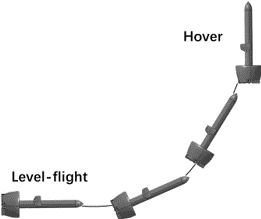
\includegraphics[height=5 cm,width=0.5\linewidth]{chapter3/CA.png}}\label{fig:CA}\\
    \hspace{-6mm}(\textbf{a}) 连续上升过渡\\
    \hspace{-6mm}{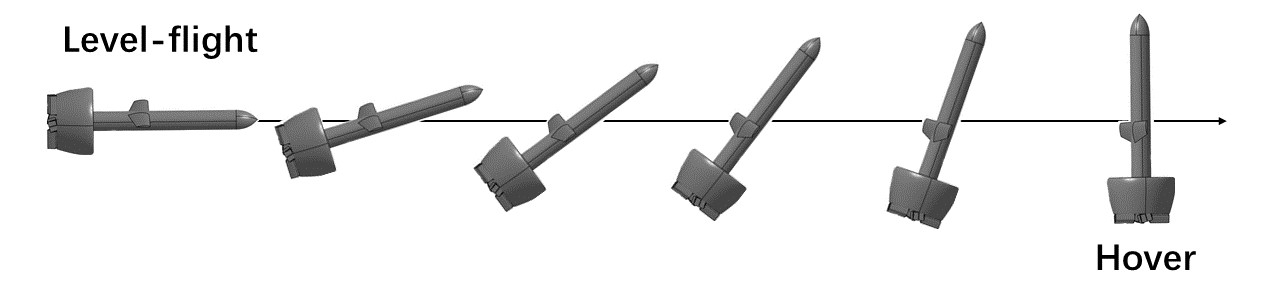
\includegraphics[width=1\linewidth]{chapter3/neat.jpg}}\label{fig:neat}\\
    \hspace{-6mm}(\textbf{b}) 定高过渡
    \end{tabular}
    \caption{常见过渡方式}
    \label{cmp} 
\end{figure}
对于具备大推重比的无人机来说,实现连续上升过渡是相对较为容易实现的,因为在该过渡过程中,无人机一直保持低攻角状态,不会发生失速现象,
这使得其动力学方程能够被线性化处理,从而简化了控制器的设计。进一步地,从能量转换的视角考虑,在连续上升过程中,无人机把动能转化为了
重力势能。相对地,在定高过渡阶段,无人机则需要利用空气阻力来降低动能。因此,与定高过渡相比,连续上升过渡通常能实现更短的过渡时间。

然而,与定高过渡相比,这种过渡方式存在两个明显的劣势:
首先,由于连续上升过渡会导致显著的高度变化,它不太适合那些对起降空间有严格限制的军事任务,此外,高度的改变还可能影响其在战场上的隐蔽性。
第二、连续上升过渡并不适合用于需要频繁起飞与降落的任务,因为与定高过渡相比,其会浪费更多的能量在垂直起飞与降落阶段,造成
工作效率的降低。

而对于定高过渡而言,其水平高度几乎不发生变化,这也意味着其攻角会经历$0^\circ \sim 90^\circ$的变化,导致失速现象的产生,同时受高度变化约束影响,
速度曲线的可行解空间也变得狭窄,控制量也容易达到饱和。文献\parencite{1022766347.nh}指出:在定高过渡,尤其是定高逆过渡过程中,仅当无人机的状态
进入某一特定解空间内时,无人机才能完成定高过渡,否则无人机会进入不可控状态导致过渡失败从而变回初始悬停状态。此外,与其他利用复合翼实现垂直起降功能
的无人机相比,涵道风扇尾座式无人机(DFTSUAV)面临更为复杂的空气动力学机制也对控制器设计带来了挑战。

因此,深入研究涵道风扇尾座式无人机(DFTSUAV)在定高逆过渡阶段的控制策略显得尤为重要。
这一研究的必要性不仅源于DFTSUAV所特有的挑战如:广泛变化的攻角引发的失速风险、高度约束下缩小的可行解空间以及复杂空气动力学对控制策略设计的挑战,
也由于其过渡性能的优化对提高任务适应性和执行效率方面的潜在工程价值。
\section{国内外研究现状}
\subsection{涵道风扇尾座式飞行器研究现状}
涵道风扇螺旋桨是一种特殊气动构型,其内部安装螺旋桨,外围则由环形涵道包裹,被广泛应用于各种飞行器的推力或升力装置中。其中,涵道不仅可以被视为环形机翼提供升力从而提供涵道风扇飞行器高速前飞能力,
而且相较于传统旋翼/直升机涵道提升了无人机的安全性、隐蔽性、气动效率。

因此自1980年起,应美国海军陆战队作战所需,美国Sandia National Lab第一次提出了涵道风扇飞行器的概念,但最终由于飞行控制技术的受限,该计划最终被迫停止。
自此之后,各个团队都开始了涵道风扇飞行器的研制,如:Allied Aerospace公司的iSTAR飞行器、法国Bertin Technologies的Hover Eye飞行器、Sikorsky
公司的Cypher系列飞行器、中国航天科工二院的“天空工厂”无人机团队等。
\begin{figure}[ht]
    \centering
    \begin{subfigure}[b]{0.32\textwidth}
      \centering
      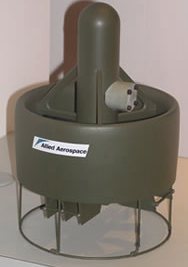
\includegraphics[height=5cm]{figure/chapter1/istar.png}
      \caption{iSTAR UAV}
      \label{fig:image1}
    \end{subfigure}
    \hfill % 这会在图片之间添加空白
    \begin{subfigure}[b]{0.32\textwidth}
      \centering
      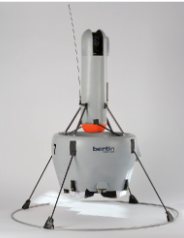
\includegraphics[height=5cm]{figure/chapter1/hovereye.png}
      \caption{Hover Eye UAV}
      \label{fig:image2}
    \end{subfigure}
    \hfill % 这会在图片之间添加空白
    \begin{subfigure}[b]{0.32\textwidth}
      \centering
      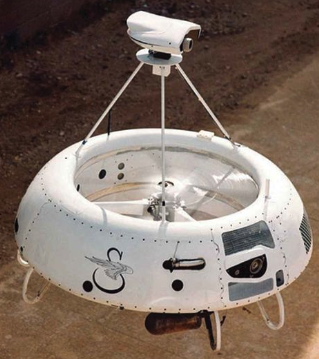
\includegraphics[height=5cm]{figure/chapter1/cypher.png}
      \caption{Cypher系列UAV}
      \label{fig:image3}
    \end{subfigure}
    \caption{各类无翼涵道飞行器}
    \label{fig:nowinguav}
\end{figure}
尽管涵道风扇飞行器具备高速巡航的优势,但其在平飞过程中依然需耗费大量能量以平衡重力,导致能源效率不佳。
因此,部分研究人员探索了将固定翼与涵道风扇飞行器结合的可能性,目的是利用机翼生成更大的升力以抵消重力,从而提升飞行器的航程和效率。

在Clandestine UAV项目的推动下,自2003年起,Aurora公司开始研发GoldenEye系列无人机,该系列以其卓越的性能受到了美国国防高级研究计划局(DARPA)的青睐,
并被纳入美国陆军未来战斗系统计划。Stephen Morris,一位曾参与该计划的重要成员,后来加入了Martin UAV(现为Shield AI),以GoldenEye为基础,负责并研发了
目前最广为人知的V-Bat涵道风扇尾座式无人机。自2008年起,V-Bat无人机经历了多次原型机的验证与调整,最终在2016年完成首次飞行测试,并在2018年成功执行了针对印度陆军在山地和丛林环境下的演示飞行。
2023年3月,V-Bat无人机正式被选为参与美国陆军未来战术无人机系统计划的一部分,目前已经成为美国陆军战队和海军演习的重点军事力量。
类似的,韩国KAIST实验室的Yeondeuk Jung等人研发了一款重量18.5kg,翼展2m,有效载荷1kg,最小连续飞行时间30分钟的涵道风扇尾座式飞行器,并重点研究了其气动建模方式和飞行模态转换控制方法。

而我国在这一机型上起步较晚,比较有代表性的是2017年华南理工大学自动化学院研发出的小型DFTSUAV,其平飞巡航速度可达20m/s,可以完成各种复杂的机动动作,
并重点研究了该类无人机的气动特性、飞行控制转换、过渡走廊、控制分配等关键技术,填补了国内这方面的空白。
\begin{figure}[ht]
    \centering
    \begin{subfigure}[b]{0.23\textwidth}
      \centering
      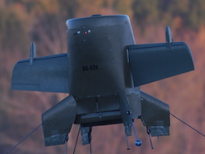
\includegraphics[height=3cm]{figure/chapter1/goldeneye.png}
      \caption{GoldenEye}
      \label{fig:image4}
    \end{subfigure}
    \hspace{6pt} % 添加5pt的水平空间
    \begin{subfigure}[b]{0.23\textwidth}
      \centering
      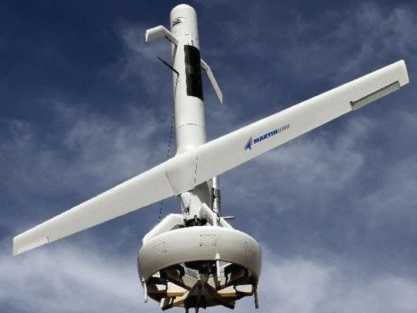
\includegraphics[height=3cm]{figure/chapter1/V-bat.png}
      \caption{V-Bat}
      \label{fig:image5}
    \end{subfigure}
    \begin{subfigure}[b]{0.23\textwidth}
      \centering
      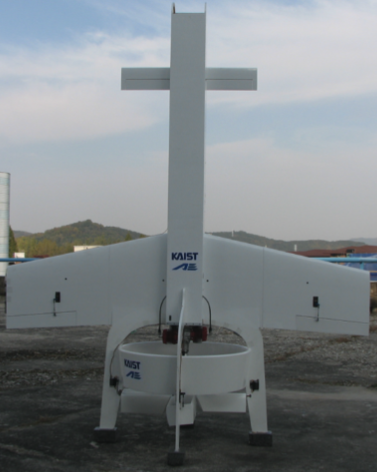
\includegraphics[height=3cm]{figure/chapter1/KAIST.png}
      \caption{KAIST DFTSUAV}
      \label{fig:image6}
    \end{subfigure}
    \begin{subfigure}[b]{0.23\textwidth}
      \centering
      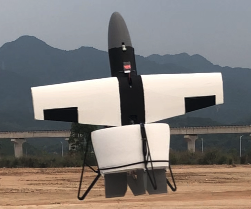
\includegraphics[height=3cm]{figure/chapter1/china.png}
      \caption{华南理工大学}
      \label{fig:image7}
    \end{subfigure}
    \caption{各类有翼涵道飞行器}
    \label{fig:winguav}
\end{figure}
\subsection{过渡过程控制研究现状}
通常来说,解决尾座式垂直起降无人机过渡控制问题一般需要先对过渡过程进行速度轨迹设计,然后再结合过渡过程控制器实施控制策略,其设计流程如\autoref{fig:controlscheme}所示。
\begin{figure}[H]
    \centering
    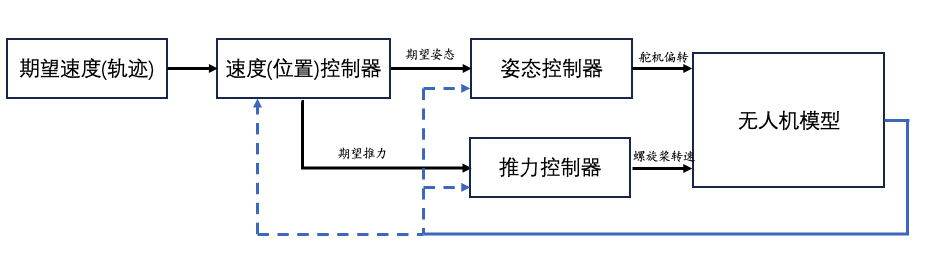
\includegraphics[width=1.0\textwidth]{figure/chapter1/控制流程.png}
    \caption{\label{fig:controlscheme}过渡模态控制}
\end{figure}

当前国内外对过渡过程控制的研究主要主要聚焦于过渡控制器设计和过渡轨迹优化两方面,其中,过渡轨迹设计方法的研究主要可分为三种:
分别是基于经验的过渡过程轨迹设计,基于过渡走廊的过渡过程轨迹设计和基于最优控制的过渡过程轨迹设计\cite{1018875946.nh}。
\begin{itemize}

    \item [1.] 基于经验的过渡轨迹设计方法\\
    \hspace*{2em}基于经验的过渡轨迹设计方法以其直观和简洁性在工程实践中得到了广泛应用。
    例如,开源飞控PX4通过施加一个恒定的推力输入和一个基于经验的线性变化俯仰角来指导飞行器完成过渡阶段\cite{meier2015px4}。
    然而,在实际应用中,PX4过渡方式可能会引起显著的飞行高度变化和执行器输出。
    Green等通过直接给定90度的俯仰角阶跃指令来实现快速连续上升过渡,但这种方法同样会导致高度的显著变化\cite{green2005mav}。
    Yeondeuk Jung等对期望攻角和航迹倾角采用分段线性函数进行设定,并利用内环的PID控制器结合外环的动态逆控制器,成功实现了了从悬停到水平飞行的正过渡控制\cite{jeong2010transition}。
    Argyle等根据简单的三角函数来规划期望的俯仰角及机体速度曲线,通过融合PID控制与前馈控制,实现了无人机的正逆过渡,但该方法的逆过渡性能表现较差,拥有几乎40m的高度损失\cite{argyle2013vertical}。
    Matthew则设计了一条简单的匀减速期望速度曲线,并提出了一种改进的总能量控制系统(Total Energy Control System, TECS),以实施控制,该方法成功地实现了在过渡期间保持无人机高度恒定的目标。
    然而,这种控制方法的平均过渡时间较长,接近10秒\cite{argyle2016modeling}。
    Alejandro和Gerardo通过确保攻角维持在最优升阻比的条件下,设计了理想的机体速度曲线,并利用RNN神经网络对飞行动力学模型进行学习,从而设计了一种基于模型的反馈线性化控制器以实现过渡控制\cite{flores2020transition}。
    
    \item [2.] 基于过渡走廊的过渡轨迹设计方法\\
    \hspace*{2em}基于过渡走廊的过渡轨迹设计方法,其核心原理在于对过渡阶段的动力学模型做出假设,确保无人机的合力及合力矩能够配平,近似达到零的状态。基于这一假设,通过所有可能的配平点建立相应的过渡走廊边界,从而在所求解的过渡走廊内,
    规划出合适的的速度曲线,以指导无人机完成过渡阶段的飞行。
    程子欢等基于定高过渡的飞行特性并结合结合无人机纵向动力学模型,在合力矩和垂向力为零的假设下,计算出无人机的‘俯仰角-速度-加速度’的过渡走廊。根据该过渡走廊的边界,设计无人机过渡过程中的期望速度曲线,
    并使用基于神经网络补偿未知干扰的自适应控制方法进行过渡过程控制\cite{cheng2022transition,cheng2020neural}。
    Naldi和Marconi依据无人机在悬停模态与水平飞行模态下的动力学特性,建立了‘攻角-飞行速度’的过渡走廊,并通过有限运动单元组合生成近似解,作为伪谱法优化的初始猜测,求解出最小能量和最短时间的垂直起降无人机最优过渡轨迹\cite{naldi2011optimal}。
    匡敏驰综合考虑了迎角、舵面偏转角、螺旋桨转速以及电机输出功率的约束,建立了‘俯仰角-飞行速度’的过渡走廊,并使用拟牛顿法求解最优过渡轨迹,最终结合线性二次调节器进行过渡过程控制\cite{1018875946.nh}。
    
    \item [3.]基于最优控制的过渡轨迹设计方法\\
    \hspace*{2em}基于最优控制的过渡轨迹设计方法通常要求无人机在过渡阶段中某些性能指标达到最优或近似最优从而视其为最优控制问题进行求解。常见的过渡性能指标包括:过渡时间最短、过渡过程高度变化最小、过渡能量最优等。
    为了分析有无襟翼时最优轨迹的差异,Kubo等使用序列二次规划算法求解了以过渡时间、过渡高度变化以及控制量变化率为性能指标的最优控制问题,证明了增升装置可以提升一定的无人机下降速率\cite{kubo2008tail}。
    Verling等以离线优化的方式通过MATALB的fmincon函数结合内点法最小化过渡时间与过渡过程高度变化,再根据离线优化的推力控制量和俯仰角进行前馈控制和姿态控制\cite{verling2017model}。
    Banazadeh和Taymourtash以推力矢量尾座式无人机为研究对象通过将优化问题转换为非线性规划问题再结合改进的梯度下降算法进行优化求解,最终得到了接近最优的无人机过渡轨迹\cite{banazadeh2016optimal}。
    Oosedo等人使用序列二次规划算法最小化过渡时间与高度损失,再根据求解出的优化轨迹结合查表法使用PID控制器进行跟踪控制\cite{oosedo2017optimal}。
    Li等人使用切比雪夫伪谱法最小化控制成本并考虑了垂向速度约束进而对垂向高度变化进行优化\cite{li2020transition}。

\end{itemize}

总的来说,上述三种做法互有优劣。基于经验的设计方法以其简便性为特点,然而,这种方法可能无法完全符合无人机的动力学特性,且难以确保过渡阶段的性能表现。
而基于过渡走廊的方法需要对无人机动力学模型的深入分析,并在状态和控制约束下建立可行的状态空间,但该方法对动力学模型的精确性有较高要求,且在实际飞行
中难以维持某些理想化约束(例如角速度变化率恒为零),导致实施策略可能过于保守,影响过渡性能。
基于最优控制的方法能够在一定程度上确保无人机过渡性能的最优化,但相比之下,这种方法的计算量较大,通常依赖于离线优化来生成轨迹,难以适应实时变化的需求。
此外,该方法未充分考虑模型失配及外部干扰的影响,可能因缺乏鲁棒性而难以在实际中使用。

\subsection{强化学习研究现状}
强化学习(Reinforcement Learning,RL),以贝尔曼最优性原理为基础,作为一种面向最优控制问题的方法论,在控制领域展现出其逐步增长的研究与应用热度,
其基于探索与利用的思想,为非线性系统的高效实时在线控制提供了一系列具有潜在应用价值的解决策略。

2023年,苏黎世大学的Elia Kaufmann等研究者在《Nature》上发表了一篇关于基于强化学习的竞速无人机控制策略的研究,该策略在多次测试中成功超越了世界冠军。
不同于过去强化学习在实践中主要应用于规划的工作,Kaufmann等采用近端策略优化(Proximal Policy Optimization, PPO)算法,将规划与控制整合,通过接收低维状态信
息输入并通过两层多层感知器(MLP)神经网络,输出推力与角速度,结合比例-积分-微分(PID)控制器进行精确控制\cite{kaufmann2023champion}。

同年,Song等在无人机竞速任务上应用相同的控制框架,展现出其在特定场景下超越最优控制方法的潜力。作者指出,传统的规划与控制分层解决方案限制了控制器的控制范围,
在面对模型未建模动态问题时,分层会导致性能下降\cite{Song_2023}。而RL可以结合领域随机化等技术更好地处理不确定性。
Robert Penicka在类似控制框架下,结合经典路径规划算法,实现了四旋翼无人机在复杂环境中的最短时间飞行,表明了RL在最优控制问题上的潜力\cite{penicka2022learning}。

然而,强化学习在最优控制领域的应用仍面临挑战。首先,关于约束的处理,主流方法通过调整奖励函数进行适配,
如\parencite{penicka2022learning}中对过大或过小的速度进行惩罚,
但在处理多重约束时易陷入奖励函数设计的困境,且在训练过程中可能违反约束条件。
其次,尽管相较于传统的最优控制方法,强化学习在处理模型不确定性方面表现出优势,但其在面对训练分布以外的测试场景时,常显示出较弱的鲁棒性和泛化能力。

针对这些挑战,约束强化学习(Constrained RL)和鲁棒强化学习(Robust RL)成为强化学习在机器人领域内的研究重点。
约束强化学习(Constrained RL)与2015年由García 和 Fernández提出,侧重于在训练或部署阶段保证智能体的安全性能,同时满足特定的性能约束。例如:
Chen等人通过将约束转化为惩罚信号并利用拉格朗日乘子法集成至奖励函数中,采用双尺度原始对偶算法进行更新以保证算法的收敛性。\cite{tessler2018reward}。
传统拉格朗日方法可能导致约束在边界处的振动,而Adam等人通过应用PID算法调整拉格朗日乘子的更新策略,有效减少了振荡现象。\cite{stooke2020responsive}。
Achiam在TRPO算算法的基础上扩展,将约束进行一阶近似,并通过Karush–Kuhn–Tucker条件进行求解,其虽然可以严格保证约束满足,但其计算代价高昂,不适合在多约束和大规模环境中使用\cite{achiam2017constrained}。
除了借助拉格朗日乘子法进行约束优化求解外,Liu等人基于PPO算法使用内点法对策略进行优化,使用对数障碍函数对约束加以惩罚,非常适合多约束环境下问题的求解,
然而,内点法要求策略的初始解必须满足约束,这也极大限制了其应用\cite{liu2020ipo}。
Aivar等人提出了一种基于状态增广的约束强化学习算法,仅通过对环境进行改动,就可以获得稳定的安全性能表现\cite{sootla2022saute}。
Dalal等人并未使用优化思想求解,而是离线的训练了一个安全层,将所有不安全的动作投影到安全区域,从而保证约束满足\cite{dalal2018safe}。

鲁棒强化学习(Roubust RL)旨在提升算法的鲁棒性,确保在最不利条件下最大化累计回报。
通常情况下,鲁棒强化学习通过对环境参数进行人为干扰,如动力学参数的质量、惯量、摩擦系数调整及传感器噪声引入等,增强算法的鲁棒性性。
因此,Jiang等提出MRPO算法,对环境参数进行均匀采样,并在轨迹中筛选中表现较差的一批,令策略朝最差环境方向进行跟新\cite{jiang2021monotonic}。
RARL采用零和博弈的思想,生成’对手‘智能体改变环境参数令回报最小化,而’我方‘智能体则需最大化对应环境下的期望回报,提升智能体的鲁棒性\cite{pinto2017robust}。
WR2L是将模型参数化,并计算模型梯度令模型朝回报最小化方向更新,并对模型变化进行沃瑟斯坦距离约束,然后在对应的模型上进行策略迭代更新。\cite{abdullah2019wasserstein}
由于鲁棒强化学习通常是对环境参数进行扰动,所以该问题也可以被视为一个部分状态可观测问题,通过引入带有记忆能力的神经网络来解决\cite{ni2021recurrent}。
例如:Alessio在研究针对强化学习策略的最优攻击手段时发现带有记忆能力的网络结构能够更好地处理干扰\cite{russo2011dynamics}。
Huan Zhang提出了一种学习对手交替训练框架,找到一个最佳‘对手’来扰动状态观测进而提升了智能体的鲁棒性,并通过实验发现基于时序神经网络结构的策略往往拥有更高的鲁棒性\cite{zhang2021robust}。

目前,应用强化学习算法于无人机过渡控制的研究较少。比较突出的是:Xu提出的一种基于强化学习算法的复合翼无人机过渡控制算法,通过引入误差积分状态量,提升了无人机
的鲁棒性和泛化性,可以适应各种不同配置的无人机\cite{xu2019learning};
Yuksek等针对推力矢量无人机设计了以强化学习为辅助回路,输出推力变化量并结合自适应动态逆的控制框架,实现了正向过渡\cite{yuksek2022transition}。
然而,值得注意的是,在这些过渡控制框架中,强化学习主要扮演底层控制器的角色,并未涉及过渡轨迹的优化问题。

需要更改综上所述,过渡
这表明,在未来的研究中,如何利用强化学习算法
同时完成过渡轨迹优化和过渡过程控制,将是探索无人机高效过渡控制策略的重要方向。
\section{研究内容与主要贡献}
随着垂直起降无人机的大力发展和对军事任务中无人机机动性能的要求,越来越多的研究人员开始关注垂直起降无人机在过渡过程中轨迹的最优性。
本文面对涵道风扇尾座式垂直起降无人机逆过渡模态转换中的飞行控制问题进行研究,针对过渡时间最短与高度变化最小两个指标,使用约束强化
学习算法展开深入研究。本文内容结构如图所示:
\begin{figure}[htbp]
    \centering
    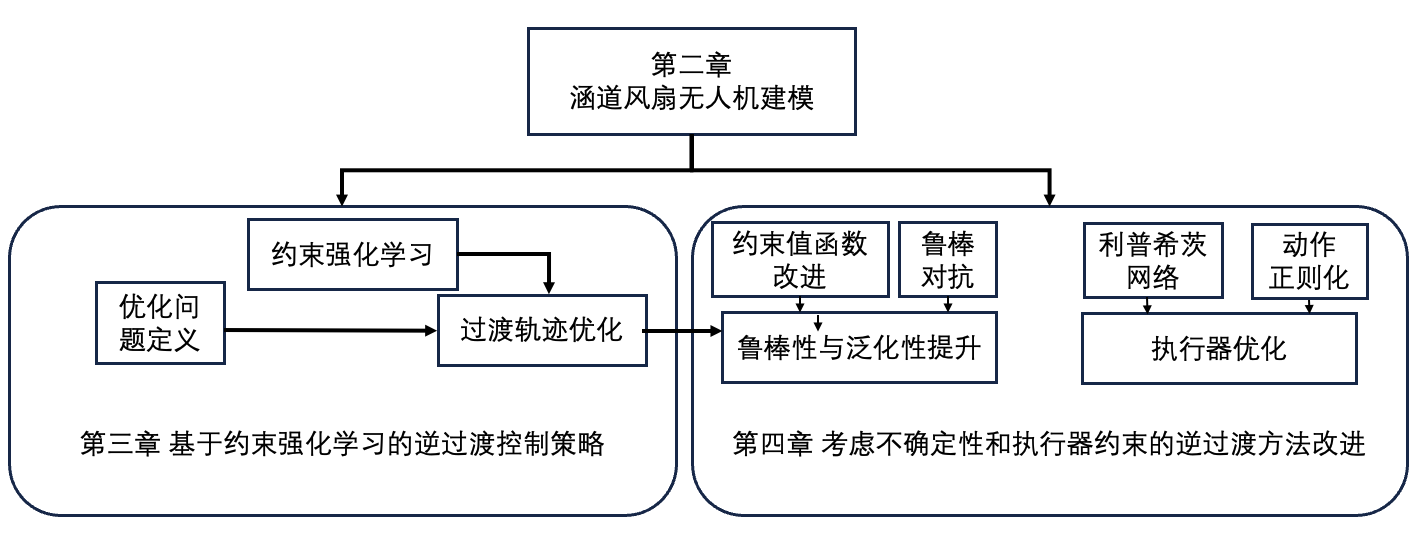
\includegraphics[width=1.0\textwidth]{figure/chapter1/主要研究内容.png}
    \caption{\label{fig:architecture}本文主要研究内容}
\end{figure}

本文主要分为五章,各章节主要内容如下:

第一章介绍了所研究的涵道风扇尾座式无人机DFTSUAV的相关背景和过渡过程轨迹优化的研究意义,并分别对过渡控制方法和强化学习算法的研究现状进行了综述,
最后介绍了本文主要研究内容与贡献。

第二章建立了涵道风扇尾座式无人机的六自由度仿真模型并介绍了强化学习的相关背景知识。首先对本文使用的坐标系及相关转换进行介绍;接着分析
无人机各个结构,描述其动力学机理,最后建立了涵道风扇尾座式无人机六自由度非线性动力学模型。

第三章建立了基于约束强化学习的逆过渡控制方案。首先,对无人机横纵向解耦,并对纵向逆过渡优化问题进行定义,介绍了快速定高过渡问题的数学形式,
然后使用约束强化学习结合课程学习对无人机控制策略进行优化;最后通过仿真实验,证明了约束强化学习算法和课程学习引入的必要性,并与总能量控制算法进行对比,说明
了强化学习算法优越性,并与基于伪谱法的最优控制算法进行了对比,说明了该方案在逆过渡轨迹优化问题上具备接近最优的能力。最终,结合横侧向控
制器,实现了无人机六自由度模型仿真,进一步说明了方法的有效性。

第四章考虑现实世界中存在的不确定性干扰,对第三章的方案进行了改进。首先,建立了真实世界中可能存在的干扰分布,并重点描述了
风干扰的数学模型,然后使用领域随机化技术结合并行框架提升无人机的鲁棒性与泛化性,同时,针对领域随机化引入的训练分布不稳定问题,
提出了价值约束拉格朗日近端策略优化算法(VCPPOLag),优化了无人机在不确定性干扰下的过渡性能。最后,通过仿真验证了所提方法的有效性
和必要性,并展示了存在干扰下无人机逆过渡控制策略的鲁棒性与泛化性能。

第五章为总结与展望,针对本文中存在的缺点与不足进行回顾并提出后续展望。

本文的主要贡献如下:

(1) 本文结合时间最短与高度变化最小两个优化指标,提出了‘快速定高过渡’的过渡方式,并将过渡轨迹优化与过渡过程控制视为一个整体,
使用约束强化学习算法进行优化,并通过仿真验证与对比实验说明了该方法的优越性,为同类型无人机提出了另外一种解决思路。

(2) 本文面对环境不确定性,提出了一种结合价值约束的约束强化学习算法,该方案通过将约束与优化问题互换,成功地避免了传统约束强化
学习算法成本阈值难以确定的问题。
\chapter{涵道风扇式无人机数学模型}
\section{引言}
本章主要对过渡过程中涵道风扇无人机数学模型以及强化学习的相关知识进行简要概述。涵道风扇式无人机在实现过渡过程中,其飞行姿态会发生
剧烈的变化,因此建立一个能够精准地描述其非线性特性的仿真数学模型是设计过渡策略的前提。

本章首先介绍了描述无人机运动所需要的坐标系
及运动参数,然后详细介绍了涵道风扇式无人机的结构,并针对涵道风扇式无人机的每个关键模块介绍其物理机理,最后基于牛顿-欧拉方法并结合
动力学与运动学方程建立涵道风扇式无人机六自由度数学模型,为后续强化学习算法设计奠定了基础。
\section{坐标系及其变换}
\subsection{常用坐标系与无人机运动参数}
\label{sec:1}
无人机的六自由度运动包括平移和旋转运动,为方便描述无人机的运动状态,引入如下坐标系:
\begin{figure}[htbp]
    \centering
    \begin{minipage}{.49\linewidth}
        \centering
        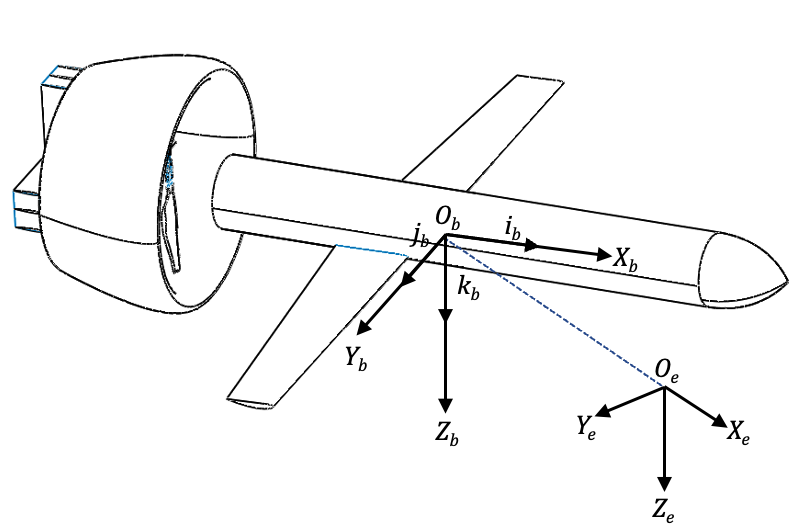
\includegraphics[width=\linewidth]{coordinate.png}
        \caption{地面坐标系及机体坐标系}
        \label{fig:coordinate}
    \end{minipage}
    \hfill
    \begin{minipage}{.49\linewidth}
        \centering
        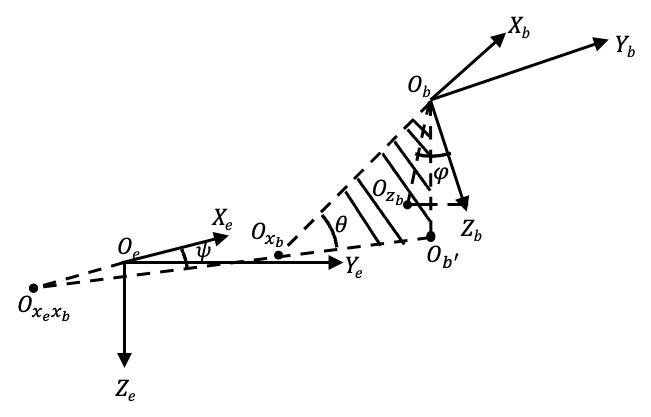
\includegraphics[width=\linewidth]{euler.png}
        \caption{欧拉角}
        \label{fig:euler}
    \end{minipage}
\end{figure}
\begin{itemize}
    \item [1.] 

        地面坐标系:地面坐标系$o_{e}x_{e}y_{e}z_{e}$定义为与地球表面固连的坐标系,通常用于研究无人机相对于地面的运动状态,确定机体的三维位置,忽略地球曲率,即将地球表面假设
        成平面。通常以无人机起飞位置作为坐标原点$o_{e}$,先让$o_{e}x_{e}$轴在水平面内指向某一方向,$o_{e}z_{e}$轴垂直与地面向下,然后以右手定则确定$o_{e}y_{e}$轴。       
    \item [2.]

        机体坐标系:机体坐标系$o_{b}x_{b}y_{b}z_{b}$与无人机机体固连。其原点$o_{b}$选取在无人机质心上;$o_{b}x_{b}$轴在无人机对称平面内沿机身轴线指向前方;
        $o_{b}z_{b}$在无人机对称平面内,垂直于$o_{b}x_{b}$轴向下,通过右手定则可确定$o_{b}y_{b}$。机体坐标系与地面坐标系的关系如\autoref{fig:coordinate}所示。
        机体坐标系相对于地面坐标系的方位,也是无人机在空中的姿态,通常可以用三个欧拉角表示,分别是俯仰角$\theta$、滚转角$\phi$、偏航角$\psi$,如\autoref{fig:euler}。

        图中$o_{b^{'}}$表示$o_{b}$在平面$o_{e}x_{e}y_{e}z_{e}$上的投影,$o_{x_{b}}$表示$x_{b}o_{b}$延长线与平面$o_{e}x_{e}y_{e}$的交点,$o_{b}o_{z_{b}}$表示
        $o_{b}z_{b}$在通过机体轴$o_{b}x_{b}$的铅锤面$o_{b}o_{x_{b}}o_{b^{'}}$上的投影;$o_{x_{e}x_{b}}$表示$x_{e}o_{e}$延长线与$o_{b^{'}}o_{x_{b}}$延长线的交点。

        其中,俯仰角$\theta$即是$o_{b}x_{b}$轴与平面$o_{e}x_{e}y_{e}z_{e}$的夹角,如果$o_{b}x_{b}$轴指向上方为正,否则为负。俯仰角实质上是描述无人机相对低面
        低头或抬头程度的物理量。
        滚转角$\phi$即是$o_{b}z_{b}$轴与铅锤面$o_{b}o_{x_{b}}o_{b^{'}}$之间的夹角,取$o_{b}z_{b}$轴指向铅锤面$o_{b}o_{x_{b}}o_{b^{'}}$的左方为正,
        否则为负。滚转角实质上是描述无人机绕其纵轴滚转程度的物理量。
        偏航角$\psi$即是$o_{b}x_{b}$轴在平面$o_{e}x_{e}y_{e}z_{e}$上的投影与$o_{e}x_{e}$延长线的夹角。取地面坐标系顺时针转动为正,否则为负。偏航角实质上是
        描述无人机偏离航线程度的物理量。
        \item [3.]
        \begin{figure}
            \centering
            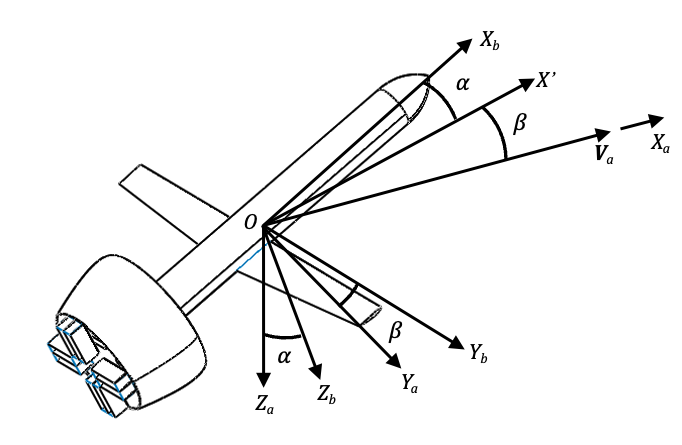
\includegraphics[width=0.5\textwidth]{stabilityframe.png}
            \caption{\label{fig:stabilityframe}气流坐标系与机体坐标系}
        \end{figure}
        气流坐标系:气流坐标系$ox_{a}y_{a}z_{a}$定义为与机体固连的坐标系。原点$o$固定在无人机的瞬时质心伤;$ox_{a}$轴与无人机速度矢量$V_{a}$重合,$oz_{a}$轴位于无人机对称平面
        内,垂直于$ox_{a}$轴指向下方;然后可以以右手定则确定$oy_{a}$轴。无人机的气动力在气流坐标系下很容易表示,因此,通常需要使用攻角$\alpha$和侧滑角$\beta$来进行气流坐标系与机
        体坐标系下的转换,如\autoref{fig:stabilityframe}所示。攻角$\alpha$定义为飞行速度矢量$V_{a}$在无人机对称平面上的投影与机体轴$ox_{b}$之间的夹角。侧滑角$\beta$定义为飞
        行速度矢量$V_{a}$与无人机对称平面之间的夹角。
\end{itemize}

\subsection{坐标变换}
在建立无人机运动方程前,还需要知道各坐标系之间的相互投影关系,即坐标转换矩阵。\\
1.地面坐标系与机体坐标系间的变换:\\

对于无人机过渡过程而言,地面坐标系与机体坐标系之间的变换需要特殊的旋转顺序才能描述,这是因为无人机的过渡过程通常要求俯仰角变化至接近$90^\circ$,
而在在传统的“$ZYX$”旋转顺序下,俯仰角在$90^\circ$时会存在奇异的情况,导致旋转矩阵计算出错。

由于过渡过程中,横侧向几乎不发生大角度变化,因此本文采用了“$ZXY$”旋转顺序定义的欧拉角,在该定义下,俯仰角的取值范围扩充至$\left [ -180^\circ,180^\circ \right ]$,
奇异点变成了$90^\circ$滚转角。

对于“$ZXY$”旋转顺序,每次旋转的角度依次为:$\psi$(偏航角)、$\phi$(滚转角)、$\theta$(俯仰角),绕各种转动的坐标
转换矩阵分别如下:
\begin{align}
    R_{z}(\psi) & = \begin{bmatrix}
    \cos\psi&  -\sin\psi& 0\\
    \sin\psi&  \cos\psi& 0\\
    0&  0& 1
    \end{bmatrix}\\
    R_{x}(\phi) & = \begin{bmatrix}
    1&  0& 0\\
    0&  \cos\phi& -\sin\phi\\
    0&  \sin\phi& \cos\phi
    \end{bmatrix}\\
    R_{y}(\theta) & = \begin{bmatrix}
    \cos\theta&  0& \sin\theta\\
    0&  1& 0\\
    -\sin\theta&  0& \cos\theta
    \end{bmatrix}
\end{align}
由此可得"$ZXY$"旋转顺序下由机体坐标系到地面坐标系的旋转矩阵$R_{b}^{e}$:
\begin{align}
    R_{b}^{e} &= R_{z}(\psi)R_{x}(\phi)R_{y}(\theta) \nonumber \\
    &= \begin{bmatrix}
    \cos \theta\cos \psi -\sin \phi \sin \theta \sin \psi&  -\sin\psi\cos\phi& \cos\psi\sin\theta+\sin\psi\sin\phi\cos\theta  \\
    \sin\psi\cos\theta+\cos\psi\sin\phi\sin\theta&  \cos\psi\cos\phi& \sin\psi\sin\theta-\cos\psi\sin\phi\cos\theta\\
    -\cos\phi\sin\theta&  \sin\phi& \cos\phi\cos\theta
    \end{bmatrix}
\end{align}
2. 气流坐标系与机体坐标系间的变换:\\

由气流坐标系定义可知,机体坐标系与气流坐标系之间的关系可以只用攻角和侧滑角来描述,对应旋转矩阵如下:
\begin{align}
    L(\alpha)&=
    \begin{bmatrix}
    \cos\alpha&  0& -\sin\alpha\\
    0&  1& 0\\
    \sin\alpha &  0& \cos\alpha 
    \end{bmatrix} \\
    L(\beta)&=
    \begin{bmatrix}
    \cos\beta&  \sin\beta& 0\\
    -\sin\beta&  \cos\beta& 0\\
    0 &  0& 1 
    \end{bmatrix}
\end{align}

由此可得气流坐标系到机体坐标系的转换矩阵为:
\begin{align}
    L_{a}^{b}&= L(\alpha)L(\beta) \nonumber \\
    &=
    \begin{bmatrix}
    \cos\alpha\cos\beta&  \cos\alpha\sin\beta& -\sin\alpha\\
    -\sin\beta&  \cos\beta& 0\\
    \sin\alpha\cos\beta &  \sin\alpha\sin\beta& \cos\alpha 
    \end{bmatrix} 
    \label{eq:Lab}
\end{align}
% \end{itemize}                                         
\section{涵道风扇尾座式垂直起降无人机运动学模型}
运动学与质量与受力无关,只研究无人机位置、速度、姿态和角速度等变量。通常情况下,运动学模型的输入为速度和角速度,输出为位置和姿态。
在刚体假设下,无人机六自由度运动学方程可以由质点的运动学方程和欧拉运动学方程描述,分别为:
\begin{equation}
    \left\{\begin{array}{l}
        {\dot{\mathbf{p}}}^{e}={\mathbf{v}}^{e} \\
        \dot{\mathbf{\Theta}}=\mathbf{Q} {\mathbf{\omega}}^{b} \\
        \end{array}\right.
\end{equation}
其中,$\mathbf{p}$表示为无人机的位置向量,$\mathbf{v}^{b}$表示无人机在机体坐标系下的速度,$\mathbf{\Theta}$为无人机的欧拉角,${\mathbf{\omega}}^{b}$表示无人机的角速度,
在$ZXY$旋转顺序下
描述欧拉角变化率与角速度关系的$\mathbf{Q}$如下定义:
\begin{equation}
    \mathbf{Q} \triangleq\left[\begin{array}{ccc}
        \cos\theta & 0 & \sin\theta \\
        \sin\theta\tan\varphi  & 1 & -\cos\theta\tan\varphi  \\
        -\sin\theta/\cos\varphi  & 0 & \cos\theta/ \cos\varphi
        \end{array}\right]
\end{equation}
\section{涵道风扇尾座式垂直起降无人机动力学模型}
动力学既涉及运动又涉及无人机受力情况,与无人机的质量与转动惯量有关,动力学模型的输入为合外力与合外力矩
,输出为速度与角速度。无人机动力学模型与运动学模型一起构成了无人机飞行控制刚体六自由度模型。
\begin{figure}[htbp]
    \centering
    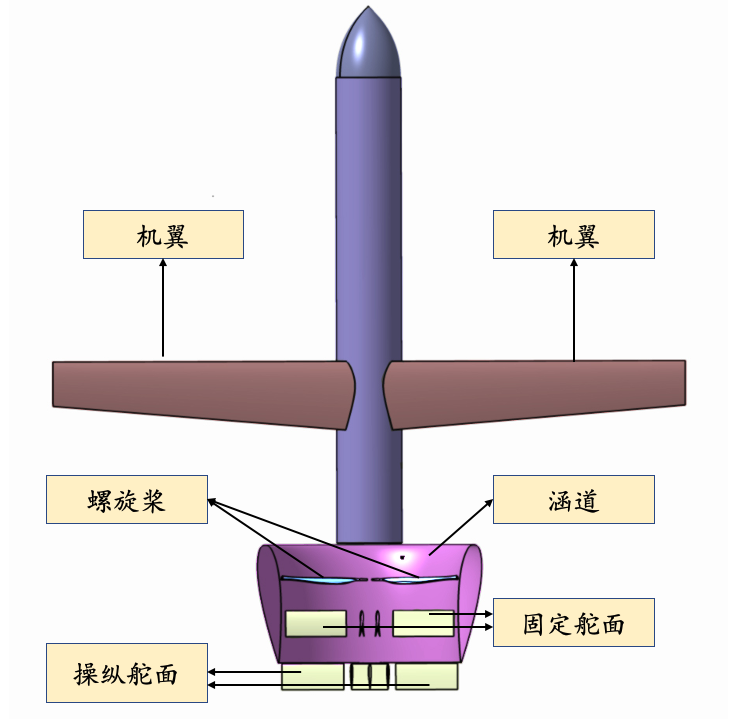
\includegraphics[width=0.4\textwidth]{wholebody.png}
    \caption{\label{fig:layout}涵道风扇式无人机总体结构图}
\end{figure}

涵道风扇式无人机可以认为主要由五个不同的子模块构成,如\autoref{fig:layout}所示,分别是:
一、涵道螺旋桨:涵道螺旋桨主要负责为无人机提供推力,是无人机悬停状态下的动力来源,其产生的诱导速度同时也会影响到舵面的操纵效率;
二、涵道:涵道为环形机翼结构,因此涵道机身本身上也会产生一定的气动力,同时由于涵道对于气流的对齐作用,涵道还会受侧风影响产生一
定的动量阻力与动量阻力矩,此外还可以减少气流损失,提高螺旋桨的气动效率;
三、操纵舵面:涵道无人机的涵道内部有四组独立偏转的操纵舵面,每组操纵舵面由三片带有翼型的矩形舵板组成,涵道下洗气流流经操纵舵面产生气动
力和气动力矩,因此通过操纵四组舵面的偏转就可以改变无人机的运动状态;
四、机翼及机身:机翼与机身会产生气动力及其产生的力矩,这也是无人机水平飞行状态下的动力来源;
五、固定舵面:固定舵面主要用来平衡悬停状态下螺旋桨产生的反扭距,提高悬停效率。
因此,定义合力$\mathbf{F}$和合力矩$\mathbf{M}$如下:
\begin{align}
    \mathbf{F} & =\mathbf{F}_{prop}+\mathbf{F}_{aero}+\mathbf{F}_{cs}+\mathbf{F}_{d}\\
    \mathbf{M} & =\mathbf{M}_{aero}+\mathbf{M}_{prop}+\mathbf{M}_{gyro}+\mathbf{M}_{cs}+\mathbf{M}_{d}+\mathbf{M}_{f}
\end{align}
其中,$\mathbf{F}_{prop}$和$\mathbf{M}_{prop}$表示涵道内部螺旋桨产生的推力与反扭力矩,
$\mathbf{F}_{aero}$和$\mathbf{M}_{aero}$表示机翼与机身上所产生的气动力和气动力矩,
$\mathbf{F}_{cs}$和$\mathbf{M}_{cs}$表示涵道底部的操纵舵面舵产生的力和力矩,
$\mathbf{F}_{d}$和$\mathbf{M}_{d}$表示涵道机身上所受到的力和力矩,
$\mathbf{M}_{f}$表示固定舵面产生的力矩,$\mathbf{M}_{gyro}$表示无人机的陀螺力矩。

综上,结合运动学和动力学模型,可得无人机六自由度运动方程为:
\begin{align}
\left\{\begin{array}{l}
    \dot{\mathbf{p}}^{e}=\mathbf{v}^{e} \\
    \dot{\mathbf{v}}^{e}=\mathbf{R}_{\mathrm{b}}^{e} \mathbf{F}+g\mathbf{e}_{3} \\
    \dot{\mathbf{\Theta}}=\mathbf{Q} {\mathbf{\omega}}^{b} \\
    \dot{\mathbf{\omega}}^{b}=\mathbf{M}+\mathbf{J}^{-1}\left(\mathbf{J} {\mathbf{\omega}}^{b} \times {\mathbf{\omega}}^{b}\right)
    \end{array}\right.
\end{align}
其中,$g$表示重力加速度,$\mathbf{e}_{3}$为地面坐标系下$Z_{e}$轴的单位向量,$\mathbf{J}$表示转动惯量矩阵,接下来会给出
相应模块的机理及具体表达式。
\subsection{涵道螺旋桨动力学}
涵道风扇式无人机的螺旋桨动力学模型极为复杂。在模拟其产生的推力时,有多种理论和方法可供选择。大多数方法在计算过程中都假设了诱导速度是已知的,
或对流场中的空速和螺旋桨的相对方向施加了严格的约束条件。

而本文使用了一种结合了基本动量理论和叶素理论的模型,最初是为具有较大展弦比的直升机旋翼设
计的,现已成功应用于涵道风扇式无人机的螺旋桨模拟。尽管在构建此模型时没有考虑涵道中的不稳定流动,该模型仍能为涵道
风扇中的螺旋桨提供相当精确的模拟效果\cite{johnson2006modeling}。其中,螺旋桨的推力和气流速度受到沿机体轴$X_{b}$的气流方向、螺旋桨的角速度以及
螺旋桨叶片的几何形状的影响,公式如下\cite{choi2012static}:
\begin{align}
    v_{b} &= \left ( u-u_{wind} \right )  + \frac{2}{3}\omega_{p}r_{p}\left ( \frac{3}{4}K_{twist}\right )\\
    T &= \frac{1+k_{aug}}{4} \left ( v_{b}-v_{i}  \right )\omega _{p}r_{p}^{2}\rho _{\infty}a_{0}bc_{p}   
\end{align}
式中,$v_{b}$表示通过螺旋桨的气流速度,$T$表示螺旋桨产生的推力,$v_{i}$表示诱导速度, $\omega_{p}$表示螺旋桨的旋转角速度, $r_{p}$表示螺旋桨的
半径,$k_{twist}$表示叶片的扭转系数,$a_{0}$表示螺旋桨旋翼叶片升力曲线斜率,$b$表示叶片个数, $c_{p}$表示螺旋桨叶片弦长, $\rho _{\infty}$
表示空气密度, $\mathbf{v}^{b}=\left [ u,v,w \right ]^{T}$表示无人机体轴下的速度,$\mathbf{v}_{wind}=\left [ u_{wind},v_{wind},w_{wind} \right ]^{T}$
表示沿机体轴的风速。

此外,涵道还会提升螺旋桨一定的气动效率\cite{myers2009aerodynamic}。涵道对于螺旋桨所产生的影响可以用$K_{aug}$来表示,
这是一个可以描述涵道对于螺旋桨的增升作用\cite{杜思亮2016轴流状态下涵道螺旋桨增升方法的数值模拟}的比例系数,$0<= k_{aug}<= 1$,当它为1时,
表示理想状态下涵道的存在可以令螺旋桨多产生一倍的推力,当它为0时,可以被认为此时不存在涵道,推力的产生只取决于螺旋桨本身。

涵道在涵道末端远场速度$v_{f}$和诱导速度$v_{i}$可以被表示为
\begin{align}
    v_{f}&=\sqrt{\left ( u-u_{wind}+v_{i}  \right )^{2}+\left (  w - w_{wind}\right ) ^{2}+\left ( v - v_{wind}\right )^{2}} \\
    v_{i}&=\frac{T}{2\rho _{\infty}\pi r_{p}^2v_{f}} 
\end{align}
然而,上述公式并不存在一个闭式解析解。因此针对这个非线性耦合代数方程组(2-13)-(2-16),采取牛顿-拉夫逊算法进行迭代求解,函数方程如下:
\begin{align}
    f\left(v_{i}\right)=v_{i}-\frac{\frac{1+k_{aug}}{4} \left(v_{b}-v_{i}\right) \omega _{p}r_{p}^{2}\rho _{\infty}a_{0}bc_{p}}{2 \rho _{\infty} \pi\left(\sqrt{\left ( u-u_{wind}+v_{i}  \right )^{2}+\left (  w - w_{wind}\right ) ^{2}+\left ( v - v_{wind}\right )^{2}}\right.}
\end{align}
在提供足够合理的初值下,通过牛顿-拉夫逊算法迭代求取函数方程零点即可对螺旋桨推力以及诱导速度进行求解。螺旋桨产生的推力如下:
\begin{align}
    \mathbf{F}_{\text {prop}}=\left[\begin{array}{c}
        T \\
        0 \\
        0
        \end{array}\right]
\end{align}

作用在旋翼上的电机功率可由下方公式计算得出\cite{任小璐2014涵道式无人飞行器建模与控制方法研究}:
\begin{align}
    P_{ind}=\frac{v_{i} T}{1+k_{aug}}
\end{align}

空气作用在旋翼上而产生的反扭力矩可表示为:
\begin{align}
    \mathbf{M}_{\text {prop}}=\left[\begin{array}{lll}
        \frac{P_{ind}}{\omega_{p}} & 0 & 0
        \end{array}\right]^{T}
\end{align}

\subsection{涵道空气动力学}
\begin{figure}[htbp]
    \centering
    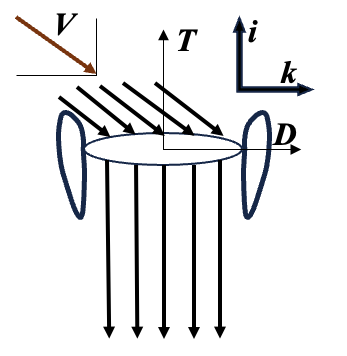
\includegraphics[width=.3\linewidth]{momentum.png}
    \caption{\label{fig:momentum}动量阻力示意图}
\end{figure}
涵道一般会被视为是无人机升力体的一部分,并不需要单独建模其作为环形机翼而产生的气动力\cite{zhang2013new}。
因此,我们将只考虑由于侧风影响产生的涵道动量阻力与动量阻力矩。

动量阻力与动量阻力矩的产生机理如下:

当来流以$V$的幅值到达涵道唇缘带动气流进入涵道时,涵道管壁将矫正来流使气流与涵道对齐,这样会在涵道上产生相应的反作用力,这种由于
侧风影响而产生的力称为动量阻力;侧风会在涵道唇口附近产生一个负压区,将涵道周围的空气吸入涵道,使唇口附近产生更大的升力,进而产生一个使无人机偏离侧风的动量阻力矩。
动量阻力与动量阻力矩的公式如下\cite{argyle2013vertical}:
\begin{align}
    \mathbf{F}_{\text {d}} & = -v_{i} \rho_{\infty} \pi r_{d}^{2}\left[\begin{array}{lll}
    0 & v & w
    \end{array}\right]^{T}\\
    \mathbf{M}_{\text {d}} & = C_{d u c t} \rho_{\infty} r_{d}\left[\begin{array}{lll}
    0 & -w|w| & v|v|
    \end{array}\right]^{T}
\end{align}
其中,$r_{d}$是涵道半径,$C_{duct}$是涵道力矩系数。
\begin{figure}[htbp]
    \centering
    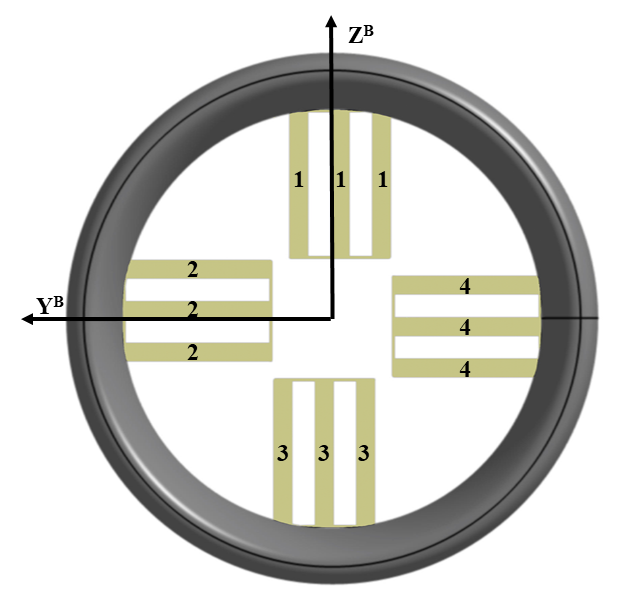
\includegraphics[width=0.3\textwidth]{vanes.png}
    \caption{\label{fig:control_vanes}操纵舵面示意图}
\end{figure}
\subsection{操纵舵面动力学}
操作舵面由四组相互独立的舵面及相应平行的导流板组成,其中1,3号舵面产生偏航力矩,2,4号舵面产生
俯仰力矩,所有舵面共同产生滚转力矩,如\autoref{fig:control_vanes}所示。本文中用$\delta_{1}$, $\delta_{2}$, $\delta_{3}$, $\delta_{4}$来
表示对应舵面组的偏转角度,最大偏转角度为30度。
由于控制舵面暴露在螺旋浆所产生的下洗流中。因此,由于每个导流板可以视为一片机翼,因此,其表面动压可以被建模为:
\begin{align}
    q_{cs}=\frac{1}{2} \rho_{\infty}\left(u-u_{wind}+v_{i}\right)^{2}
\end{align}

当使用四组操纵舵面去控制无人机的姿态运动时,控制量是冗余的。
因此本章采取了一种简单直接的控制分配方式\cite{zhang2013new}, 考虑下面的约束:
\begin{align}
    \delta_{1} = -\delta_{3}
\end{align}

控制分配形式如下:
\begin{align}
    \left[\begin{array}{l}
    \delta_{1} \\
    \delta_{2} \\
    \delta_{3} \\
    \delta_{4}
    \end{array}\right] & = \left[\begin{array}{ccc}
    0 & 0 & 0.5 \\
    0.5 & 0.5 & 0 \\
    0 & 0 & -0.5 \\
    0.5 & -0.5 & 0
    \end{array}\right]\left[\begin{array}{l}
    \delta_{x} \\
    \delta_{y} \\
    \delta_{z}
    \end{array}\right]
\end{align}
也就是说,控制系统将会根据姿态的误差输出相应的虚拟控制舵面$\delta_{x}$、$\delta_{y}$和$\delta_{z}$,
再经过控制分配得到实际的操纵舵面偏转量。因此,由于控制分配并非论文的重点,本文中后续使用的舵面偏转量实际上
是虚拟控制舵面所对应的偏转角度。
由操纵面产生的作用于机体的力和力矩可分别表示为:
\begin{align}
    \mathbf{F}_{\mathrm{cs}} & = q_{\mathrm{cs}} S_{\mathrm{v}} C_{\mathrm{L,v}}\left[\begin{array}{c}
    0\\
    -\delta_{z}  \\
    \delta_{y} 
    \end{array}\right] \\
    \mathbf{M}_{\mathrm{cs}} & = q_{\mathrm{cs}} S_{\mathrm{cs}} C_{\mathrm{L,v}}\left[\begin{array}{ccc}
    l_{1} & 0 & 0 \\
    0 & l_{2} & 0 \\
    0 & 0 & l_{2}
    \end{array}\right]\left[\begin{array}{c}
    \delta_{x} \\
    \delta_{y} \\
    \delta_{z}
    \end{array}\right]
\end{align}
其中,$C_{L,v}$表示舵面所对应的翼型的升力曲线斜率,$S_{v}$表示舵面的面积,$l_{1}$是相对于滚转轴的力臂,
$l_{2}$表示相对于俯仰/偏航轴的力臂。

\subsection{机体动力学}
在计算无人机气动力学时,我们将重点考虑机翼所受气动力,并忽略机身所受气动力\cite{zhang2013new}。
为了更好的描述无人机气动特性,给出空速、攻角和侧滑角相应计算公式如下:
\begin{align}
    V_{a} & =\sqrt{u_{r}^{2}+v_{r}^{2}+w_{r}^{2}} \\
    \alpha & =\tan ^{-1}\left(\frac{w_{r}}{u_{r}}\right) \\
    \beta & =\sin ^{-1}\left(\frac{v_{r}}{V_{a}}\right),
\end{align}
其中,
\begin{align*}
    \left\{\begin{matrix}
        u_{r} = u-u_{\text {wind }}\\
        v_{r} = v-v_{\text {wind }}\\
        w_{r} = w-w_{\text {wind }}
        \end{matrix}\right.
\end{align*}
由于垂直起降无人机在过渡过程中主要发生在纵向平面,即$o_{b}x_{b}z_{b}$平面。因此下面分别分析无人机的纵向空气动力学与横向空气动力学,并进行建模:
\subsubsection{纵向空气动力学}
无人机纵向空气动力和力矩会导致机身$i_{b}-k_{b}$平面(又称为俯仰平面)上的运动,如\autoref{fig:longitudinal}所示。图中描述了升力、阻力
和俯仰力矩,
\begin{figure}[htbp]
    \centering
    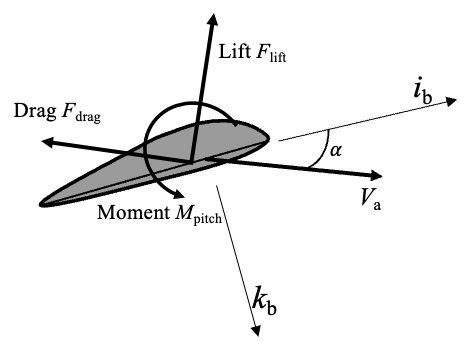
\includegraphics[width=0.5\textwidth]{airfoil.png}
    \caption{\label{fig:longitudinal}无人机纵向受空气动力分析}
\end{figure}
根据定义,升力、阻力以及俯仰力矩的变化很大程度上取决于空速与攻角,而在部分文献中,为了简化模型,通常会基于低攻角假设,对升力、阻力以及俯仰
力矩进行一阶泰勒展开,这是因为,在典型的低攻角飞行条件下,流场在飞机机身上方为层流且附着在表面,空气将以有序的方式流过飞机表面,并不会发生分
离或湍流,这种流场通常被称为准稳态流场,这种流动的稳定性和可预测性意味着气动力和力矩相对于攻角的变化是平滑的,可以使用一阶泰勒近似。

因此在低攻角工作区域范围内,气动力和力矩可以采取线性模型进行建模\cite{kikumoto2022back},公式如下:
\begin{align}
    C_{L,n}(\alpha) &= C_{L_{0}}+C_{L_{\alpha}} \alpha \\
    C_{D,n}(\alpha) &=C_{D_{0}}+C_{D_{\alpha_{1}}} \alpha+C_{D_{\alpha_{2}}} \alpha^{2} \\
    C_{m,n}(\alpha) &= C_{m_{0}}+C_{m_{\alpha}} \alpha
\end{align}
其中,下标$n$表示此时处于低攻角工作区域,下标$L$表示对应的是升力系数,下标$D$表示对应的是阻力系数,下标$m$表示对应的是俯仰力矩系数。

由于垂直起降无人机在从垂直模态转换至水平模态的过程中常常进入高攻角工作区域\cite{argyle2016modeling},而当攻角增至导致气流与机翼分离时,
升力可能会突然显著下降产生失速现象。这是因为在低攻角或中等攻角条件下,机翼上方的气流为
层流,并在流过机翼时附着在机翼上。而当攻角超过临界失速角时,气流开始从机翼顶面分离,造成湍流,机翼产生的升力因此骤减。所以在大攻角条件下,之前
的气动模型线性假设不再成立。

而当飞机由于高攻角而产生失速现象时,机翼的作用可以被近似为一块平板\cite{stengel2005flight}。基于平板理论
\cite{kikumoto2022back,stengel2005flight,puopolo2013comparison,beard2012small},当攻角大于临界失速角时,气动模型可被如下表示:
\begin{align}
    C_{L,s}(\alpha) & =2 \operatorname{sign}(\alpha) \sin ^{2}(\alpha) \cos (\alpha) \\
    C_{D,s}(\alpha) & =2 \sin ^{2}(\alpha) \\
    C_{M,s}(\alpha) & =-\operatorname{sign}(\alpha) \sin (\alpha) \sin (\alpha / 2)
\end{align}
其中,下标$s$表示此时工作在高攻角区域。

为了更好地描述上述两种气动特性,本文使用了一种基于混合函数的气动模型
,其可以适用于在较大攻角范围内($\alpha\in \left [ -180^\circ, 180^\circ\right ] $),并且可以很好的描述低攻角下的线性阶段和高攻角的失速现象,
同时为了考虑角速率对气动系数的影响,气动模型也进行了一定的修正,公式如下\cite{kikumoto2022back,beard2012small}:
\begin{align}
    C_{*} & = (1-\sigma(\alpha))C_{*,n}(\alpha)+\sigma(\alpha)C_{*,s}(\alpha) + C_{*_{q}}\frac{c}{2V_{a}}q
    \label{eq:aero}
\end{align}
其中,$*$表示下标可以是$L$,$D$和$m$,混合函数定义如下:
\begin{align}
    \sigma(\alpha) & = \frac{1+e^{-M\left(\alpha-\alpha_{s}\right)}+e^{M\left(\alpha+\alpha_{s}\right)}}{\left(1+e^{-M\left(\alpha-\alpha_{s}\right)}\right)\left(1+e^{M\left(\alpha+\alpha_{s}\right)}\right)}
\end{align}

根据计算流体力学软件,我们获得了$\left [-80^\circ, 80^\circ\right]$下气动系数与攻角的离散数据,因此我们将基于上述公式,使用Scipy中的非线性最小二乘法进行拟合,拟合曲线如\autoref{fig:aerodata}所示:
\begin{figure}[htbp]
    \centering
    \includegraphics[width=0.8\textwidth]{aerodata.png}
    \caption{\label{fig:aerodata}气动系数拟合效果示意图}
\end{figure}

可以看出,混合函数模型可以比较精准的描述气动系数随攻角变化的关系,但仍有一些误差。因此在设计控制器时,我们会考虑一定的模型气动系数失配,进行补偿。

由拟合曲线参数,可以得到$\left [-180^\circ, 180^\circ \right ]$ 范围下的气动系数与攻角关系图。纵向气动系数随攻角变化的具体关系,如\autoref{fig:aerocoeff}所示。
\begin{figure}[htbp]
    \centering
    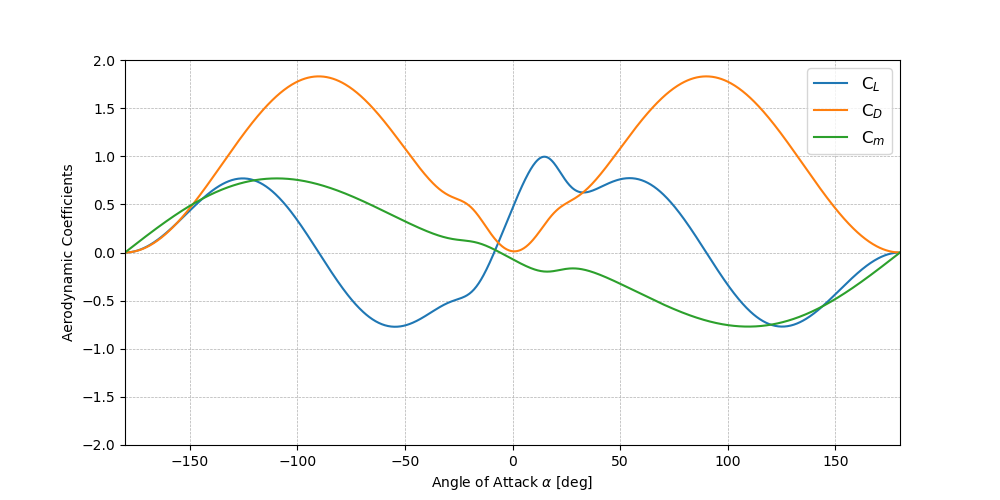
\includegraphics[width=0.8\textwidth]{aerocoeff.png}
    \caption{\label{fig:aerocoeff}无人机纵向受空气动力分析}
\end{figure}

由空气动力学可知,空气动力学的一般公式可以表示为:
\begin{align}
    L & =\frac{1}{2} \rho_{\infty} V_{a}^{2} S C_{L} \\
    D & =\frac{1}{2} \rho_{\infty} V_{a}^{2} S C_{D} \\
    m & =\frac{1}{2} \rho_{\infty} V_{a}^{2} S c C_{m}
\end{align}
其中,$C_{L},C_{D},C_{m}$由\autoref{eq:aero}计算,$L$表示升力, $D$表示阻力, $m$表示俯仰力矩,$S$表示机翼相对参考面积,c表示无人机的俯仰力臂.
\subsubsection{横向空气动力学}
无人机横向空气动力学包括由侧向力$Y$导致飞行器沿$j_{b}$轴的侧向平移运动以及受侧向力矩$l$和$n$影响的滚转和偏航运动。无人机横向空气动力学主要由
侧滑角$\beta$决定,同时还受滚转角速率$p$和偏航角速率$r$影响, 公式如下:
\begin{align}
    Y & = \frac{1}{2} \rho V_{a}^{2} S C_{Y}\left(\beta, p, r\right) \\
    l & = \frac{1}{2} \rho V_{a}^{2} S b C_{l}\left(\beta, p, r\right) \\
    n & = \frac{1}{2} \rho V_{a}^{2} S b C_{n}\left(\beta, p, r\right)
\end{align}

由于垂直起降无人机在过渡过程中横向运动的主要任务是保证稳定性,因此侧滑角的变化范围较小,可以基于一阶泰勒近似使用线性模型去描述其侧向空气动力学模型,公式如下:
\begin{align}
    C_{Y} & = C_{Y_{0}}+C_{Y_{\beta}} \beta+C_{Y_{p}} \frac{b}{2 V_{a}} p+C_{Y_{r}} \frac{b}{2 V_{a}}r\\
    C_{l} & = C_{l_{0}}+C_{l_{\beta}} \beta+C_{l_{p}} \frac{b}{2 V_{a}} p+C_{l_{r}} \frac{b}{2 V_{a}} r\\
    C_{n} & = C_{n_{0}}+C_{n_{\beta}} \beta+C_{n_{p}} \frac{b}{2 V_{a}} p+C_{n_{r}} \frac{b}{2 V_{a}} r
\end{align}

由于气动力$L,D,Y$定义在气流坐标系,因此需要结合\autoref{eq:Lab}进行坐标转换:
\begin{align}
    \mathbf{F}_{\text {aero}} & = L_{a}^{b}(\alpha ,\beta)\begin{bmatrix}
    -D\\
    -Y\\
-L
\end{bmatrix}\\
\mathbf{M}_{\text {aero}} & = \begin{bmatrix}
    l\\
    m\\
n
\end{bmatrix}
    \end{align}
\subsection{固定气动面动力学和陀螺力矩}
涵道无人机内部的固定气动面一般被设计用来平衡悬停状态下旋翼下的反扭力距。因此固定气动面对涵道轴的力矩可近似为:
\begin{align}
    \mathbf{M}_{f} & = \left[\begin{array}{lll}
    k_{f} (v_{i}+u_{r})^{2} & 0 & 0 
    \end{array}\right]^{T}
\end{align}
其中,$k_{f}$是固定舵面力矩系数。
通常情况下,陀螺力矩可以忽略不计,但当无人机执行诸如过渡等大角度机动时,陀螺力矩则不可忽略。陀螺力矩公示如下:
\begin{align}
    \mathbf{M}_{\text {gyro }} & = n_{p} \omega_{p} J_{p}\left[\begin{array}{c}
    0 \\
    -r \\
    p
    \end{array}\right]
\end{align}
其中,$n_{p}$为转子个数,$J_{p}$为螺旋桨转动惯量,$p$和$r$是滚转和偏航角速率。

\section{本章小结}
本章建立了涵道风扇式无人机的数学模型并介绍了强化学习相关的基础知识。首先定义了描述无人机运动的坐标系及其转换,给出了其运动学方程和动力学方程,
通过对涵道风扇式无人机模块化,分别对无人机动力学方程中涉及的气动力和气动力矩进行分析,并给出了其完善的无人机六自由度数学模型,为后续的过渡控制策略设计奠定了基础。
\chapter{基于强化学习的无人机逆过渡问题研究}
\section{引言}
在本章节中,我们将深入无人机动力学模型,通过横向和纵向的解耦来分别构建强化学习环境。我们的重点将放在纵向的三自由度涵道无人机动力学模型上,从优化的视角出发,阐述纵向逆过渡过程中所期望的性
能指标和约束条件。接着,我们使用结合拉格朗日乘子的近端策略优化算法实现了快速定高过渡。此外,我们还将与总能量控制算法、
最优控制和传统强化学习算法进行较,以验证所提出方法的有效性。最终,我们同样使用强化学习算法训练无人机横侧向控制器,并在六自由度动力学模型上进行仿真,进一步证明其实用性。
\section{无人机逆过渡问题描述}
在无人机过渡控制策略的设计过程中,动力学的横纵向解耦显得尤为关键。这主要基于以下考虑:
一、在涵道无人机的过渡阶段,主要的动态变化集中于纵向平面,其中空气动力的变化尤为显著,从而对纵向控制策略提出了更高的要求。相比之下,横向动力学比较简单,通常可以采用线性化处理来进行简化。
适当的模型简化假设允许我们专注于纵向的控制策略,以便构建和评估过渡策略。
二、对于强化学习训练而言,三自由度无人机模型相比于六自由度模型只有近乎一半的状态空间和动作空间,可以加快评估不同的奖励函数以及超参数设置的过程。
因此,基于无人机过渡变化主要发生纵向的假设,可以得到简化后的三自由度动力学方程与快速定高过渡问题的数学形式:
\begin{equation}
    \left\{
    \begin{aligned}
    \dot{u}&= g\sin \theta +\left (  D\cos \alpha -T-L\sin\alpha\right )/m -qw \\
    \dot{w}&= \left ( F_{d}+L\cos\alpha+D\sin\alpha +F_{cs} \right )/m+qu-g\cos\theta\\
    \dot{x}&= w\cos \theta-u\sin \theta \\
    \dot{z}&= u\cos \theta+w\sin \theta \\
    \dot{\theta}&=q\\
    \dot{q}&=\left ( m_{pitch} + M_{d} + M_{cs} \right ) /J_{y}
    \label{eq:three_dof}
    \end{aligned}
    \right.
\end{equation}
其中,无人机纵向状态量可以表示为:$X=\left [ u,w,\theta,q \right ]^{T}$, 控制量为:$U=[\omega _{p},\delta_{y}]$。
因此对于\autoref{eq:three_dof}这样的动力学方程,
期望最小化过渡时间:
\begin{align}
    J & = t_{f}
\end{align}
其中,$t_{f}$表示为终端时间,并考虑如下控制量约束和角速度约束:
\begin{align}
    \left\{\begin{matrix}
        \left | \delta _{y} \right |<30^{\circ}\\
        \omega _{pmin}<\omega _{p}<\omega _{pmax}\\
        \left | q \right |<90^{\circ}
    \end{matrix}\right.
\end{align}

角速度约束主要是为了避免因角速度过大而引发气动的显著变化。同时由于希望无人机在过渡过程中尽可能减小高度变化,实现“定高过渡”\cite{cheng2022transition},考虑垂向速度约束:
\begin{align}
    &\left | V_{z} \right |<V_{z}^{m}
\end{align}
其中,$V_{z}^{m}$为大于0的固定常数,这样设计的原因是:理想情况下,定高过渡要求垂向速度$V_{z}$恒等于0,但实际飞行过程中,这样的等式约束往往难以满足,为此,可以对其等式约束
进行放宽转而变为小范围内的不等式约束。

根据水平飞行状态和悬停状态工作特性可得初始状态和终端状态如下:
\begin{align}
    X_{t_{0}} &=\left [ V_{t_{0}}\cos \theta_{t_{0}},V_{t_{0}}\sin \theta_{t_{0}},\theta_{t_{0}},0 \right]^{T}\\
    X_{t_{f}} &=\left [ u_{t_{f}},w_{t_{f}},\theta_{t_{f}},q_{t_{f}}\right]^{T}
\end{align}
其中,$V_{t_{0}}$是初始水平飞行速度,其值通过初始角度$\theta_{t_{0}}$根据水平飞行模态配平求得,具体约束参数如\autoref{tab:constraints}所示。
\begin{table}[htbp]
    \centering
    \caption{约束变量参数表}
    \label{tab:constraints}
    \begin{tabular*}{0.8\textwidth}{@{\extracolsep{\fill}}lll}
        \toprule
        Variable & Description & Constraint \\
        \midrule
        \( \theta_{t_{0}} \) & 初始俯仰角 & [4°, 15°] \\
        \( V_{t_{0}} \) & 初始水平飞行速度 & [11.08, 15.74] \\
        \( \theta_{t_{f}} \) & 终端俯仰角 & [85°, 95°] \\
        \( u_{t_{f}} \) & 终端速度 & [-0.5, 0.5] \\
        \( w_{t_{f}} \) & 终端速度 & [-0.5, 0.5] \\
        \( q_{t_{f}} \) & 终端角速度 & [-5°/s, 5°/s] \\
        \( \omega _{p} \) & 螺旋桨转速 (rpm) & [110, 8048] \\
        \( \delta _{y} \) & 舵面偏转角度 & [-30°, 30°] \\
        \( V_{z} \) & 垂向速度过程约束 & [-0.4,0.4] \\
        \( q \) & 俯仰角速率过程约束 & [-90°/s, 90°/s] \\
        \bottomrule
    \end{tabular*}
\end{table}
\section{基于约束强化学习的纵向逆过渡方法}
\subsection{结合拉格朗日乘子的近端策略优化算法}
\label{chapter:algorithm}
\subsubsection{强化学习基础理论}
在强化学习领域,智能体(agent)是执行学习和决策任务的实体,而与之相互作用的外部事物统称为环境。此交互可以表述为一个动态过程:智能体接收环境的状态(State,s) 作为输入,
基于该状态选择动作(Action,a),环境随即展示新的状态($s^{'}$)并提供奖励值 (Reward,r) 给智能体,如\autoref{fig:rlcontrol}所示。
\begin{figure}[H]
    \centering
    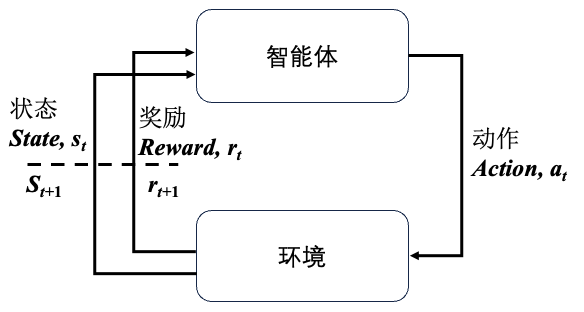
\includegraphics[width=0.6\textwidth]{figure/chapter1/强化学习.png}
    \caption{\label{fig:rlcontrol}强化学习控制回路}
\end{figure}

强化学习的目标是最大化智能体在整个交互过程中获得的累积奖励。当环境的动态满足马尔可夫性质,即下一状态仅依赖于当前状态和所采取的行动时,
这个过程可以被建模为一个马尔可夫决策过程(MDP)。

马尔可夫决策过程提供了一个框架来形式化描述智能体的行为和环境的反应,通常由$\left \langle S,A,P,\gamma,R \right \rangle$五元组构成。
其中,$P$表示状态转移概率方程,$p\left(s^{\prime} \mid s, a\right)$
表达在状态s,动作a下过渡到新状态$s^{'}$;$\gamma$表示折扣因子,其反映了对当前奖励和未来奖励的权衡。$pi$通常表示智能体的策略,是状态映射到动作的
函数,$\pi(a|s)$表示在状态$s$中选择动作$a$的概率,轨迹$\tau$是交互过程中产生MDP元组的集合。因此强化学习的目标函数为:
\begin{align}
        J(\pi)=\underset{\tau \sim \pi }{\mathrm{E}}\left [ R(\tau) \right ]=\underset{\tau \sim \pi }{\mathrm{E}}\left[\sum_{t=0}^{\infty} \gamma^{t} R_{t}\right]
\end{align}

为了解决这一优化目标,强化学习引入了价值函数。值函数一般可以分为动作值函数和状态值函数,它们被用来评估智能体在给定状态(或给定状态与动作)下有多“好“
(由回报的期望值定义),有助于智能体了解在预期的后续回报方面各个状态和动作的关联程度。
在策略$\pi$下状态$s$的价值函数,动作值函数和优势值函数被定义为:
\begin{align}
    V^{\pi}\left(s\right) & = \mathbb{E}_{\pi }\left[\sum_{k = 0}^{\infty} \gamma^{k} R_{t+k+1}\mid S_{t}= s\right]\\
    Q^{\pi}\left(s, a\right) &=\mathbb{E}_{\pi }\left[\sum_{k = 0}^{\infty} \gamma^{k} R_{t+k+1}\mid S_{t}= s,A_{t}=a\right]\\
    A^{\pi}(s, a)&=Q^{\pi}(s, a)-V^{\pi}(s)
\end{align}

然而,实际应用中的强化学习问题往往伴随着各种约束,如安全、资源和操作限制等。这些约束条件的存在要求我们在追求奖励最大化的同时,也需要确保智能体的行为不会违
反这些约束。这就引出了受限马尔可夫决策过程(Constrained MDP, CMDP)的概念,它在普通的MDP框架上增加了成本(Cost)概念,以模拟在满足任务目标的同时遵守约束的需要。
\begin{align}
    \text{Cost} & = \mathbb I(d(s,a,s')>0)\\
    \text{s.t.} \ &d(s,a,s')\le 0 \notag
\end{align}
其中d为约束的具体表达形式。

类似的,可以获得成本价值函数$V_{c}$与成本动作值函数$Q_{c}{s,a}$以及轨迹成本的期望值$J_{c}(\pi)$。
\begin{align}
    V^{\pi}_{c}\left(s\right) & = \mathbb{E}_{\pi }\left[\sum_{k = 0}^{\infty} \gamma^{k} C_{t+k+1}\mid S_{t}= s\right]\\
    Q^{\pi}_{c}\left(s, a\right) &=\mathbb{E}_{\pi }\left[\sum_{k = 0}^{\infty} \gamma^{k} C_{t+k+1}\mid S_{t}= s,A_{t}=a\right]\\
    A^{\pi}_{c}(s, a)&=Q^{\pi}_{c}\left(s, a\right)-V^{\pi}_{c}\left(s\right)\\
    J_{c}(\pi)&=\underset{\tau \sim \pi }{\mathrm{E}}\left[\sum_{t=0}^{\infty} \gamma^{t} C_{t}\right]
\end{align}
\subsubsection{算法原理及训练流程}
近端策略优化(Proximal Policy Optimization, PPO)\cite{schulman2017proximal}算法被广泛认为是最有效的同策略优化方法。PPO基于于单调策略改进定理,有效确保了策略收敛的稳定性,并且在面对强化学习中的约束问题
时,PPO能够通过结合拉格朗日乘子和对偶梯度下降将约束优化问题转化为无约束优化问题。基于这些特性,我们采用了结合拉格朗日乘子法的PPO算法(PPO-Lagrange,PPOLag)来优化无人机逆过渡问题。
定义优化问题如下,其中$d_{i}$表示为对应约束的成本阈值,通常表示为一回合内容许违反约束次数的上限:
\begin{align}
    &\max _{\pi \in \Pi_{\theta}} J_{R}(\pi) \\
    &\text { s.t. } J_{C_{i}}(\pi) \leq d_{i},\forall i \notag
\end{align}

由单调策略改进定理可知:
\begin{align}
    J\left(\pi^{\prime}\right)-J(\pi) & =\mathbb{E}_{s_{0}}\left[V_{\pi^{\prime}}\left(s_{0}\right)\right]-\mathbb{E}_{s_{0}}\left[V_{\pi}\left(s_{0}\right)\right] \\ \notag
    & =\mathbb{E}_{\pi^{\prime}}\left[\sum_{t=0}^{\infty} \gamma^{t} r\left(s_{t}, a_{t}\right)\right]+\mathbb{E}_{\pi^{\prime}}\left[\sum_{t=0}^{\infty} \gamma^{t}\left(\gamma V_{\pi}\left(s_{t+1}\right)-V_{\pi}\left(s_{t}\right)\right)\right] \\ \notag
    & = \mathbb{E}_{\pi^{\prime}}\left[\sum_{t=0}^{\infty} \gamma^{t} A_{\pi}\left(s_{t}, a_{t}\right)\right] \notag
\end{align}
其中,$\pi^{\prime}$表示新策略,$\pi$表示旧策略。通过优化新旧策略之差,可以保证策略单调改进。但由于无法利用尚未更新的新策略去收集样本从而求解问题,因此PPOLag算法基于新旧策略分布差异较小的约束假设,进行了一定的近似:
\begin{align}
    J\left(\pi^{\prime}\right)-J(\pi)
    &=  \mathbb{E}_{\tau \sim \pi^{\prime}}\left[\sum_{t=0}^{\infty} A^{\pi}\left(s_{t}, a_{t}\right) \right]\\ \notag
    &\approx \mathbb{E}_{\tau \sim \pi}\left[\sum_{t=0}^{\infty} A^{\pi}\left(s_{t}, a_{t}\right) \frac{\pi^{\prime}\left(a_{t}|s_{t}\right)}{\pi\left(a_{t}|s_{t}\right)}\right]=J_{\pi}^{CPI}(\pi^{\prime})\\
    J_{C_{i}}\left(\pi^{\prime}\right)-J_{C_{i}}(\pi)
    &=  \mathbb{E}_{\tau \sim \pi^{\prime}}\left[\sum_{t=0}^{\infty} A_{C_{i}}^{\pi}\left(s_{t}, a_{t}\right) \right]\\ \notag
    &\approx \mathbb{E}_{\tau \sim \pi}\left[\sum_{t=0}^{\infty} A_{C_{i}}^{\pi}\left(s_{t}, a_{t}\right) \frac{\pi^{\prime}\left(a_{t}|s_{t}\right)}{\pi\left(a_{t}|s_{t}\right)}\right]=J_{C_{i},\pi}^{CPI}(\pi^{\prime})
\end{align}
其中,$C_{i}$表示智能体的第$i$个约束,等式表达式即为新旧策略之间的性能差异,通过优化新旧策略差异下界即可从而最大化新策略的性能指标保证非负改进,但由于等式中的期望值需要从新策略$\pi^{\prime}$中进行采样更新,
但新策略$\pi^{\prime}$却需要在更新之后才可以获得。

为了解决这一矛盾。TRPO中提出了保守策略迭代(Conservative policy iteration,CPI)下的近似目标函数,即在新旧策略相对接近(一般用KL散度约束)能够保证其状态访问分布相似的前提下,
使用旧策略的轨迹$\tau \sim \pi$结合重要性采样定理来替换原本的目标函数。
同时由于最终的目标是优化策略参数网络参数$\theta$,优化目标变为:
\begin{align}
    J^{CPI}(\theta) = \mathbb{E}_{t}\left[ A_{t}^{\pi_{\theta_{old}}} \frac{\pi_{\theta}\left(a_{t}|s_{t}\right)}{\pi_{\theta_{old}}\left(a_{t}|s_{t}\right)}\right] & = \mathbb{E}_{t}\left[r_{t}(\theta)A_{t}\right]\\
    J_{C_{i}}^{CPI}(\theta) = \mathbb{E}_{t}\left[ A_{C_{i},t}^{\pi_{\theta_{old}}} \frac{\pi_{\theta}\left(a_{t}|s_{t}\right)}{\pi_{\theta_{old}}\left(a_{t}|s_{t}\right)}\right] & = \mathbb{E}_{t}\left[r_{t}(\theta)A_{C_{i},t}\right]
\end{align}

优化问题变为如下:
\begin{align}
\begin{split}
    &\theta_{k+1} = \mathop{\arg\min}\limits_{\theta} \underset{\substack{\tau \sim \pi_{k}}}{\mathbb{E}}\left[-r(\theta) A_{R}^{\pi_{k}}(s, a)\right] \\
    &\text { s.t. } J_{C_{i}}(\pi_{k})+\underset{\substack{\tau \sim \pi_{k}}}{\mathbb{E}}\left[r(\theta) A_{C_{i}}^{\pi_{k}}(s, a)\right] \leq d_{i} \quad \forall i \\
    &\bar{D}_{K L}\left(\pi^{\theta_{k+1}} \| \pi^{\theta_{k}}\right) \leq \delta 
    \label{prime}
\end{split}
\end{align}
由于PPOLag会使用裁剪目标函数来保证KL散度的约束,因此,暂时将KL散度约束忽略,使用拉格朗日松弛技术将原本的约束优化问题,转化为无约束优化问题:
\begin{align}
\begin{split}
    \theta^{*}&=\min _{\theta} \max _{\lambda_{i} \geq 0} L(\theta, \lambda_{i}),\\
        \textit{} {with}\ L(\theta,\lambda_{i}) & = \left [r(\theta)(-A_{R}^{\pi_{k}}(s, a)+ \sum_{i}^{m} \lambda_{i}A_{C_{i}}^{\pi_{k}}(s, a))\right ]\\
        &+ \sum_{i}^{m} \lambda_{i}(J_{C_{i}}(\pi_{k})-d_{i})
\end{split}
\label{lag}
\end{align}

根据\cite{tessler2018reward}中的理论,此时优化的目标是找到\autoref{lag}问题中的鞍点$(\theta^{*}(\lambda^{*}),\lambda^{*})$。
此时的拉格朗日乘子可以被认为是一个惩罚系数,也可以被认为是奖励与惩罚的自动权衡系数。随着违反约束的不可行惩罚项增大,不可行解会变为次优解,
因此随着拉格朗日乘子的增大,\autoref{lag}的解会收敛于\autoref{prime}中的解。

因此可以采用双时间尺度方法去轮流更新策略网络参数$\theta$和拉格朗日乘子$\lambda_{i}$,
其中,策略网络参数通常要求快速更新,以保证算法快速适应或探索环境;拉格朗日乘子参数通常要求以较慢的学习率更新,直到约束被满足,
这是因为快速变化的拉格朗日乘子会导致违反约束的惩罚项变化过于激烈,从而导致算法不稳定。

在双尺度更新的更新下,\autoref{lag}的最小最大问题,可以被分为两个独立的问题,考虑\autoref{lag}外层的最小化问题:
\begin{align}
    \underset{\theta}{\operatorname{minmize}} \ \underset{\tau \sim \pi_{k}}{\mathbb{E}}\left[r(\theta)(-A_{R}^{\pi_{k}}(s, a)+ \sum_{i}^{m} \lambda_{i}A_{C_{i}}^{\pi_{k}}(s, a))\right]
\end{align}
其中,$d_{i}$是成本阈值,$J_{C_{i}}(\pi_{k})$是旧策略的累计折扣成本,因此$J_{C_{i}}(\pi_{k})-d_{i}$是常数,并不影响策略梯度更新,因此可以被忽略。
同时为了保证更新的稳定性,对优势函数进行简单归一化:
\begin{align} 
    {A}_{\lambda^{\prime}}^{\pi_{k}}(s, a)&=\frac{-A_{R}^{\pi_{k}}(s, a)+ \sum_{i}^{m} \lambda_{i}A_{C_{i}}^{\pi_{k}}(s, a)}{1+\sum_{i}^{m} \lambda_{i}} 
\end{align}

在解决策略参数$\theta$的KL散度约束时, PPO为了避免求解KL散度引入的额外运算复杂度,使用裁剪的方式对目标函数进行一阶优化,
当策略更新偏离原始策略太多时,这个函数会对这些更新进行裁剪,以维护更新的稳定性并极大的加快了训练速度,由于裁剪掉的样本不能够产生梯度
裁剪也提供了一定的训练稳定性,裁剪后的目标函数变为:
\begin{align} 
    L^{C L I P}(\theta) & = \underset{\tau \sim \pi_{k}}{\mathbb{E}}\left[\min \left(r(\theta) {A}_{\lambda^{\prime}}^{\pi_{k}}(s, a), \operatorname{clip}\left(r(\theta), 1-\epsilon, 1+\epsilon\right) {A}_{\lambda^{\prime}}^{\pi_{k}}(s, a)\right)\right]
    \label{aloss}
\end{align}

同样的,只考虑影响拉格朗日乘子更新项。\autoref{lag}中内层的最大化问题为:
\begin{align}
    \underset{\lambda}{\operatorname{maxmize}} \ \underset{\tau \sim \pi_{k}}{\mathbb{E}}\left[\sum_{i}^{m} \lambda_{i}\left[(J_{C_{i}}(\pi_{k})-d_{i})+r(\theta)A_{C_{i}}^{\pi_{k}}(s, a)\right]\right]
\end{align}    
其中,策略更新的目标函数能够用被有效的裁剪,从而保证新旧策略足够“接近”,
因此可以假设$ \underset{\tau \sim \pi_{k}}{\mathbb{E}}\left[A_{C_{i}}^{\pi_{k}}(s, a)\right]= 0$\cite{zhang2020first}。
在实际更新时,每个约束i对应的$\lambda_{i}$的更新方式为:
\begin{align}
    \lambda_{i} \leftarrow \underset{\lambda_{i}}{\operatorname{proj}}\left[\lambda_{i}-\alpha\left(d_{i}-J_{C_{i}}(\pi_{k})\right)\right]
\end{align}
其中,$\alpha$表示步长,投影算子的目的是为了将拉格朗日乘子限制在$\left [ 0,\lambda_{max} \right ] $中,以保证策略稳定。
除此之外,PPOLag算法为了更好的评估优势值函数,采用了广义优势估计方法,公式如下:
\begin{align}
    \widehat{A}_{t}^{G A E(\gamma, \lambda)} = \sum_{l = 1}^{\infty}(\gamma \lambda)^{l} \delta_{t+l}^{V} = \sum_{l= 1}^{\infty}(\gamma \lambda)^{l}\left(r_{t}+\gamma V\left(s_{t+l+1}\right)-V\left(s_{t+l}\right)\right)
\end{align}
综上PPOLag算法的伪代码如下所示:
\begin{algorithm}[H]
    \begin{algorithmic}[1] % enter the algorithmic environment
        \STATE \textbf{初始化}:随机初始化策略网络 $\pi_{\theta_{0}}$, 值函数网络 $V_{R}^{\phi_{0}}$, 成本值函数网络 $V_{C}^{\psi_{0}}$,$\forall i$, 迭代更新次数$N$
        \FOR{$k$ in $0,1,2, \ldots, K$}
        \STATE 使用策略$\pi_{\theta_{k}}$与无人机环境进行交互,运行$T$步收集轨迹$\tau$
        \STATE 根据奖励$R$,使用GAE估计优势值函数$\hat{A}_{R}^{\pi_{\theta_{k}}}\left(s_{t}, a_{t}\right)$,并计算$V_{tar}^{\phi_{k}}\left(s_{t}\right)=\hat{A}_{R}^{\pi_{\theta_{k}}}\left(s_{t}, a_{t}\right)+\hat{V}_{R}^{\pi_{k}}(s_{t})$
        \STATE 根据约束成本$C$,使用GAE估计优势值函数$\hat{A}_{C_{i}}^{\pi_{\theta_{k}}}\left(s_{t}, a_{t}\right)$,$\forall i$,计算$V_{C,tar}^{\phi_{k}}\left(s_{t}\right)=\hat{A}_{C_{i}}^{\pi_{\theta_{k}}}\left(s_{t}, a_{t}\right)+\hat{V}_{C}^{\pi_{k}}(s_{t})$
            \FOR{$i$ in $0,1,2, \ldots, N$}
                \FOR{each minibatch}
                    \STATE \textbf{更新拉格朗日乘子}:$\lambda_{i}^{k+1} \leftarrow \underset{\lambda_{i}}{\operatorname{proj}}\left[\lambda_{i}^{k}+\alpha\left(J_{C_{i}}(\pi_{k})-d_{i}\right)\right]$
                    \STATE \textbf{更新Critic网络}:$\phi_{k+1}=\arg \min _{\phi}\text{MSE}\left(V_{R}^{\phi_{k}}\left(s_{t}\right)-V_{tar}^{\phi_{k}}\left(s_{t}\right)\right)^{2}$
                    \STATE \textbf{更新CostCritic网络}:$\psi_{k+1}=\arg \min _{\psi}\text{MSE}\left(V_{C}^{\psi_{k}}\left(s_{t}\right)-V_{C,tar}^{\psi_{k}}\left(s_{t}\right)\right)^{2}$
                    \STATE \textbf{计算ActorLoss} 根据 \autoref{aloss}
                    \STATE \textbf{更新Actor网络}:$\theta \leftarrow \theta-\eta \nabla L^{C L I P}(\theta)$
                \ENDFOR
            \ENDFOR
        \ENDFOR
        \STATE \textbf{输出}:策略网络参数$\theta$
    \end{algorithmic}
    \caption{\label{alg:ppolag}PPOLag算法}
\end{algorithm}
\subsection{强化学习环境设计}
\label{chapter:env}
强化学习中状态空间、动作空间设置如下:
\begin{equation}
    \begin{aligned}
    s &= \left(u,w,\sin \theta , \cos \theta , q, v_{x},v_{z}\right)^{T} \in R^{7}, \\
    a &= \left(\delta_{y},\omega_{r}\right)^{T} \in R^{2}.
    \end{aligned}
\end{equation}
其中,状态量包括机体坐标系和地面坐标系下的速度以及角度信息。角度的相关信息采用正余弦变换后的俯仰角去表征,这是因为正余
弦变换能够有效地编码方向信息和提供更稳定的数值属性。
而动作空间选定为经过归一化后的
螺旋桨转速和舵面偏转,取值范围为[-1,1],当输出实际动作时,会根据动作的最大值和最小值进行放缩和平移。
奖励与成本函数设置如下:
\begin{gather}
    \Phi (s_{t})=k_{1}\sqrt{v_{x}^{2}+v_{z}^{2}}+k_{2}\left | \theta-\pi/2 \right | \\\notag
    Reward=\kappa(\left | u \right | < 0.5 \ \text{and}\ \left | w \right | < 0.5\ \text{and}\ \left | \theta \right | < 5^{\circ}\ \text{and}\ \left | q \right | < 5^{\circ})\\ \notag
    +(\Phi (s_{t+1})-\Phi (s_{t}))\times (0.99)^{t/10}\\ \notag
    Cost=\mathbb I(max(\left | V_{z} \right |-0.4,\left | q \right |-\pi/2 )>0)  \notag
\end{gather}
其中,$\kappa=100,k_{1}=1,k_{2}=10$,奖励与成本函数分析如下:
\begin{itemize}
    \item [1.] $\kappa$ 是对成功完成过渡的奖励也称终端奖励,通常是一个较大的数值。这样的奖励函数从密度上比较稀疏(只有一步可以得到),给探索造成了很大难度,
    但可以提供精准的描述任务需求,拥有较强的鲁棒性。期望累计回报则可以近似为
    $\underset{\tau \sim \pi }{\mathrm{E}}\left[\sum_{t=0}^{\infty} \gamma^{t}\kappa\right]$, 
    由于折扣因子通常小于1,因此最大化期望累积回报也可以被认为是在最小化过渡任务完成时间。成功过渡的定义同\autoref{tab:constraints},终端状态量需满足指定约束。
    \item [2.] $\Phi (s_{t})=k_{1}\sqrt{v_{x}^{2}+v_{z}^{2}}+k_{2}\left | \theta-\pi/2 \right |$是一种经典的奖励重塑(reward-shaping)形式,$\Phi (s_{t})$
    在这里表示势能函数,可以将无人机朝期望目标状态引导,起到为智能体“导航”的作用,本质上是一种稠密奖励,起到辅助智能体的作用,
    其系数$(0.99)^{t/10}$有两层直观的物理意义:1. 它表示奖励函数会随着时间而逐步衰减符合我们期望时间最短的目标。2. 它表示随着离期望目标状态越近,辅助奖励所占据的比重
    越小,减小辅助奖励可能带来的负面影响。
    \item [3.] 成本函数采用指示函数,当角速度约束和垂向速度约束任一被违背时,cost为1,否则为0。通过max函数将两个约束转化为一个约束,相应的约束阈值d设为0,以保证逆过渡过程中
    约束零违反。
\end{itemize}

环境状态转移设置如下:无人机环境状态转移可以由\autoref{eq:three_dof}中的动力学方程提供,同时为了精准描述环境状态转移,本文中一律采用四阶龙格库塔法进行仿真,
设无人机动力学模型为:$x_{t+1}=f\left(x_{t}, u_{t}\right)$,状态转移方程如下:
\begin{align}
    x_{t+1}&=x_{t}+\frac{\tau}{6}\left(k_{1}+2 k_{2}+2 k_{3}+k_{4}\right)\\
    k_{1} & =f\left(x_{t}, u_{t}\right) \\
    k_{2} & =f\left(x_{t}+\tau \frac{k_{1}}{2},u_{t}\right) \\
    k_{3} & =f\left(y_{n}+\tau \frac{k_{2}}{2}, u_{t}\right) \\
    k_{4} & =f\left(y_{n}+\tau k_{3}, u_{t}\right)
\end{align}
其中,$\tau$为仿真步长,取0.2s。
综上,我们在$Open AI gym$中注册了我们的涵道无人机环境,以便后续强化学习算法的开发。
% \subsection{课程学习}
% 快速定高过渡的难点在于如何在高度变化较小的条件下更快地消耗无人机动能。因此随着初始俯仰角的减小,初始水平速度会增加,无人机的初始动能更大从而加大了快速定高过渡问题的难度。
% 而强化学习算法中初始状态通常采用均匀分布随机化(Uniform Distribution Randomization, UDR),此时算法会更加注重智能体的平均性能表现,可能会收敛在局部最优。
% 为了避免这种情况的实现,我们采用课程学习(Curriculum Learning, CL)\cite{bengio2009curriculum}设计一系列难度逐渐加大的任务去训练智能体,以保证智能体在不同的初始条件下拥有良好
% 的性能表现。例如:我们可以令无人机从最简单的初始角度15°开始进行训练,当无人机在目前的初始条件下过渡成功率达到100\%且过渡过程中零违反约束时,初始角度会相应的减小1°,否则会一直在
% 当前初始条件训练。具体的伪代码如下:
% \begin{algorithm}[H]
%     \begin{algorithmic}[1] % enter the algorithmic environment
%         \STATE \textbf{输入}:初始俯仰角$\theta_{t_{0}}=\theta_{t_{0}}^{max}$,初始策略$\pi_{0}$        
%         \FOR{$k$ in $0,1,2, \ldots, K$}
%         \STATE 指定环境初始状态分布$\rho_{k} \leftarrow Unif(\theta_{k}-1,\theta_{k}+1)$
%         \STATE 根据\autoref{alg:ppolag}的3-14行,训练策略$\pi_{k} \leftarrow trainpolicy(\rho_{k},\pi_{k-1})$
%         \STATE 评估当前策略 $success \ rate,epcost \leftarrow evalpolicy(\pi_{k},\rho_{k})$
%         \IF{$success \ rate \ is \ 100 \% \ and \  epcost \ is \ 0$}
%             \STATE $\theta_{t_{0}} = max(\theta_{t_{0}} - 1,\theta_{t_{0}}^{min})$
%         \ELSE
%             \STATE $\theta_{t_{0}} = min(\theta_{t_{0}},\theta_{t_{0}}^{max})$
%         \ENDIF
%         \ENDFOR
%         \STATE \textbf{输出}:策略网络参数$\theta$
%     \end{algorithmic}
%     \caption{\label{alg:CL}课程学习}
% \end{algorithm}
\section{实验仿真与结果分析}
本节采用了Intel(R) Xeon(R) Gold 5220 CPU 2.20GHz 18核心和NVIDIA GeForce 2080TI GPU进行训练。
在评估过程中,为了确保算法评估的公正性,实验结果会取每一回合的24次平均性能。其中,初始俯仰角从4°变化到15°,间隔为0.5°,
以确保覆盖各种任务难度。训练相关的超参数如下:
\begin{table}[H]
    \centering
    \caption{\label{tab:algoconfig}PPOLag算法超参数}
    \begin{tabularx}{0.7\linewidth}{|c|X|c|}
        \hline
        参数 & 参数说明 & 参数值 \\ \hline
        steps per epoch & 一回合交互步数 & 12000 \\ \hline
        update iters & 一回合更新次数 & 10 \\ \hline
        batch size & 批处理容量 & 64 \\ \hline
        entropy coef & 熵损失系数 & 0.01 \\ \hline
        max grad norm & 梯度裁剪阈值 & 40.0 \\ \hline
        critic norm coef & 价值函数正则项 & 0.001 \\ \hline
        gamma & 折扣因子 & 0.99 \\ \hline
        lam & 广义优势估计参数 & 0.95 \\ \hline
        clip & 裁剪比 & 0.2 \\ \hline
        std & 策略分布方差 & $[0.1,0.5]$ \\ \hline
        feature dim & 策略/价值神经网络隐藏层 & $[128,128]$ \\ \hline
        activation & 激活函数 & tanh \\ \hline
        learning rate & 学习率 & 0.0003 \\ \hline
        cost limit & 成本阈值 & 0.0 \\ \hline
        lag init & 拉格朗日乘子初值 & 0.01 \\ \hline
        lag learning rate & 拉格朗日乘子学习率 & 0.035 \\ \hline
    \end{tabularx}
\end{table}


本章共进行了三组实验。首先,对比了PPOLag算法和使用固定惩罚因子的PPO算法的性能表现,并进行了过渡轨迹对比,
以验证PPOLag算法中拉格朗日乘子的必要性;
然后与总能量控制算法以及基于伪谱法的GPOPS-II软件所求解的逆过渡轨迹进行了对比,突显了本文方法的有效性;
最后,对不同初始条件下的无人机进行蒙特卡洛逆过渡飞行实验仿真,统计了无人机逆过渡性能指标。

\subsection{模型训练结果与对比}
为了说明拉格朗日的重要作用,进行了PPOLag算法与PPO结合固定惩罚系数的对比实验,其中,PPO中的奖励函数被重构为$R\left(s, a, s^{\prime}\right)-p C\left(s, a, s^{\prime}\right) \text { for } p \in\{1,5,10\}$,
$p$表示惩罚因子大小,实验效果如\autoref{fig:PPOLag_and_FPO_comparison}所示。

可以看出PPO算法对于惩罚系数的选取非常敏感,当$\nu=1$时,PPO算法会在获得较大奖励但同时违反约束一定次数;当$\nu=5$时,PPO算法的违反约束次数会快速降低至0,但比起PPOLag,
算法的收敛速度会显著降低,最终的累计奖励也略低于PPOLag算法;当$\nu=10$时,同样地,PPO算法的违反约束次数会快速降低至0,但其也会因此没有学会如何获得奖励,甚至在200-300回合时,PPO-10会出现
成本函数波动的情况,这是因为智能体缺乏正样本的引导,只能不断地加大模型的探索力度,导致训练不稳定。而PPOLag算法在训练过程中,会自动选择惩罚系数,以实现奖励与约束成本之间的理想权衡。
其过渡轨迹对比如\autoref{fig:lagcmp}:

可以发现由于缺乏合适的惩罚因子,PPO算法在逆过渡问题上表现不佳,当惩罚因子过小时,无人机会经常违反约束设定,学会类似连续上升这类损失高度的过渡方法;而惩罚因子过大时,
无人机经常会学习到保守的策略,增大过渡时间,甚至有可能无法学会任何有效信息,只是一直保持水平飞行($p=10$)。

综上,在解决类似逆过渡这类在训练初期会频繁违反约束的强化学习问题时,PPOLag算法相较于PPO算法可以通过逐渐增大的拉格朗日乘子,保证最后的约束满足,同时,又可以避免训练初期的
惩罚力度过大影响到智能体的探索,不仅减少了强化学习复杂的奖励函数调整,同时无需对奖励和约束成本的规模进行调整,因为此时拉格朗日乘子可以自动帮助算法完成调整。
\begin{figure}[H]
    \centering
    \subfloat[奖励函数曲线]{% 创建子图(a)
        \includegraphics[width=0.48\linewidth,height=0.4\linewidth]{chapter3/reward_three_comparison.png}
        \label{fig:reward_cmp3}
    }
    \hfill % 使两个子图间有空隙
    \subfloat[成本函数曲线]{% 创建子图(b)
        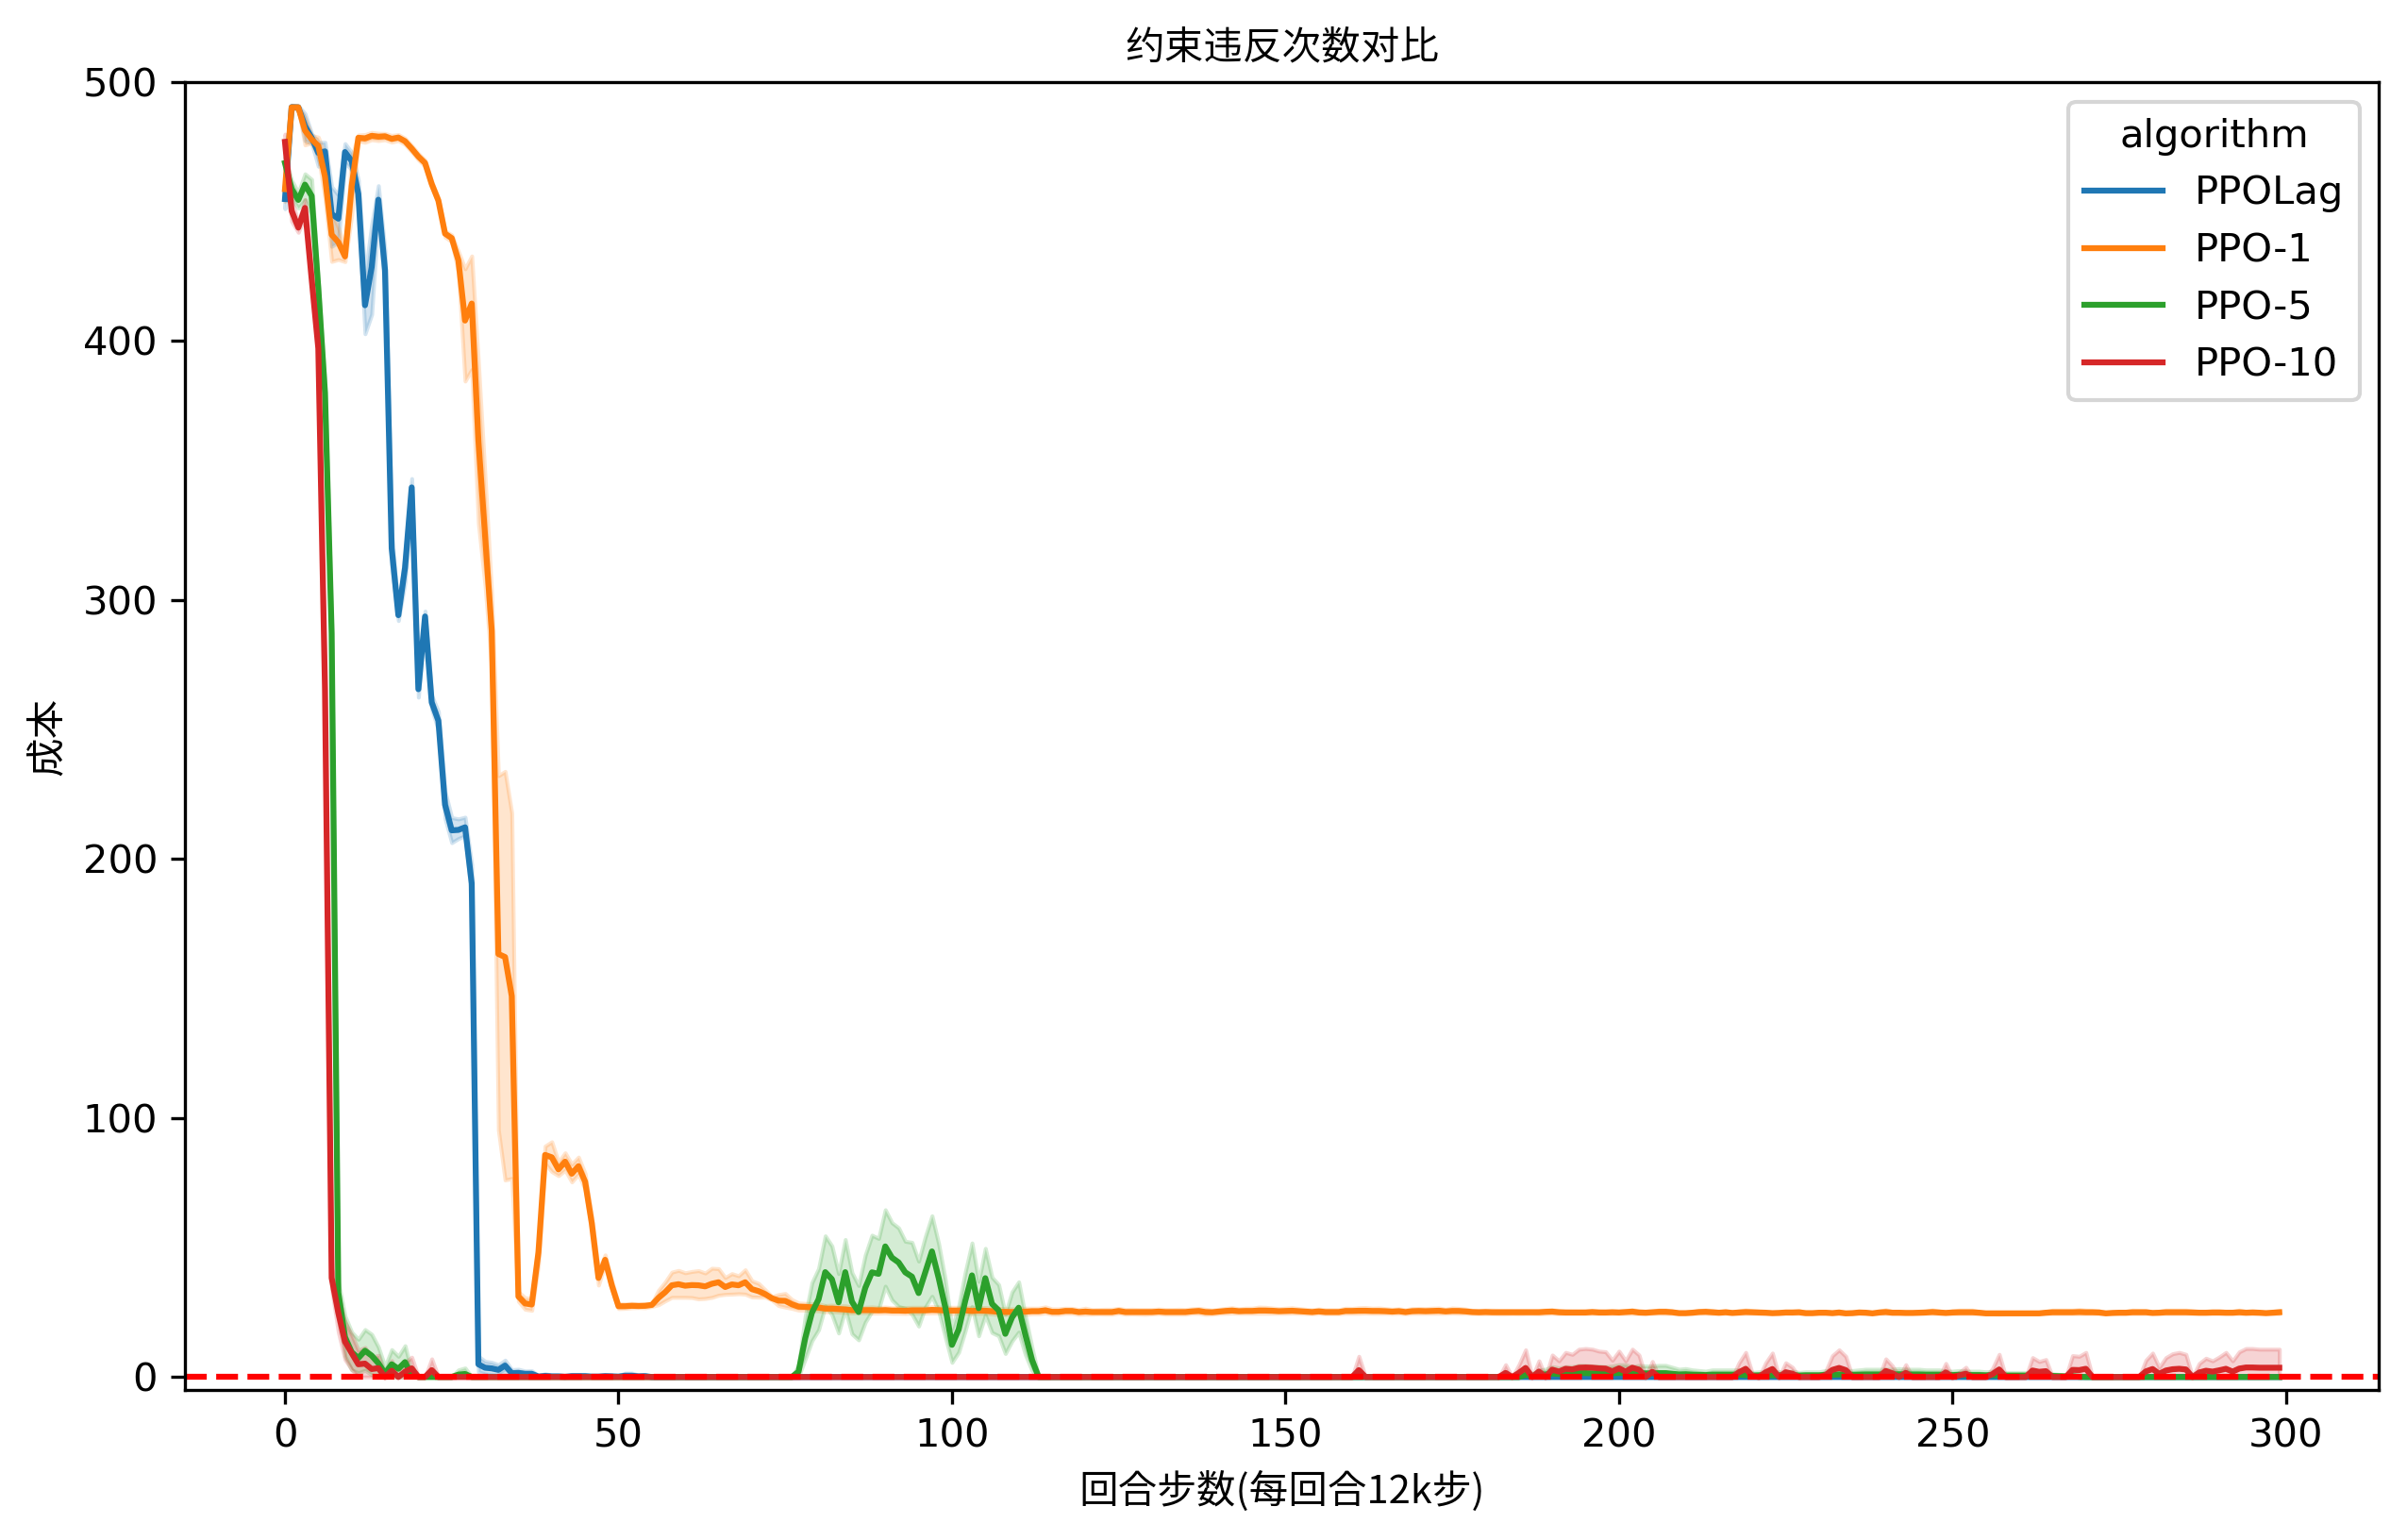
\includegraphics[width=0.48\linewidth,height=0.4\linewidth]{chapter3/cost_three_comparison.png}
        \label{fig:cost_cmp3}
    }
    \caption{PPOLag与固定惩罚系数的PPO性能对比} % 创建整个图形的主标题和标签
    \label{fig:PPOLag_and_FPO_comparison}
\end{figure}
\begin{figure}[H]
    \centering
    % 第一行
    \begin{subfigure}{.45\textwidth}
        \centering
        \includegraphics[width=1.1\linewidth]{chapter3/lag/Vx.png}
        \caption{水平速度}
        \label{fig:vxcmp}
    \end{subfigure}%
    \hfill % 在子图之间添加一些空间
    \begin{subfigure}{.45\textwidth}
        \centering
        \includegraphics[width=1.1\linewidth]{chapter3/lag/Vz.png}
        \caption{垂向速度}
        \label{fig:vzcmp}
    \end{subfigure}
    % 换行,开始第二行
    \\
    % 第二行
    \begin{subfigure}{.45\textwidth}
        \centering
        \includegraphics[width=1.1\linewidth]{chapter3/lag/Theta.png}
        \caption{俯仰角}
        \label{fig:vxcmp}
    \end{subfigure}%
    \hfill % 在子图之间添加一些空间
    \begin{subfigure}{.45\textwidth}
        \centering
        \includegraphics[width=1.1\linewidth]{chapter3/lag/q.png}
        \caption{俯仰角速率}
        \label{fig:vzcmp}
    \end{subfigure}
    % 添加整体标题和标签
    \caption{拉格朗日乘子与固定惩罚系数过渡轨迹对比}
    \label{fig:lagcmp}
\end{figure}

% \subsection{课程学习与均匀分布初始化对比}
% \begin{figure}[htbp]
%     \centering
%     \begin{minipage}{.7\linewidth}
%         \centering
%         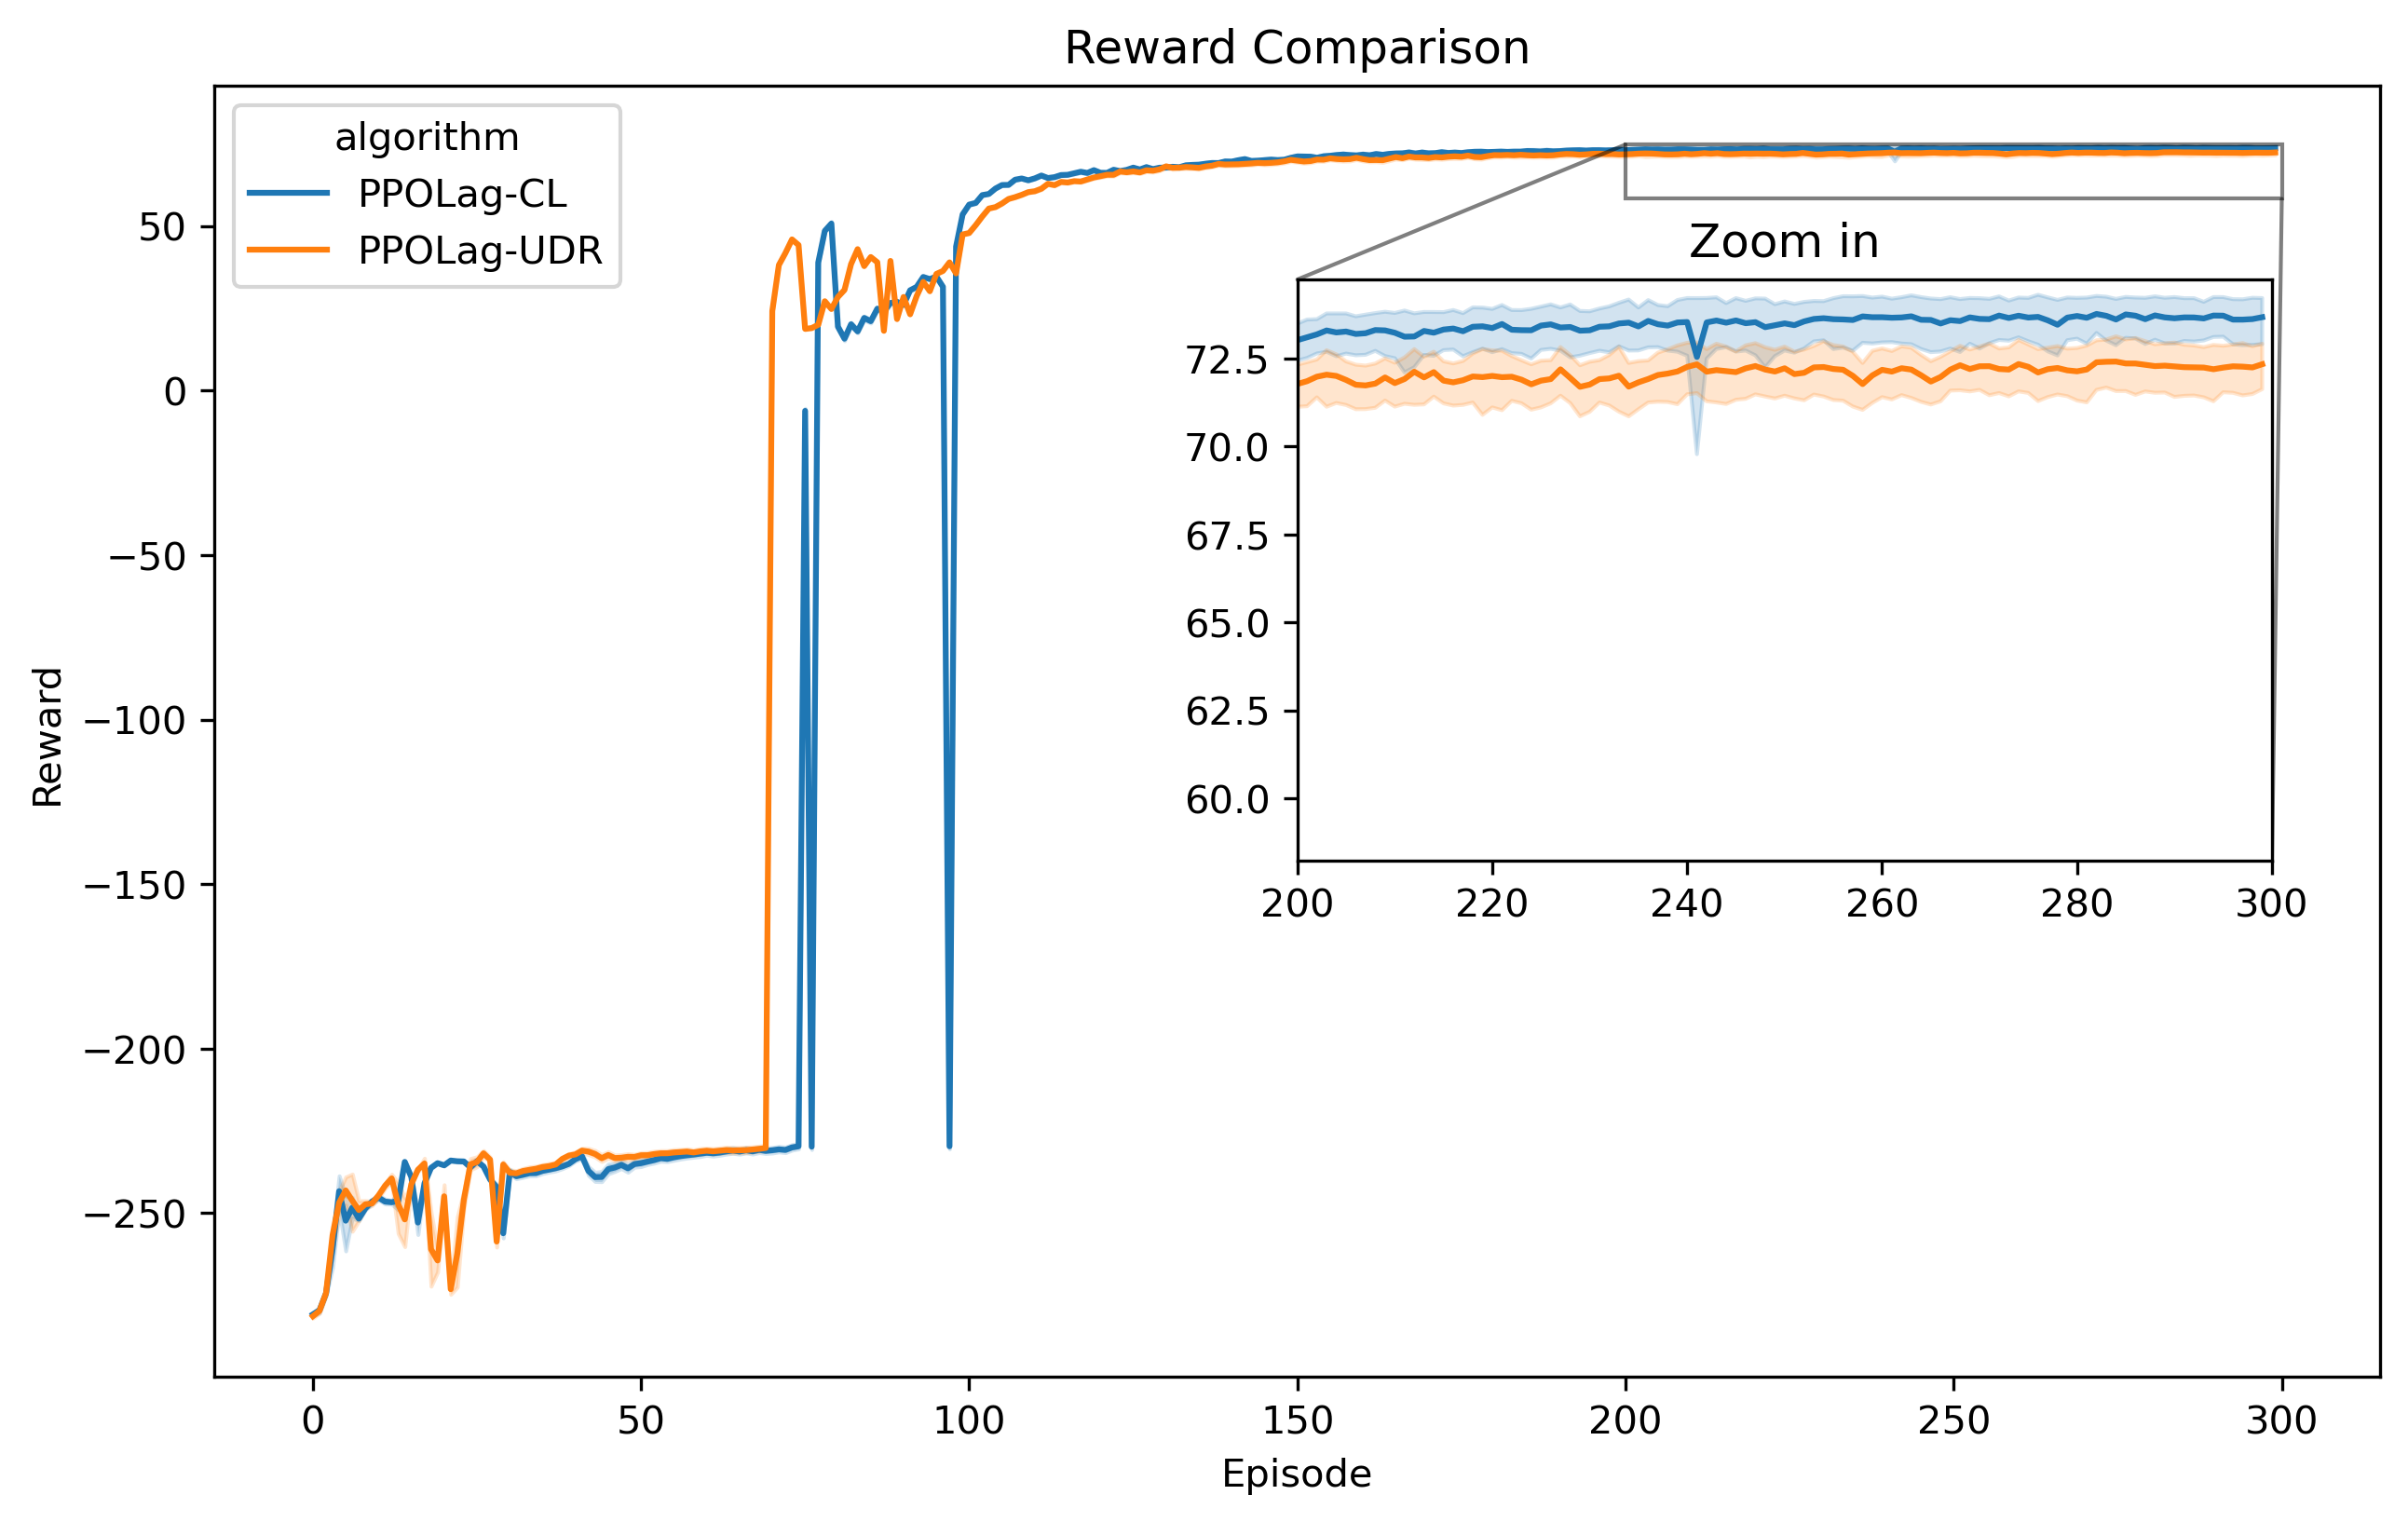
\includegraphics[width=\linewidth]{chapter3/reward_comparison_with_zoom.png}
%         \caption{奖励函数曲线}
%         \label{fig:reward_cmp}
%     \end{minipage}
%     \begin{minipage}{.7\linewidth}
%         \centering
%         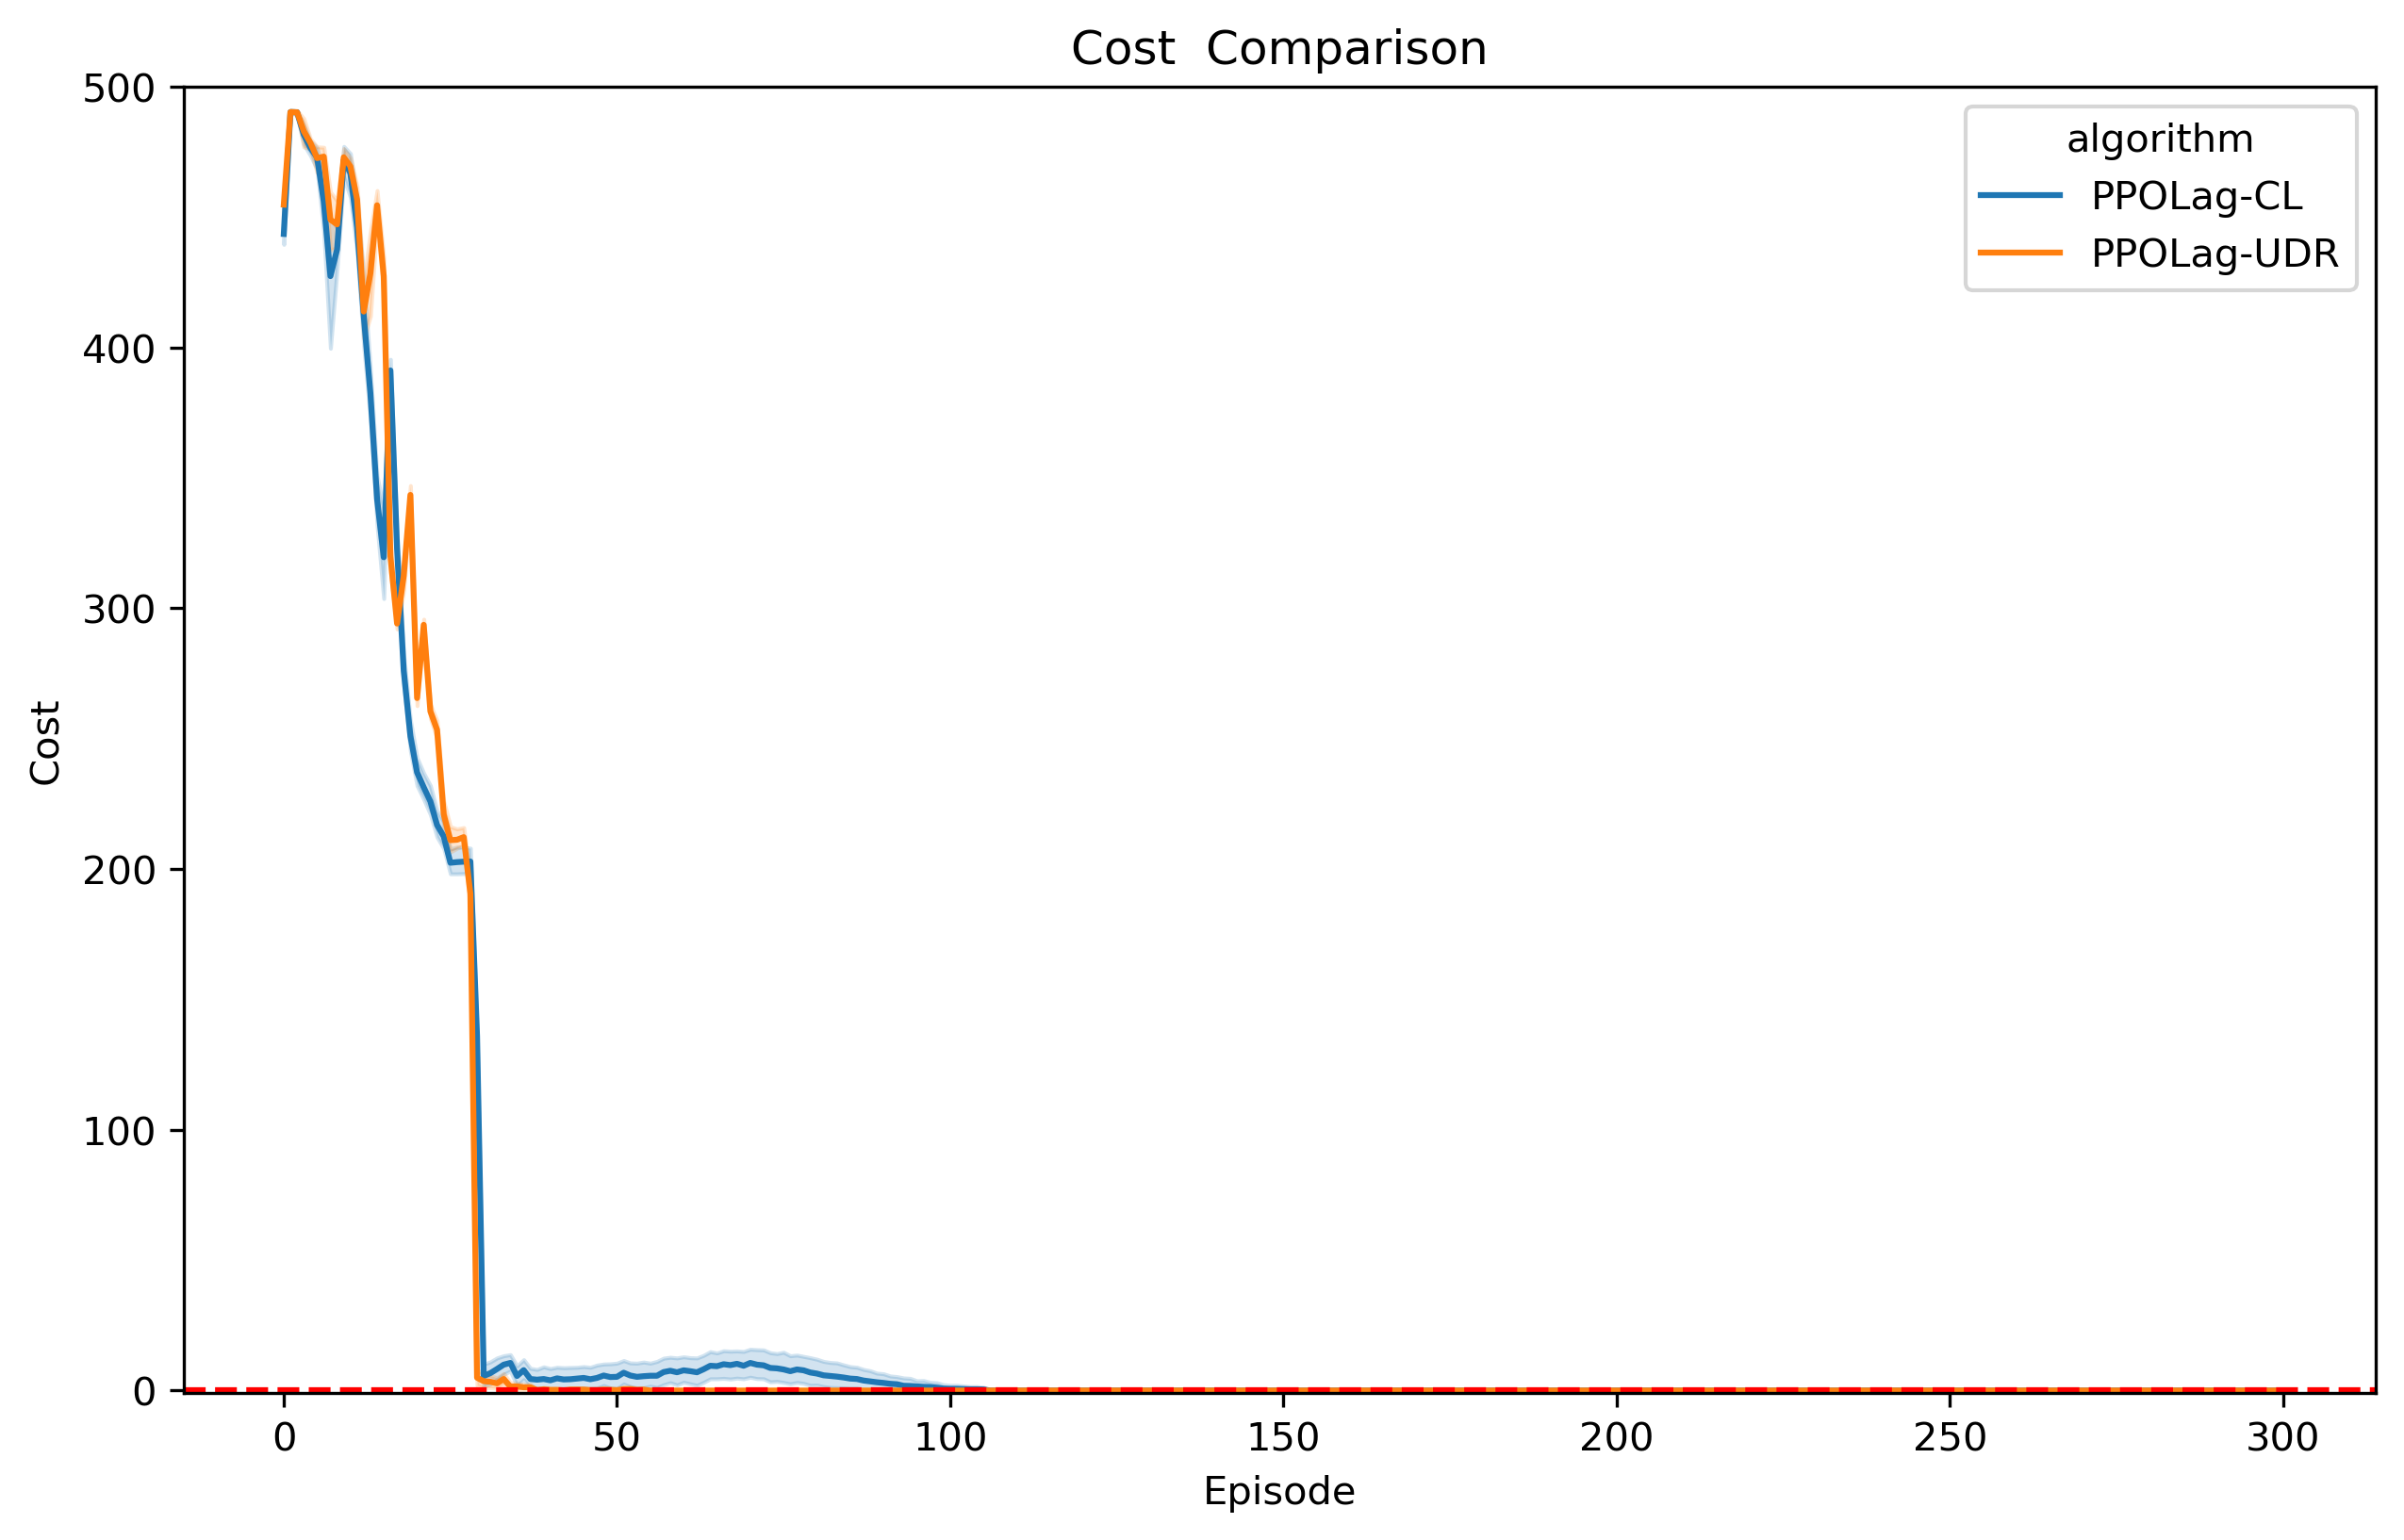
\includegraphics[width=\linewidth]{chapter3/cost_comparison.png}
%         \caption{成本函数曲线}
%         \label{fig:cost_cmp}
%     \end{minipage}
%     \caption{课程学习和均匀分布初始化对比}
%     \label{fig:UDR_and_CL_comparison}
% \end{figure}
% 由图可以看出,在训练过程中,使用课程学习的指定课程进行初始化相较于UDR初始化最终收敛的策略相对更优,从任务难度角度来说,UDR优化的是不同初始分布下累计回报的期望,
% 而CL则是在100-300回合时会专注于优化难度最大的初始分布下的累计回报期望,在忽略潜在的智能体“性能遗忘”的条件下,这提供了更好的性能表现。
\subsection{与其它过渡方法对比}
总能量控制系统(Total Energy Control System,简称TECS)是一种用于常用于尾座式无人机飞行控制的系统。TECS的核心是通过控制无人机的俯仰角(升降舵)和油门,调整飞机的动能和势能的平衡。
这种方法可以在变化的飞行条件下通过调整动能和势能的变化,以达到期望的高度和速度,从能量角度出发处理了无人机飞行过程中高度和速度的耦合问题。同时由于过渡过程中,传统的TECS
控制方案难以适用于悬停状态,因此本文采用了\cite{argyle2016modeling}中改进的TECS控制系统去执行涵道无人机的过渡控制进行对比。

TECS需要根据人工先验设计期望的速度曲线,在经由TECS进行控制,因此,选择初始俯仰角为4°,设定期望水平加速度为-3m/s,期望垂向速度为0。控制效果如下:
\begin{figure}[htbp]
    \centering
    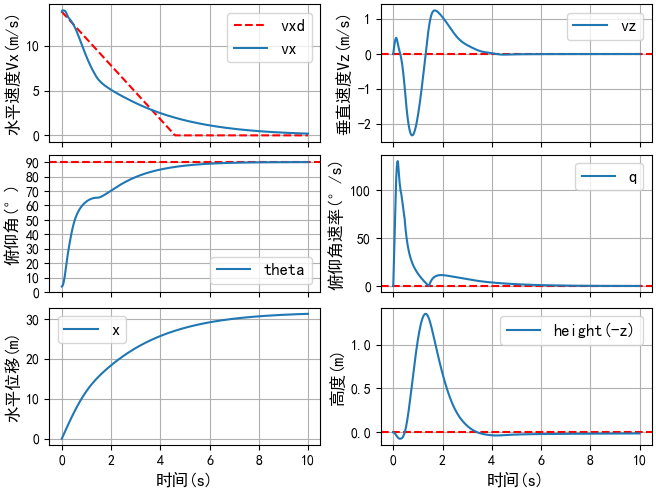
\includegraphics[width=0.9\textwidth]{chapter3/tecs.png}
    \caption{\label{fig:tecs}总能量控制系统控制效果}
    \label{fig:tecs}
\end{figure}
\autoref{fig:tecs}展示了TECS控制下的逆过渡过程。可以观察到,逆过渡所需时间接近10秒,垂向速度最大误差达到2.3米/秒,角速度最大达到130°,
高度最大变化达到1.35米,同时水平速度存在较大的控制误差。

TECS设计简单,仅需简单的PID控制器就可以完成逆过渡控制。
然而,与PPOLag算法相比,其过渡时间过长,同时无法满足约束,过渡过程中高度变化较大,过渡性能较差。实验发现,
进一步减小期望水平加速度的值并不会缩短其过渡时间,
这也进一步说明了期望速度曲线的设计难点。

根据\cite{cheng2022transition}的研究,涵道无人机在实现定高转换的逆过渡过程中,
水平速度的变化也会带来水平加速度约束范围的变化。
因此,凭借经验手动设计的期望速度曲线很难保证无人机完成定高转换过渡。
相比之下,强化学习算法可以通过试错的方式自行探索出合理的飞行包线。

\subsubsection{与最优控制对比}

% 由3.2节可知,无人机逆过渡轨迹优化问题也可被视为最优控制算法进行求解。因此,本文采用非线性规划软件GPOPS-II\cite{patterson2014gpops}进行求解。GPOPS-II采用直接法中的自适应Radau伪谱法,
% 使用Legendre-Gauss-Radau点作为离散配点,基于MATLAB平台实现。

如第3.2节所述,无人机逆过渡轨迹优化问题可以采用最优控制方法进行求解。
据此,本研究选用了高级非线性规划工具GPOPS-II\cite{patterson2014gpops}进行轨迹优化。
该软件实现了自适应Radau伪谱法,其利用Legendre-Gauss-Radau点进行离散化,基于MATLAB平台实现。
\begin{figure}[htbp]
    \centering
    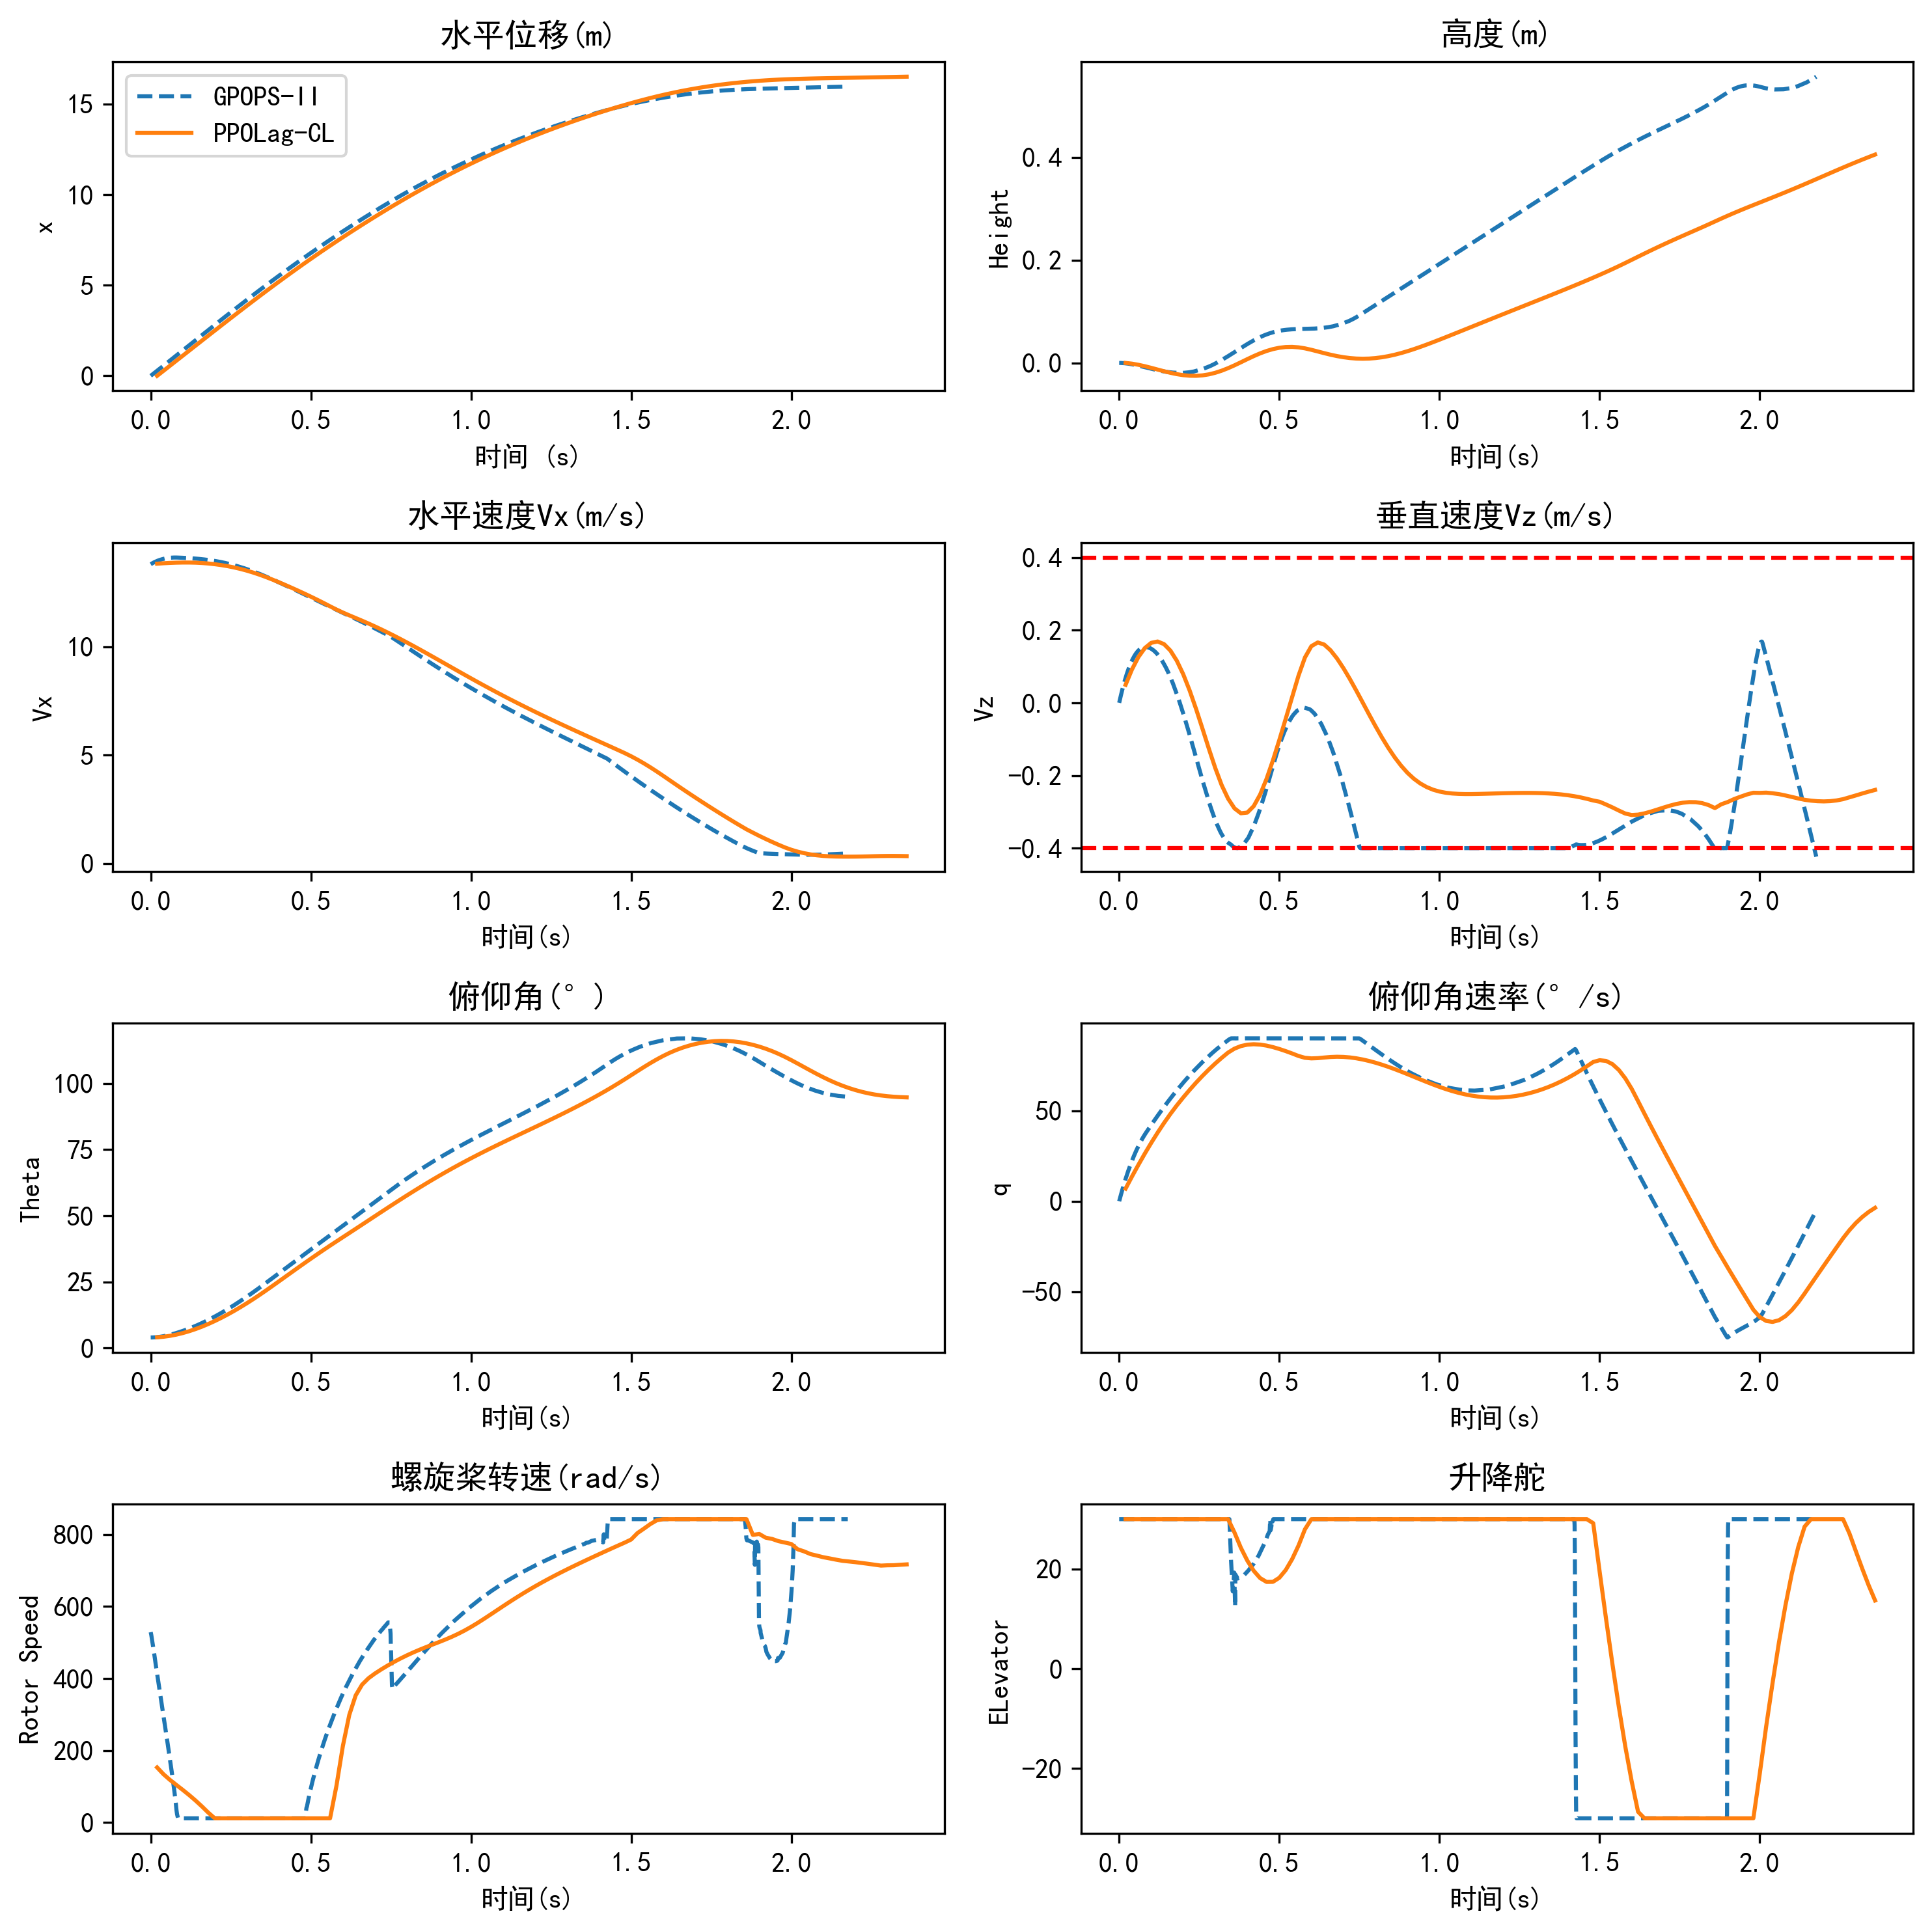
\includegraphics[height=16cm,width=0.8\textwidth]{chapter3/gpopsvsrl.png}
    \caption{\label{fig:gpops}GPOPS-II vs RL}
    \label{fig:gpops}
\end{figure}

在采用GPOPS-II解决无人机逆过渡控制策略的问题时,类似于强化学习,本研究同样纳入了无人机的动力学模型,
并选取了螺旋桨转速及舵机偏转角度作为控制变量。
本小节共利用GPOPS-II进行了两组实验,分别是:直接优化产生的逆过渡飞行轨迹;
和将GPOPS-II计算得到的螺旋桨转速和俯仰角指令作为输入,
实施了前馈-比例积分微分(PID)控制策略\cite{verling2017model}的飞行轨迹,其中控制框图如\autoref{fig:gpopstheme}。
\begin{figure}[H]
    \centering
    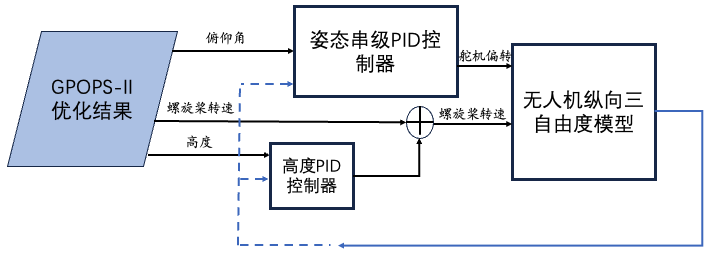
\includegraphics[height=4cm,width=0.8\textwidth]{chapter3/gpops2.png}
    \caption{\label{fig:gpopstheme}结合GPOPS-II的过渡控制结构}
    \label{fig:gpops}
\end{figure}

仿真结果如\autoref{fig:gpops}所示。当初始角度为4°时,GPOPS-II所求解的最优轨迹过渡时间为2.18秒,结合控制后的过渡时间为2.4秒,
而PPOLag的过渡时间为2.36秒。在GPOPS-II求解的过渡过程中,高度最大变化为0.56米,结合控制后高度最大变化为0.79米,而PPOLag的高度最大变化为0.40米。
可以观察到,PPOLag算法所求解的最优轨迹与GPOPS-II直接优化的结果十分接近,比结合GPOPS-II的前馈PID控制过渡性能更好。
同时可以观察到,结合了PID和前馈控制后,其过渡性能会因执行器的响应滞后而存在一定的性能下降,导致过渡性能下降,无法满足约束。

与基于GPOPS-II的逆过渡轨迹相比,PPOLag其垂直速度与俯仰角速率约束距离约束边界会保留一定的裕度。
更重要的是,GPOPS-II求解的控制量变化剧烈,而PPOLag算法所求解的控制量则相对更加光滑,更适合作为真实执行器的输入。

GPOPS-II利用伪谱法把最优控制问题转化为非线性规划(NLP)问题,并依据Karush-Kuhn-Tucker(KKT)条件来解决受约束的优化问题。
由此得到的优化轨迹一般展示出优异的性能特征。
然而,该优化求解过程计算量庞大,通常难于在机载嵌入式系统中达到实时求解。

在实际应用中,习惯将优化后的轨迹预先存储于计算机系统中,并在离线状态下进行执行,这一策略对于轨迹优化的鲁棒性提出了更高要求。
与之对照,PPOLag等强化学习算法在处理现实世界的不确定因素及模型误差时,显示出更加出色的适应性和鲁棒性。
更容易应对真实世界的干扰和模型不匹配的情况。

\subsection{纵向逆过渡飞行实验}
为了验证飞行数据的有效性,随机初始化无人机水平飞行状态,在水平飞行1秒钟后,
进行60次蒙特卡洛逆过渡模态转换仿真实验。仿真结果如\autoref{fig:mcflight_all}所示。
% \paragraph{位移和速度仿真结果}
\begin{figure}[H]
    \centering
    \begin{subfigure}{.46\textwidth}
        \centering
        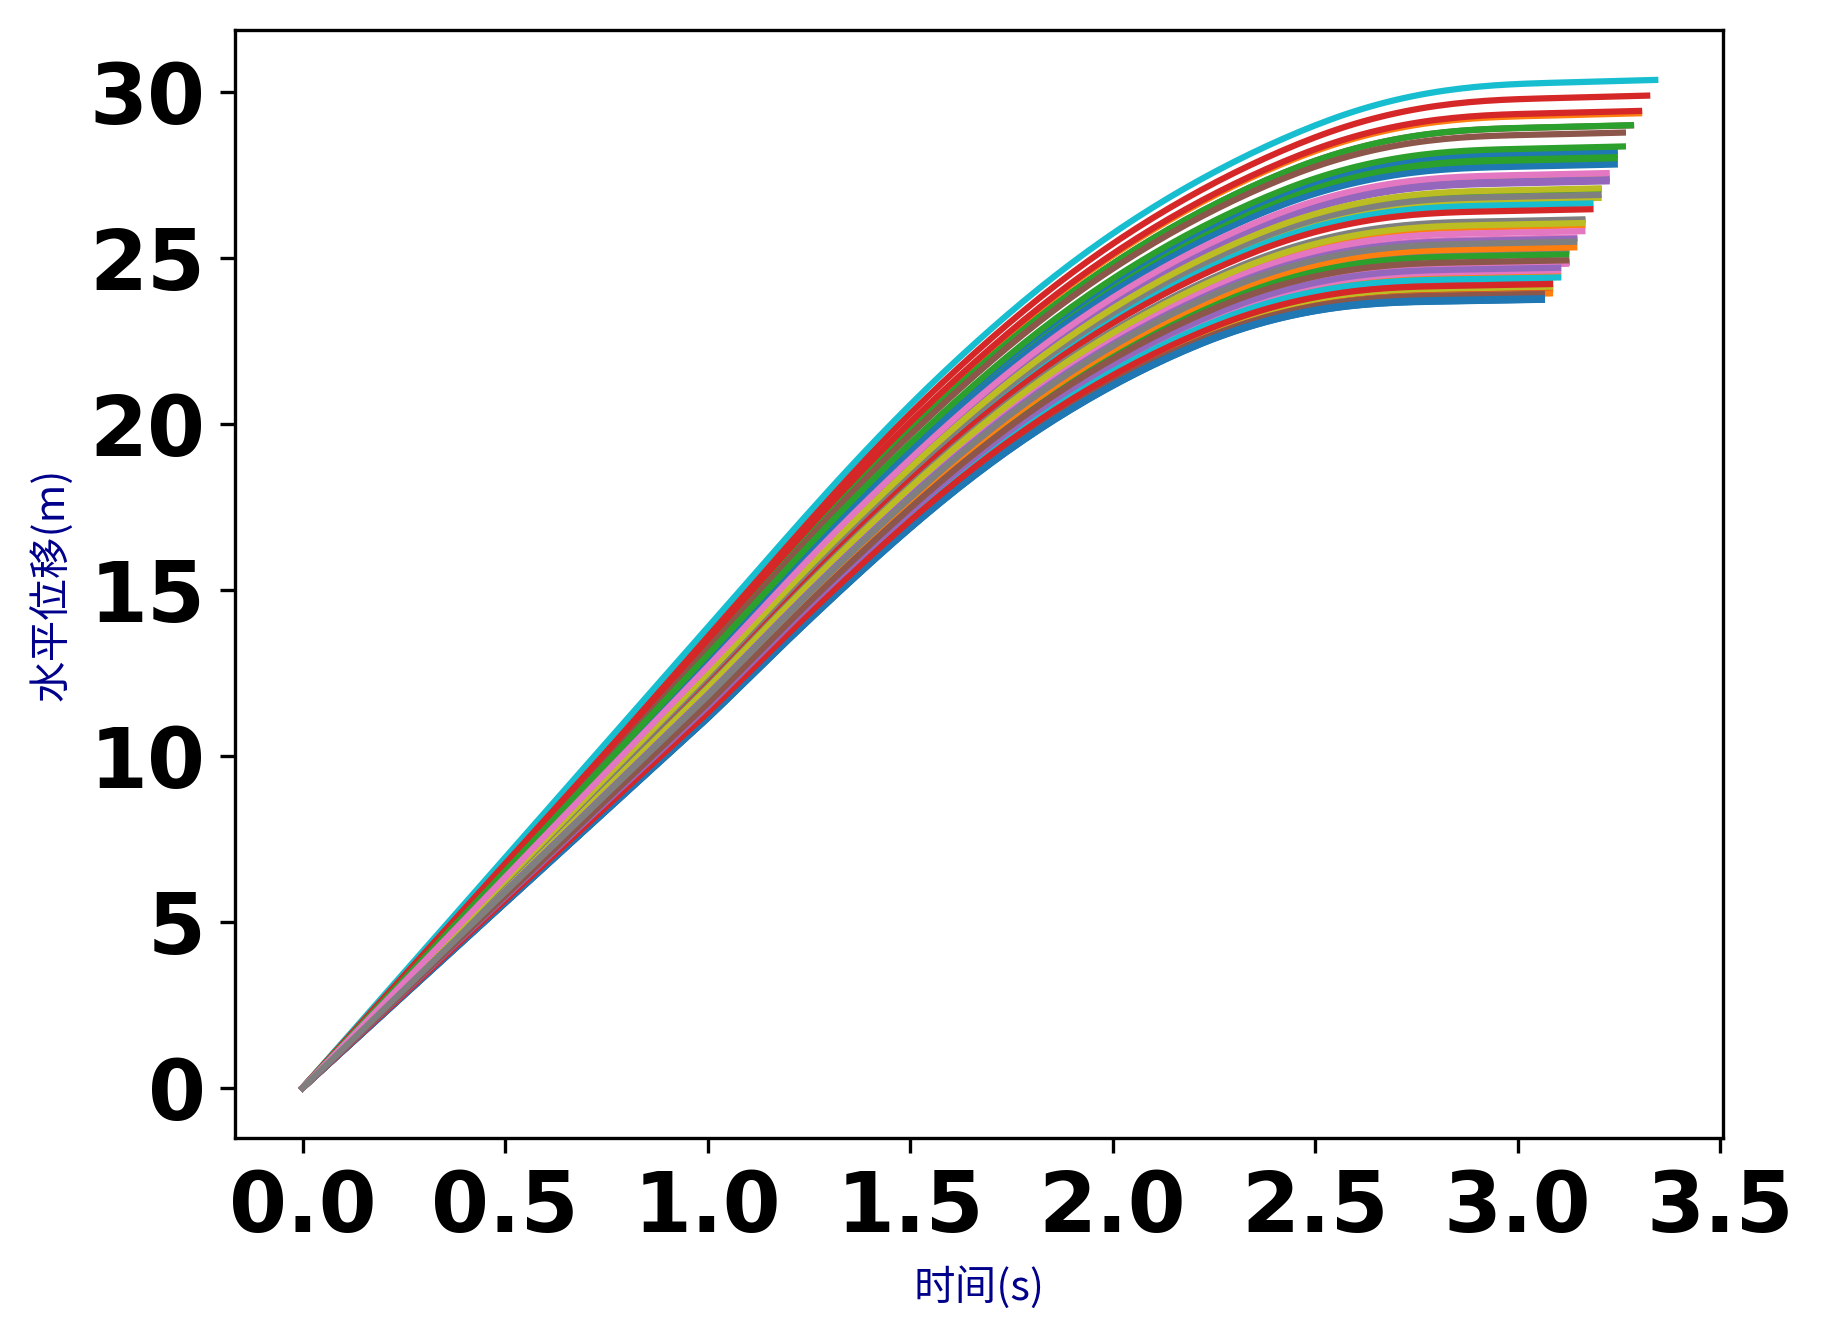
\includegraphics[width=\linewidth]{chapter3/x.png}
        \caption{横向位移}
        \label{fig:sub1}
    \end{subfigure}% <-- 注意这里的百分号
    \begin{subfigure}{.46\textwidth}
        \centering
        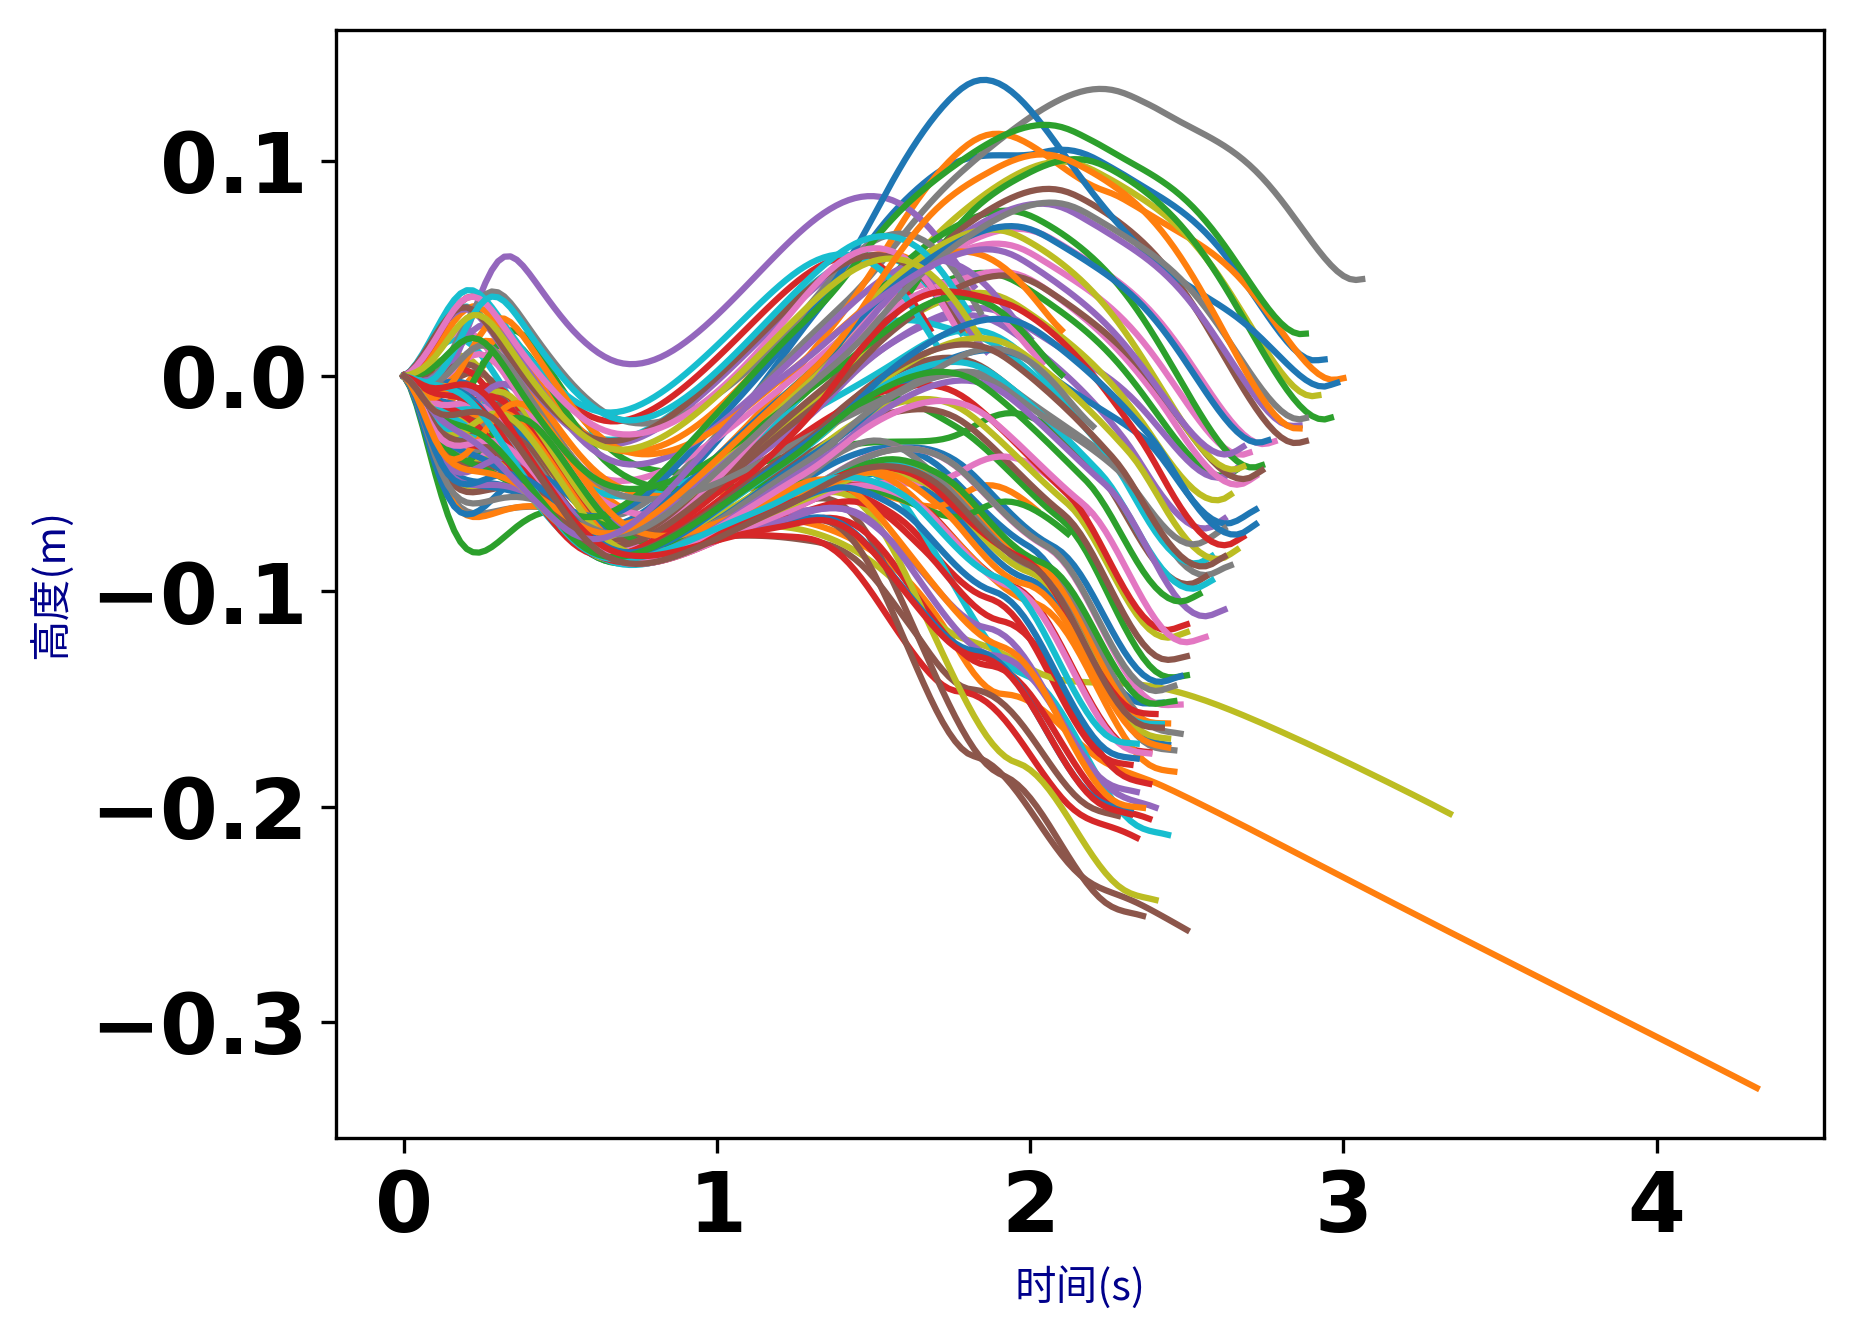
\includegraphics[width=\linewidth]{chapter3/height.png}
        \caption{垂直位移}
        \label{fig:sub2}
    \end{subfigure}
    \begin{subfigure}{.46\textwidth}
        \centering
        \includegraphics[width=\linewidth]{chapter3/Vx.png}
        \caption{横向速度}
        \label{fig:sub3}
    \end{subfigure}% <-- 注意这里的百分号
    \begin{subfigure}{.46\textwidth}
        \centering
        \includegraphics[width=\linewidth]{chapter3/Vz.png}
        \caption{垂直速度}
        \label{fig:sub4}
    \end{subfigure}
    \begin{subfigure}{.46\textwidth}
        \centering
        \includegraphics[width=\linewidth]{chapter3/Theta.png}
        \caption{俯仰角}
        \label{fig:sub5}
    \end{subfigure}% <-- 注意这里的百分号
    \begin{subfigure}{.46\textwidth}
        \centering
        \includegraphics[width=\linewidth]{chapter3/q.png}
        \caption{俯仰角速率}
        \label{fig:sub6}
    \end{subfigure}
    \begin{subfigure}{.46\textwidth}
        \centering
        \includegraphics[width=\linewidth]{chapter3/ele.png}
        \caption{升降舵偏转}
        \label{fig:sub7}
    \end{subfigure}% <-- 注意这里的百分号
    \begin{subfigure}{.46\textwidth}
        \centering
        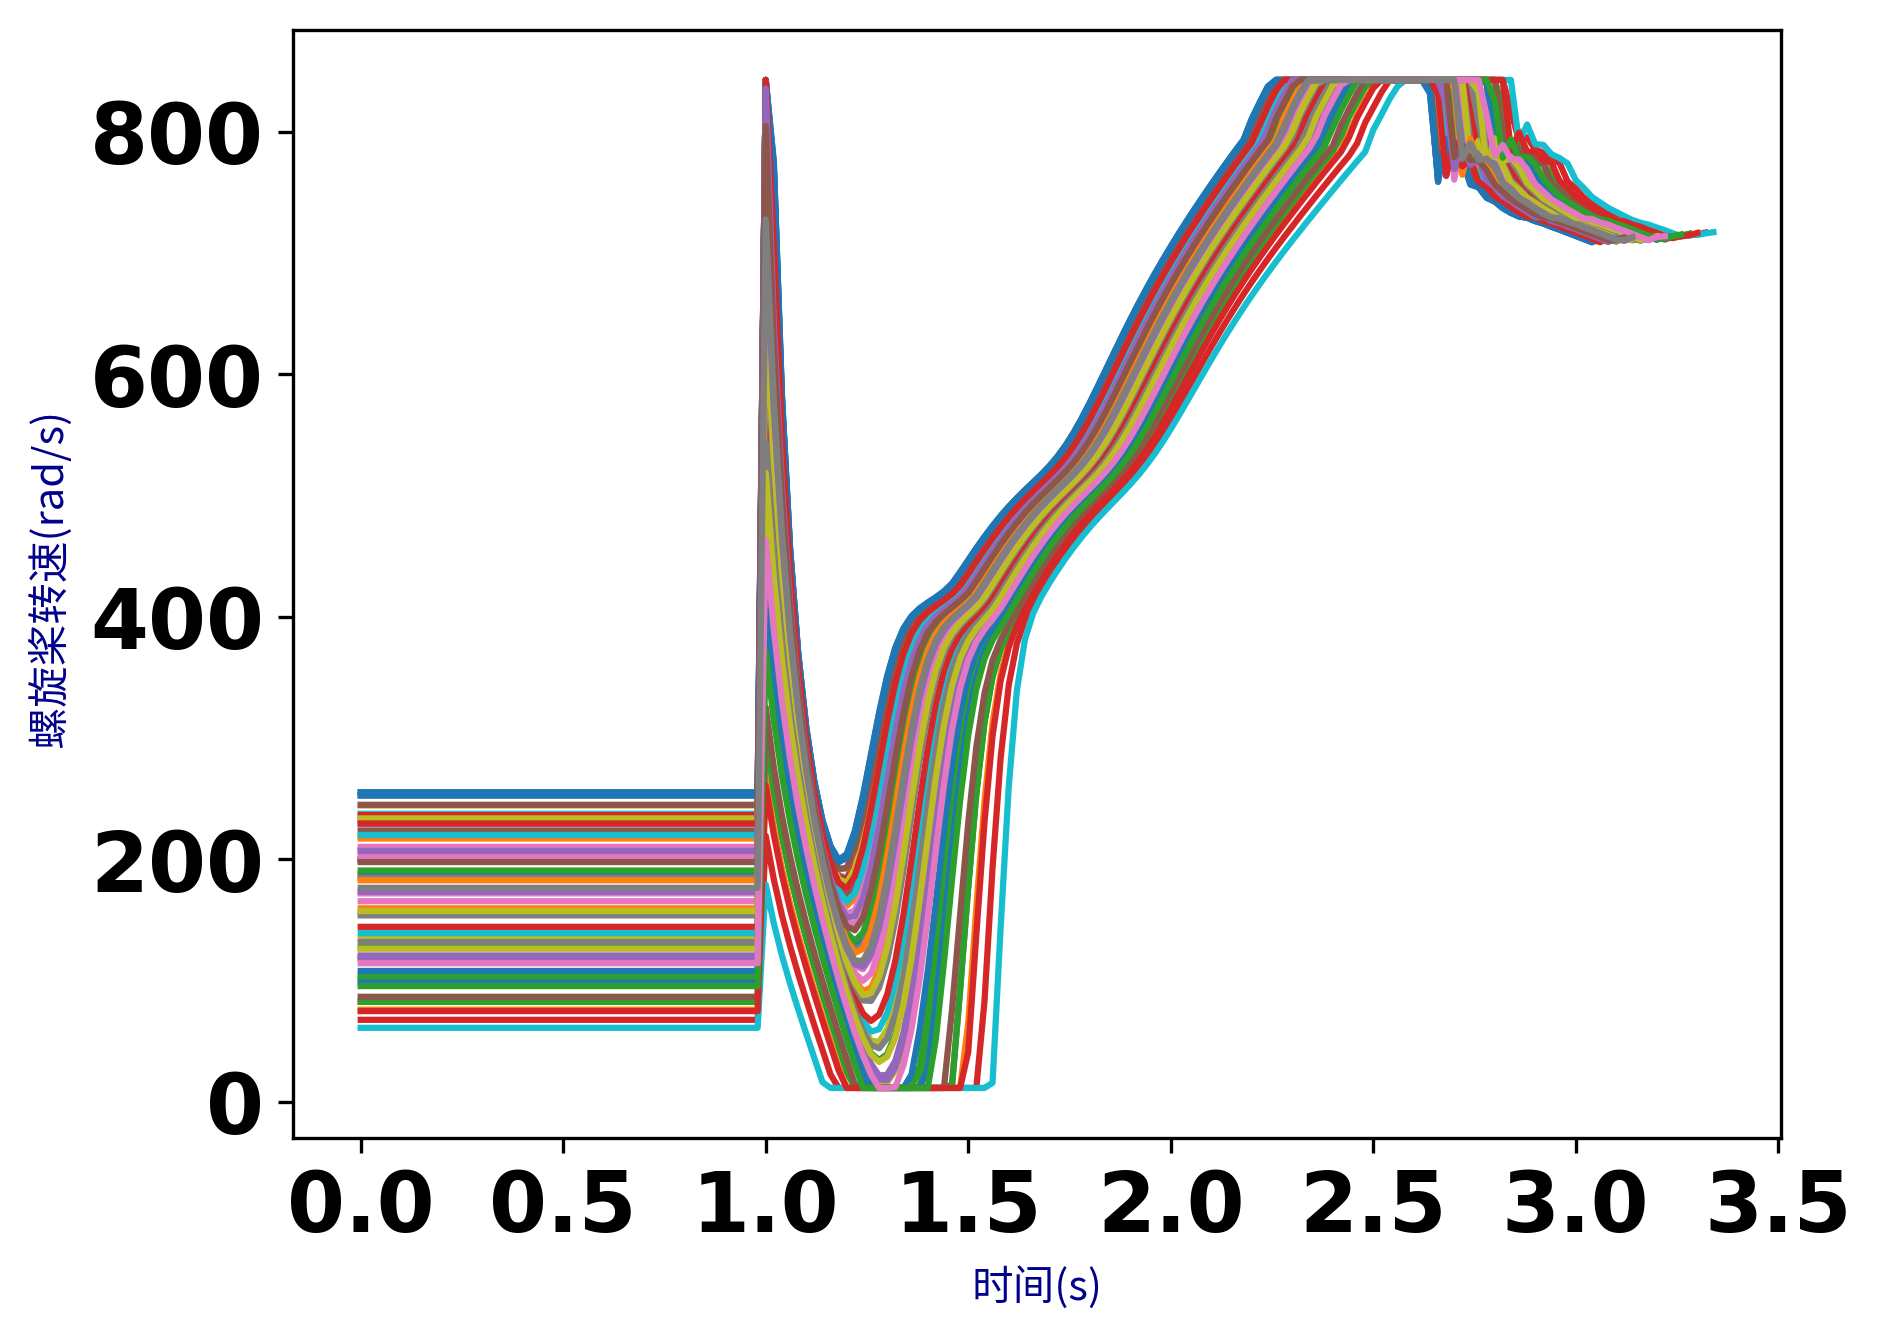
\includegraphics[width=\linewidth]{chapter3/speed.png}
        \caption{螺旋桨转速}
        \label{fig:sub8}
    \end{subfigure}
    \caption{逆过渡位移、速度、姿态和控制输入示意图}
    \label{fig:mcflight_all}
\end{figure}

仿真数据表明,PPOLag算法可以在不违反约束的情况下,以100\%的成功率完成过渡,平均过渡时间为2.172s,逆过渡过程中平均高度最大变化为0.29m。
然而需要注意的是,其垂向速度距离给定约束 $\left | V_{z} \right |$ 仍保持一定的裕度。这是因为PPOLag只是一种理论上可以收敛到鞍点的算法,
其无法保证解的最优性,即类似GPOPS-II中垂向速度几乎等于约束。但这一裕度也为算法提供了一定的泛化性能,
保证其在不同的初始条件下都可以很好的满足约束。角速度可以非常接近所设置的约束边界,这说明了角速度约束相对于垂向速度约束更容易解决,同时角速度约束并不受环境的初始分布影响。
此外,可以观察到俯仰角会有一定的超调量,而相似的,在 \autoref{fig:gpops} 中也有类似的变化趋势。
这是因为在快速定高过渡过程中,无人机主要是依靠空气阻力来消减自身动能。当无人机过渡到接近90度时,自身的空速已经较低,此时无法凭借空气阻力来减小水平速度。
因此为了更快的完成过渡,无人机会将自身俯仰角拉至超过90度,并配合较大的螺旋桨转速(2.25s-3s),从而利用螺旋桨推力降低水平速度至接近0。
但这虽然加快了时间,却也引发了控制量总是趋于饱和的执行器损害问题。

\section{无人机六自由度仿真实验}
为了验证在无人机过渡问题中实现横向和纵向解耦的可行性,本节首先固定了纵向过渡控制器网络参数,并利用PPO算法单独优化无人机的横向和侧向控制效果。
随后,将横侧向和纵向控制重新结合,研究了六自由度仿真实验,以评估解耦对纵向过渡性能的影响。
控制框图如\autoref{fig:controlblock}所示。
\begin{figure}[H]
\centering
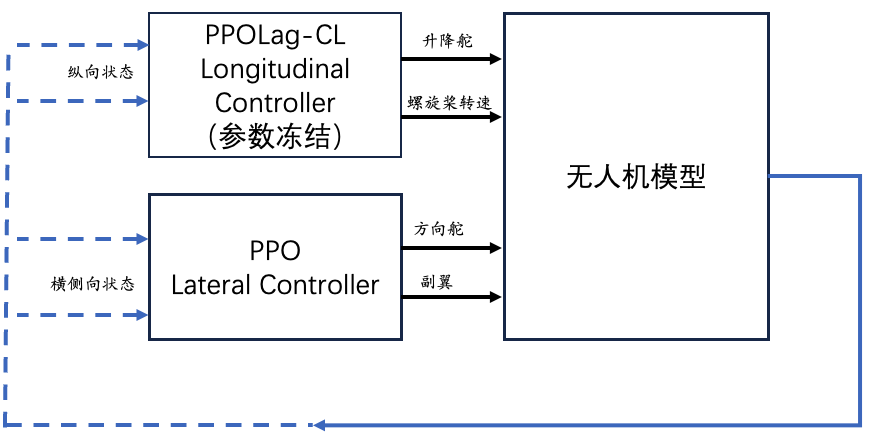
\includegraphics[width=0.8\textwidth]{chapter3/6dof.png}
\caption{\label{fig:tecs}控制框图}
\label{fig:controlblock}
\end{figure}
其中,纵向状态包括:俯仰角、俯仰角速度、水平速度、垂向速度;横向状态包括:滚转角、滚转角速率、偏航角、偏航角速率、侧向速度。

作为横向控制器的PPO相关MDP设置如下:
\begin{equation}
\begin{aligned}
s &= \left(v,v_{y},\sin \phi , \cos \phi , \sin \psi , \cos \psi ,p, r\right)^{T} \in R^{8}, \\
a &= \left(\delta_{x},\delta_{z}\right)^{T} \in R^{2},\\
R &= -(2 \phi^{2}+2\psi^{2}+2v_{y}^{2}+0.1p^{2}+0.1*r^{2})
\end{aligned}
\end{equation}

其中,横向控制器仅使用横向状态作为输入,控制量选择副翼和方向舵。
由于过渡过程中要求横向状态始终为0,因此奖励函数定义为各横向状态的平方和。训练过程如\autoref{fig:long}所示:
\begin{figure}[htb]
    \centering
    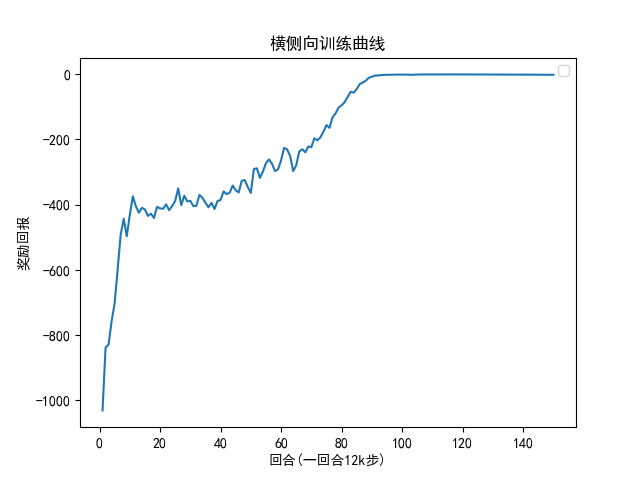
\includegraphics[width=0.6\textwidth]{chapter3/longitudal.png}
    \caption{\label{fig:tecs}横侧向训练曲线}
    \label{fig:long}
\end{figure}

可以观察到,横向控制的训练复杂性相对较低,仅需不到100次交互便可达到收敛状态。
随后,我们将初始侧向速度设定为$V_{y}=1 \ m/s$,$\phi=5^{\circ}$,$\psi=5^{\circ}$进行横向控制的仿真。
下图展示了控制效果的示意图:
\begin{figure}[H]
    \centering
    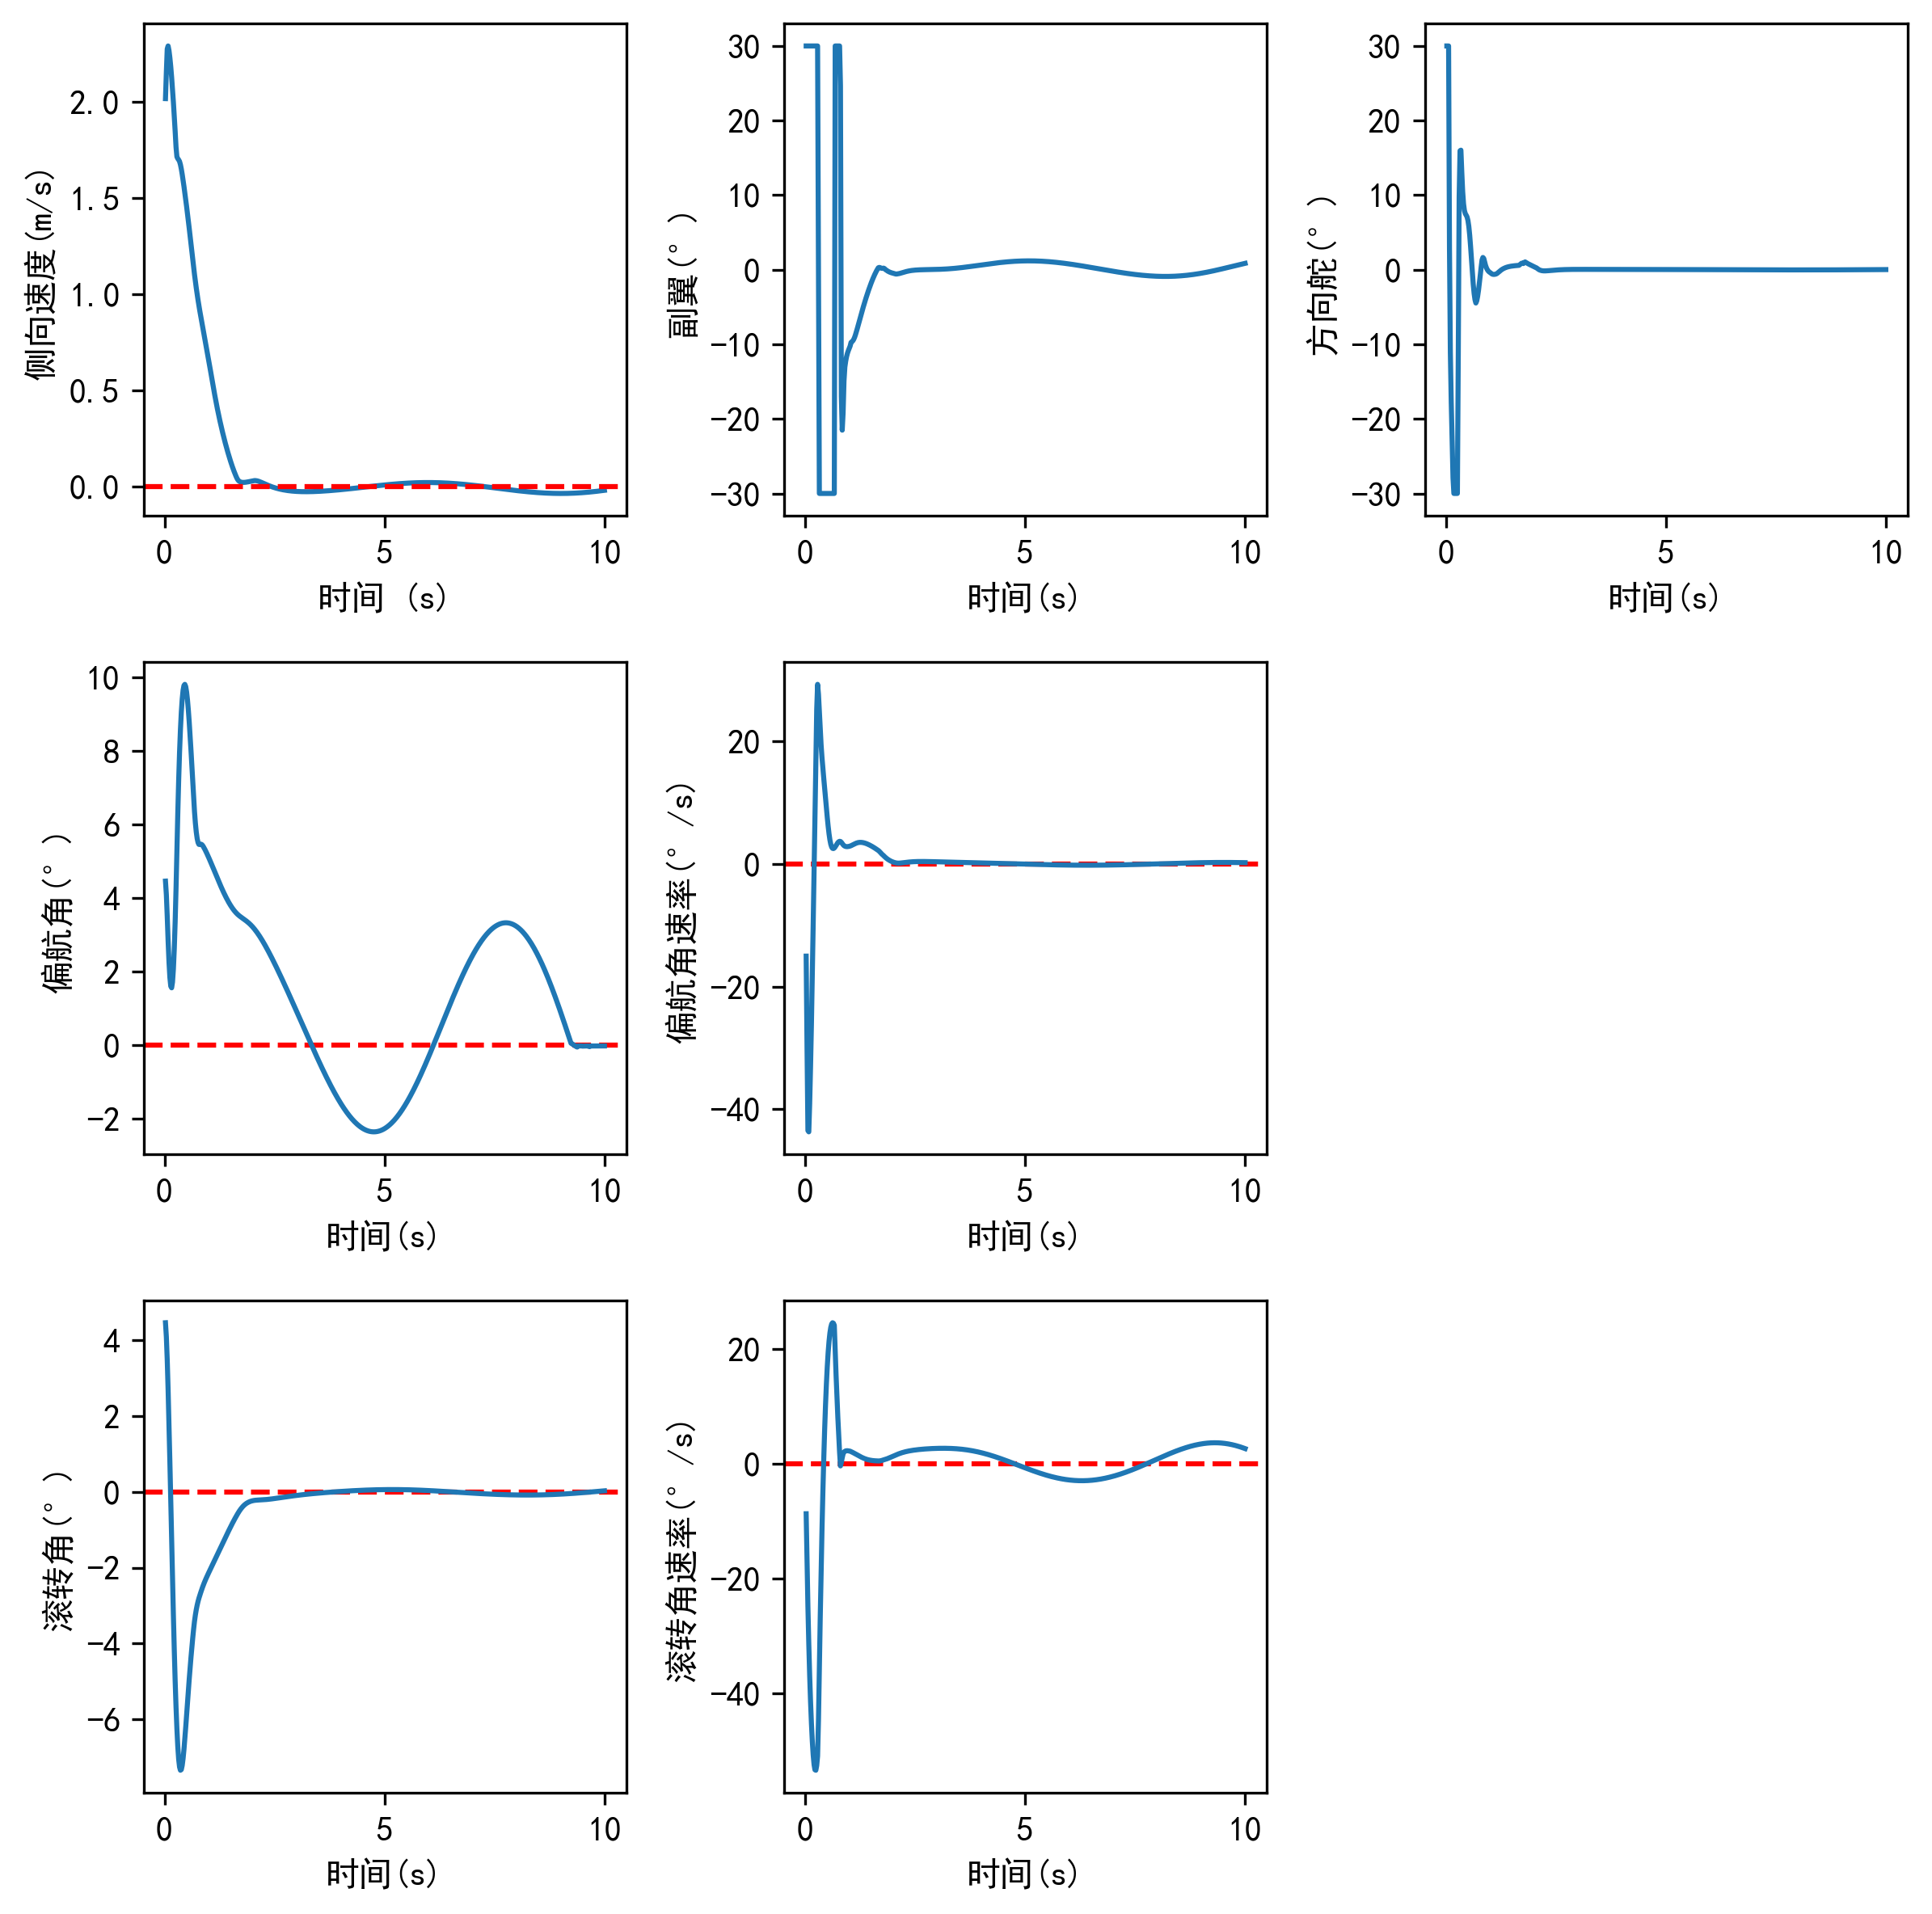
\includegraphics[width=0.9\textwidth]{chapter3/long.png}
    \caption{\label{fig:tecs}无人机横侧向控制效果}
    \label{fig:state}
\end{figure}

可以看出,横侧向控制器面对初始扰动,可以快速的恢复至零,并保持稳定,并不会受执行逆过渡过渡的纵向动力学影响。

设定初始俯仰角$11^{\circ},v_{y}=0.5m/s,\phi=5^{\circ},\psi=-5^{\circ}$,进行六自由度仿真仿真实验:
\begin{figure}[htb]
    \centering
    \includegraphics[width=0.8\textwidth]{chapter3/6dofstate.png}
    \caption{\label{fig:tecs}无人机控制量}
    \label{fig:action}
\end{figure}
如\autoref{fig:state}所示,当初始横侧向状态误差较小时,纵向过渡控制策略能够在无需微调的情况下直接迁移,实现快速定高过渡。同时,横纵向PPO控制器只需要大约100轮训练即可将横侧向误差收敛至零。
这也表明了在研究无人机过渡问题时,通常可以将无人机进行解耦,并根据无人机纵向动力学特性设计相应的过渡转换方法。观察到,快速定高过渡的优化目标是最小化过渡时间,因此为了更快地使俯仰角和速度接近
指定误差范围,控制器经常会趋于饱和状态,产生高频控制,这也对无人机的执行器带来了潜在的危害。

\section{本章总结}
本章针对涵道无人机快速定高过渡转换问题展开研究。首先,将无人机进行横纵向解耦,并以涵道无人机纵向三自由度模型为基础,将无人机快速定高过渡问题转化为带有速度约束和终端约束的时间最短问题。
针对强化学习中奖励函数调整困难的问题,提出了PPOLag算法的基本训练方案,并给出了状态空间、动作空间以及奖励函数等强化学习基础元素,
接着进行了仿真实验,说明了与常规强化学习算法相比,拉格朗日乘子的引入可以帮助智能体更好地权衡惩罚与奖励,以实现零约束违反。
并对比了非线性规划求解器GPOPS-II和总能量过渡控制算法,说明了PPOLag算法可以以较短的时间和高度变化完成快速定高过渡,同时,进行了蒙特卡洛仿真实验,验证了算法的泛化性能。
最后,将纵向控制器网络参数固定并结合PPO算法对无人横侧向控制器进行训练,并进行无人机六自由度仿真试验,表明无人机横纵向解耦的可行性。

\chapter{考虑不确定性干扰和执行器约束的逆过渡方法改进}
\section{引言}
强化学习常因泛化能力的缺失而导致算法在真实世界中的表现不佳。
特别是在确定性的马尔可夫决策过程(MDP)环境中,模型易于“过拟合”训练数据,进而在未见过的环境上性能显著降低。面对此潜在挑战,设计无人机逆过渡策略时,
应综合考量其在过渡过程中的泛化性和鲁棒性。这是为了确保无人机在遭遇模型不匹配及外部扰动时,仍能可靠完成过渡任务。
进一步地,在快速定高逆过渡任务中,尽管PPOLag算法缩短了过渡时间和降低了高度变化,但它亦带来了潜在的安全风险。
例如,在逆过渡任务的研究中,PPOLag算法所采取的控制策略展现出“Bang-Bang”式的控制特征,即控制信号在两个极端值之间急剧切换。然而,由于现实世界中执行器的速率限制,此类控制策略的实际应用可能遭遇难题,甚至有可能对执行器造成损伤。
因此,本章针对涵道无人机在面对内部参数变化、外部干扰以及执行器约束的挑战,
提出了相应的强化学习改进方法,并通过无人机的仿真性能验证,表明了所提方法的有效性。
\section{考虑不确定性干扰的策略改进方法}
\subsection{模型参数失配与外部干扰建模}
通常,在四足机器人等领域,扰动主要来自于机器人的质量、摩擦系数等自身物理参数。但由于涵道垂直起降固定翼无人机动力学的特殊性,
不仅需要考虑无人机内部参数不确定性,更需要考虑环境中潜在的风扰对无人机过渡性能带来的影响。下面将对环境中的风场进行数学建模并
给出无人机内部参数扰动分布。
\subsubsection{风场建模}
自然风通常包括常值风、阵风、紊流风与风切变,其中,风切变是描述风速随海拔高度变化而发生突变的现象,
由于快速定高过渡中高度几乎不发生变化,因此针对无人机纵向三自由度模型,
建立以$X_{e}$轴水平风为主的风场模型,并忽略风切变:
\begin{itemize}
    \item [1.] 常值风
    在常值风中,我们使用基本风速来定义风力作用过程中的基准强度。所有其他风速特性均在此基准强度之上进行衡量与叠加。基本风速旨在反映过程中风力的
    初始强度水平,其选取值紧密贴近风速的平均值。这一基本风速具有明显的稳定属性,其稳定性通过常数$k$来量化表示。
    \begin{align}
        V_{b} = k
    \end{align}
    \item [2.] 阵风模型
    阵风通常用来描述短时间内的风速变化,重点体现了风场的突发性。本文采用三角函数来描述阵风风场:
    \begin{align}
        V_{g} & = \left\{\begin{array}{l}
        0,\left(t<t_{1} \text { 或 } t>t_{1}+T_{g}\right) \\
        \frac{V_{\text {gmax }}}{2}\left(1-\cos \left(2 \pi \frac{t-t_{1}}{T_{g}}\right)\right),\left(t_{1} \leq t \leq t_{1}+T_{g}\right)
        \end{array}\right.
    \end{align}
    其中。阵风幅值$V_{\text {gmax }}=1m/s$,阵风周期$T_{g}$取1s。
    \item [3.] 紊流风
    紊流风则选取德莱顿模型(Dryden Model)\cite{abichandani2020wind},经过拉普拉斯变换后的模型传递函数为:
    \begin{align}
        H_{u}(s) & = \sigma_{u} \sqrt{\frac{2 L_{u}}{\pi V}} \cdot \frac{1}{1+\frac{L_{u}}{V} s}\\
        H_{w}(s) & = \sigma_{w} \sqrt{\frac{L_{w}}{\pi V}} \cdot \frac{1+\frac{\sqrt{3} L_{w}}{V} s}{\left(1+\frac{L_{w}}{V} s\right)^{2}}
    \end{align}
    其中,$V$表示无人机空速,$L_{u},L_{w}$表示该方向上的紊流尺度,$\sigma_{u},\sigma_{w}$表示该方向上的紊流强度,同时由于涵道无人机过渡阶段通常发生在低空阶段,
    因此,其紊流尺度与强度均以军用规范MIL-F-8785C为参照,公式如下:
    \begin{align}
        L_{w} & = h \\
        L_{l l} & = L_{v} = \frac{h}{(0.177+0.000823 h)^{1.2}}\\
        \sigma_{w} & = 0.1 W_{20} \\
        \frac{\sigma_{u}}{\sigma_{w}} &= \frac{\sigma_{v}}{\sigma_{w}} = \frac{1}{(0.177+0.000823 h)^{0.4}}
    \end{align}
\end{itemize}
其中,紊流风$u_{wg}$,$w_{wg}$由高斯白噪声经Dryden传递函数产生。综上,环境中风扰可由上述三种风场叠加产生,在机体轴下风速表示为:
\begin{equation}
    V_{w}^{b}=\begin{bmatrix}
        u_{wind}\\
    w_{wind}
    \end{bmatrix}=  \begin{bmatrix}
        (v_{b}+v_{g})\cos\theta \\
        (v_{b}+v_{g})\sin\theta
    \end{bmatrix}+\begin{bmatrix}
        u_{wg}\\
    w_{wg}
    \end{bmatrix}
\end{equation}

\subsubsection{无人机内部参数扰动}
除了外部输入的风干扰,无人机还需要解决内部参数的不确定性,例如:足够精准的气动力模型通常难以获得,因此,过渡策略还需对气动参数表现出一定的鲁棒性;
由于传感器和执行器的潜在误差,无人机还必须能够承受一定的传感器测量误差以及信号时滞,为此,结合之前风扰参数,给出无人机所面对的主要扰动参数:
\begin{table}
    \centering
    \caption{模型参数扰动}
    \label{tab:paramdisturbance}
    \begin{tabular*}{0.8\textwidth}{@{\extracolsep{\fill}}lll}
        \toprule
        扰动类型 & 噪声分布 & 参数变化范围 \\
        \midrule
        质量扰动\( \left [ kg \right ]  \) & 均匀分布 &  \( \le 5\% \)\\
        转动惯量扰动\( \left [ kg \cdot m^{2} \right ]  \) & 均匀分布 & \( \le 5\% \) \\
        升力系数\(C_{L}\) & 均匀分布 & \( \le 20\% \) \\
        阻力系数\(C_{D}\) & 均匀分布 & \( \le 20\% \) \\
        俯仰力矩系数\(C_{m} \) & 均匀分布 & \( \le 20\% \) \\
        传感器信号时滞\( \left [ s \right ]  \) & 指数分布 & \(\lambda\in  \text{Uniform}[ 250,1000] \) \\
        俯仰角传感器误差\( \left [ rad \right ]  \) & 高斯分布 & \(\mu = 0.0 ,\sigma = 6.325 \cdot 10^{-4}\) \\
        角速率传感器误差\( \left [ rad/s \right ]  \) & 高斯分布 & \( \mu = 0.0 ,\sigma = 6.325 \cdot 10^{-4}\) \\
        速度传感器误差\( \left [ m/s \right ]  \) & 高斯分布 & \( \mu = 0.0 ,\sigma = 0.029 \) \\
        常值风扰动\( \left [ m/s \right ]  \) & 均匀分布 & [-4,4]  \\
        阵风扰动开始时间\( \left [ s \right ]\) &均匀分布 & [0,10]\\
        \bottomrule
    \end{tabular*}
\end{table}

其中,传感器信号时滞描述了在实际飞行中,传感器信号接受的时间间隔并非固定的(本文为0.02s),而是服从指数分布\cite{bohn2023data}。
传感器误差分布则是参考Cessna Citation飞行器\cite{lee2021online}。

\subsubsection{训练环境设置}
为了提供更好地鲁棒性与泛化性能,我们使用领域随机化技术在训练时根据\autoref{paramdisturbance}进行采样从而对环境参数进行随机化,此时优化目标为:
\begin{align}
    &\max _{\pi \in \Pi_{\theta}} \underset{m \sim p_{\phi}}{\mathbb{E}}\left [J_{R}(\pi)   \right ] 
\end{align}
其中,$p_{\phi}$是环境参数的分布。

同时,为了更好地优化环境参数分布下的智能体性能,在训练环境中引入并行Actor-Critic架构(synchronized parallel actor-critic)提高数据采样效率,流程如\autoref{fig:parallel}所示。
\begin{figure}[htbp]
    \centering
    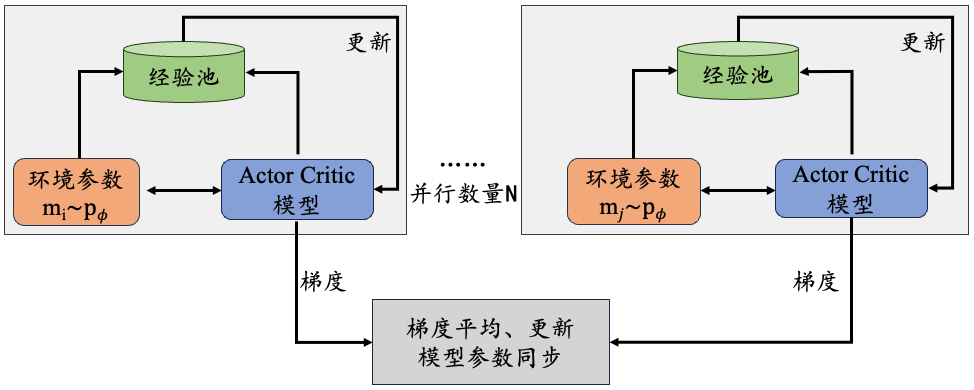
\includegraphics[width=0.75\textwidth]{chapter4/parallel.png}
    \caption{\label{fig:parallel}并行训练架构}
    \label{fig:action}
\end{figure}

综上,我们对无人机在逆过渡过程中的干扰进行建模,并利用领域随机化及同步并行训练架构对训练环境进行了优化。
\subsection{基于值函数约束的近端策略优化算法改进}
\subsubsection{VCPPOLag算法原理}
在处理约束问题时,采用拉格朗日松弛技术的PPOLag算法展现出了一定的局限性:其无法有效降低约束成本,导致成本在给定的阈值附近振荡。具体来说,如
RCPO\cite{tessler2018reward}、CPO\cite{achiam2017constrained}和PPOLag算法训练效果所示,成本阈值的降低并非持续性,
而是可能经历初期下降后又回升至接近成本阈值的水平。这一现象源于拉格朗日乘子在约束成本低于成本阈值时的迅速归零,从而阻碍了系统向降低约束成本的方向进一步更新。
\begin{figure}[htbp]
    \centering
    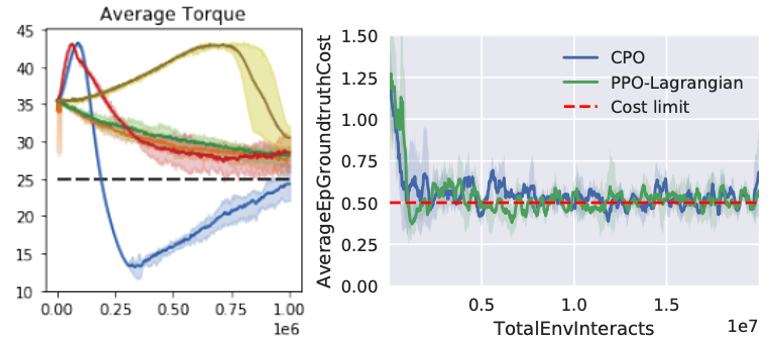
\includegraphics[width=0.75\textwidth]{chapter4/otheralgo.png}
    \caption{\label{fig:otheralgo}RCPO(左)与PPOLag,CPO(右)算法}
\end{figure}

在\autoref{chapter:env}的成本函数设置中,我们将成本阈值$d$设为零,因此未遇到成本阈值无法降低的问题。

而当环境参数遭遇扰动,始终为零的成本阈值就无法适用:例如,在顺风条件下,无人机的空速
相对减少,进而导致空气阻力降低。而在整个定高过渡过程中,能量的主要消耗来源于空气阻力的作用。因此,为了在顺风条件下达到类似于无风状态的过渡时间,
无人机需通过违反约束来调整飞行高度来消耗额外能量。从理论上讲,若存在N个环境实例,那么d值应该取N个环境对应的最小成本阈值的最大值。

然而,这种方法在实际操作中面临挑战:通常需要多次实验才能确定适当的成本阈值。成本阈值过低可能使智能体过于保守,
限制其探索能力;而成本阈值过高则可能导致约束成本先降后升,影响智能体满足约束的性能。

而在最优控制理论中,无人机的最终状态是否达到特定范围通常不是主要关注点,因为最优控制会将最终状态视为约束条件之一。

借鉴\parencite{bohez2019value}中为处理能量最优化问题而对动作值函数加以限制的思想,我们提出了
VCPPOLag(Value Constrained PPOLag)算法来对干扰下的过渡任务进行训练。此方法通过交换优化目标与约束的优化顺序,确保在完成任务的前提下减少约束违反的次数。
算法原理如下:

在\autoref{chapter:env},我们给出了一种类似稀疏奖励的奖励函数设置,当无人机成功完成过渡时将会获得一个较大的终端奖励$\kappa$,
无人机状态值函数定义为:
\begin{align}
    V^{\pi}\left(s\right) = \mathbb{E}_{\pi }\left[\sum_{k = 0}^{\infty} \gamma^{k} R_{t+k+1}\mid S_{t}= s\right]
\end{align}
其中,当策略固定时,初始状态下的价值函数表达为:
\begin{align}
    V_{\pi}\left(s_{0}\right) = \sum_{t = 0}^{T} \gamma^{t} R_{t+1}
\end{align}
设能够完成过渡任务的智能体的策略为$\pi_{success}$,根据本文奖励函数的设置,对于所有能够完成任务的策略有初始状态价值函数定义如下:
\begin{align}
    V_{\pi_{success}}\left(s_{0}\right) \approx   \gamma^{T} \cdot \kappa
\end{align}
其中,$T$表示期望过渡时间,在本文中设$\bar{T}$为无风状态下的平均过渡时间。
因此,强化学习的优化目标变为
\begin{align}
    &\min _{\pi \in \Pi_{\theta}} J_{C}(\pi) \\
    &\text { s.t. } J_{R}(\pi)=V_{\pi}(s_{0}) \ge \gamma^{\bar{T}}\kappa
\end{align}
归一化后的优势值函数定义如下:
\begin{align} 
    {A}_{\lambda^{\prime}}^{\pi_{k}}(s, a)&=\frac{-\lambda A_{R}^{\pi_{k}}(s, a) +  A_{C_{i}}^{\pi_{k}}(s, a)}{1+ \lambda} 
\end{align}
内部的最大化问题此时变为:
\begin{align}
    \underset{\lambda}{\operatorname{maxmize}} \ \underset{\tau \sim \pi_{k}}{\mathbb{E}}\left[\lambda_{i}\left[(\gamma^{\bar{T}}\kappa-V_{\pi_{k}}(s_{0}))+r(\theta)A_{R}^{\pi_{k}}(s, a)\right]\right]
\end{align}
在$ \underset{\tau \sim \pi_{k}}{\mathbb{E}}\left[A_{R}^{\pi_{k}}(s, a)\right]= 0$的假设下,拉格朗日乘子$\lambda$更新方程如下:
\begin{align}
    \lambda_{i} \leftarrow \underset{\lambda_{i}}{\operatorname{proj}}\left[\lambda_{i}-\alpha\left(V_{\pi_{k}}(s_{0})-\gamma^{\bar{T}}\kappa\right)\right]
\end{align}

综合所述,本文阐述了VCPPOLag算法的关键步骤,其主要改进在于利用稀疏奖励机制,将初始价值函数的约束视为对无人机终端状态的间接约束。因此,通过设定初始价值函数的下限,结合期望的平均过渡时间和折扣因子,
可以计算出初始状态值函数的下届。因此一旦智能体满足给定的初始状态值函数约束,它便会更新其策略,以降低约束成本,确保约束成本的最小化,有效规避了PPOLag等常规约束强化学习方法中可能遇到的约束成本反弹现象。

\subsection{基于鲁棒对抗的逆过渡方法改进}
尽管结合领域随机化的VCPPOLag算法,能在一定程度上提升智能体的鲁棒性与泛化能力,但存在以下两个不足:
1、在实践中,由于时间和资源的限制,不可能对所有潜在的环境扰动进行充分采样,导致总有部分训练分布未能覆盖。
2、领域随机化的目的是最大化期望环境参数分布下的性能,而并非最’坏‘环境条件下的性能表现,这可能导致智能体的鲁棒性不足,从而缺乏对未知分布的泛化能力。

鉴于上述不足,为了增强智能体的鲁棒性和对未曾遭遇测试分布的泛化能力,本文采用RARL\cite{pinto2017robust}中提出的鲁棒对抗攻击框架对策略进行改进。具体来说,
是通过训练一个对手模型主动选择环境扰动,而不是依赖随机抽样,实施这种方法。该框架借鉴了二人零和博弈的理论,目的是在存在潜在“对手”的情况下,训练智能体学习如何最大化其期望的累积回报。
其算法原理介绍如下:

鲁棒对抗框架可被构建为一个涉及双方参与的零和马尔科夫决策博弈,在该框架下马尔科夫决策过程可以被表达为$\left(\mathcal{S}, \mathcal{A}_{1}, \mathcal{A}_{2}, \mathcal{P}, r, \gamma\right)$,
其中,$\mathcal{A}_{1}$表示为我方智能体的动作空间,$\mathcal{A}_{2}$表示为对手的动作空间。
$\mathcal{P}: \mathcal{S} \times \mathcal{A}_{1} \times \mathcal{A}_{2} \times \mathcal{S} \rightarrow \mathbb{R}$定义为在对手行动空间影响下的状态转移概率函数,
而$r: \mathcal{S} \times \mathcal{A}_{1} \times \mathcal{A}_{2} \rightarrow \mathbb{R}$则描述了在双方行动共同影响下的奖励函数。
其中,我方智能体旨在最大化策略$\mu$下的累计折扣奖励,而对手目的则是最小化其策略$\nu$下的累计折扣奖励。

具体而言,双方的行动空间及奖励函数定义如下::
\begin{align}
    \mathcal{A}_{1} & = \left ( \omega_{p},\delta_{y} \right ) \\
    \mathcal{A}_{2} & = \left (V_{w_{x}}, V_{w_{z}}\right )\\
    r_{2}(&s,a,s^{\prime})=-r_{1}(s,a,s^{\prime})
\end{align}
我们将对手的动作设定为环境的风速,这是因为对于逆过渡过程而言,风扰往往是其最大的干扰并十分影响性能。

智能体的奖励函数定义为:
\begin{align}
    R^{1}=E_{s_{0} \sim \rho, a^{1} \sim \mu(s), a^{2} \sim \nu(s)}\left[\sum_{t=0}^{T-1} r^{1}\left(s, a^{1}, a^{2}\right)\right]
\end{align}
基于零和博弈的纳什均衡策略,最优奖励函数可表示为:
\begin{align}
    R^{1 *} & = \min _{\nu} \max _{\mu} R^{1}(\mu, \nu) = \max _{\mu} \min _{\nu} R^{1}(\mu, \nu)
\end{align}
鉴于连续行动空间下零和矩阵博弈求解的复杂性,本研究采用固定策略的求解方法:首先学习主体的策略,同时固定对手策略;
然后,固定主体策略,优化对手策略。通过迭代此过程直至策略收敛,实现两个玩家策略的优化。在每个迭代周期中,首先在保持对手参数不变的情况下,
优化主体参数以最大化滚动函数值,该函数根据给定的环境定义和双方策略对轨迹进行采样。随后,对主体参数固定,优化对手参数。通过重复此交替优化
过程,直至在预定的迭代次数后达到稳定,实现对零和博弈中纳什均衡策略的近似。

综上,我们结合VCPPOLag算法以及鲁棒对抗框架给出算法流程:
\begin{algorithm}[H]
    \begin{algorithmic}[1] % enter the algorithmic environment
        \STATE \textbf{初始化}:给定进程数量$n$,在每个进程下,随机初始化策略网络 $\pi_{\mu,\theta_{0}}$, 值函数网络 $V_{R}^{\mu,\phi_{0}}$,对手策略网络 $\pi_{\nu,\theta_{0}}$, 对手值函数网络 $V_{R}^{\nu,\phi_{0}}$, 成本值函数网络 $V_{C}^{\psi_{0}}$, 期望过渡步数$t$, $\forall i$迭代更新次数$N$
        \FOR{$k$ in $0,1,2, \ldots, K$}
        \STATE 固定对手策略$\pi_{\nu,\theta_{k}}$,使用策略$\pi_{\mu,\theta_{k}}$与无人机环境进行交互,运行$T$步收集轨迹$\tau$
        \STATE 根据奖励$R$,使用GAE估计优势值函数$\hat{A}_{R}^{\mu,\pi_{\theta_{k}}}\left(s_{t}, a_{t}\right)$,并计算$V_{tar}^{\mu,\phi_{k}}\left(s_{t}\right)=\hat{A}_{R}^{\mu,\pi_{\theta_{k}}}\left(s_{t}, a_{t}\right)+\hat{V}_{R}^{\mu,\pi_{k}}(s_{t})$
        \STATE 根据约束成本$C$,使用GAE估计优势值函数$\hat{A}_{C_{i}}^{\pi_{\theta_{k}}}\left(s_{t}, a_{t}\right)$,计算$V_{C,tar}^{\phi_{k}}\left(s_{t}\right)=\hat{A}_{C_{i}}^{\pi_{\theta_{k}}}\left(s_{t}, a_{t}\right)+\hat{V}_{C}^{\pi_{k}}(s_{t})$
            \FOR{$i$ in $0,1,2, \ldots, N$}
                \FOR{each minibatch}
                    \STATE \textbf{计算初始状态价值函数} ${V}_{R}^{\mu,\pi_{k}}(s_{0}),s_{0}\sim p$
                    \STATE \textbf{更新拉格朗日乘子}:$\lambda_{i}^{k+1} \leftarrow \underset{\lambda_{i}}{\operatorname{proj}}\left[\lambda_{i}^{k}+\alpha\left(\gamma^{t}-{V}_{R}^{\mu,\pi_{k}}(s_{0})\right)\right]$
                    \STATE \textbf{更新Critic网络}:$\phi_{\mu,k+1}=\arg \min _{\phi}\text{MSE}\left(V_{R}^{\mu,\phi_{k}}\left(s_{t}\right)-V_{tar}^{\mu,\phi_{k}}\left(s_{t}\right)\right)^{2}$
                    \STATE \textbf{更新CostCritic网络}:$\psi_{k+1}=\arg \min _{\psi}\text{MSE}\left(V_{C}^{\psi_{k}}\left(s_{t}\right)-V_{C,tar}^{\psi_{k}}\left(s_{t}\right)\right)^{2}$
                    \STATE \textbf{计算ActorLoss} 根据 \autoref{aloss}
                    \STATE \textbf{更新Actor网络}:$\theta \leftarrow \theta-\eta \nabla L^{C L I P}(\theta)$
                \ENDFOR
                \STATE 固定无人机过渡策略$\pi_{\mu,\theta_{k}}$,对手使用策略$\pi_{\nu,\theta_{k}}$与无人机环境进行交互,运行$T$步收集轨迹$\tau$
                \FOR{each minibatch}
                    \STATE \textbf{更新对手Critic网络}:$\phi_{\mu,k+1}=\arg \min _{\phi}\text{MSE}\left(V_{R}^{\mu,\phi_{k}}\left(s_{t}\right)-V_{tar}^{\mu,\phi_{k}}\left(s_{t}\right)\right)^{2}$
                    \STATE \textbf{计算ActorLoss} 根据 \autoref{aloss}
                    \STATE \textbf{更新对手Actor网络}:$\theta \leftarrow \theta-\eta \nabla L^{C L I P}(\theta)$
                \ENDFOR
            \ENDFOR
        \ENDFOR
        \STATE \textbf{输出}:策略网络参数$\theta$
    \end{algorithmic}
    \caption{\label{alg:ppolag}鲁棒对抗VCPPOLag算法}
\end{algorithm}
\subsection{实验仿真与结果分析}
本节采用了Intel(R) Xeon(R) Gold 5220 CPU 2.20GHz 18核心和NVIDIA GeForce 2080TI GPU进行对上述改进算法进行仿真实验,
实验首先基于领域随机化技术,将VCPPOLag算法与具备不同成本阈值的PPOLag算法进行对比,以验证VCPPOLag算法的有效性。随后,我们对
结合鲁棒攻击的VCPPOLag算法执行了鲁棒性与泛化性能测试,结果表明鲁棒攻击能够在一定程度上提升算法的泛化性能。在评估过程中,为保证
评估的公正性,我们选取了多个随机种子进行蒙特卡洛仿真,同时列出了训练过程中相关的超参数如\autoref{tab:algo1_config}。
\begin{table}[htbp]
    \centering % 居中
    \caption{\label{tab:algo1config}鲁棒对抗VCPPOLag算法超参数}
    \begin{tabularx}{0.7\linewidth}{|c|X|c|}
        \hline
        参数 & 参数说明 & 参数值 \\ \hline
        parallel num& 并行进程数量 & 10 \\ \hline
        steps per epoch & 一回合交互步数 & 12000 \\ \hline
        update iters & 一回合更新次数 & 20 \\ \hline
        batch size & 64 & 批处理容量\\ \hline
        entropy coef & 熵损失系数 & 0.01 \\ \hline
        max grad norm & 梯度裁剪阈值 & 40.0 \\ \hline
        critic norm coef & 价值函数正则项 & 0.001 \\ \hline
        gamma & 折扣因子 & 0.99 \\ \hline
        lam & 广义优势估计参数 & 0.95 \\ \hline
        clip & 裁剪比 & 0.2 \\ \hline
        std & 策略分布方差 & [0.1,0.5] \\ \hline
        feature dim & 策略/价值神经网络隐藏层 & [128,128] \\ \hline
        activation & 激活函数 & tanh \\ \hline
        learning rate & 学习率 & 0.0003 \\ \hline
        value limit & 价值函数阈值 & 40.0 \\ \hline
        lag init & 拉格朗日乘子初值 & 1.0 \\ \hline
        lag learning rate & 拉格朗日乘子学习率 & 0.035 \\ \hline
    \end{tabularx}
\end{table}

\subsubsection{VCPPOLag算法验证}
为了阐明VCPPOLag算法的优势,在环境干扰下,
以PPOLag算法为基准,通过调整不同的成本阈值进行了一系列对比实验。
特别地,为保证比较的公正性,本研究在VCPPOLag算法中采用拉格朗日乘数的逆作为实验参数,以此对比PPOLag中拉格朗日乘数的功能与影响。
训练过程如\autoref{fig:vcppolag}:
\begin{figure}[H]
    \centering
    % 第一行
    \begin{subfigure}{.5\textwidth}
        \centering
        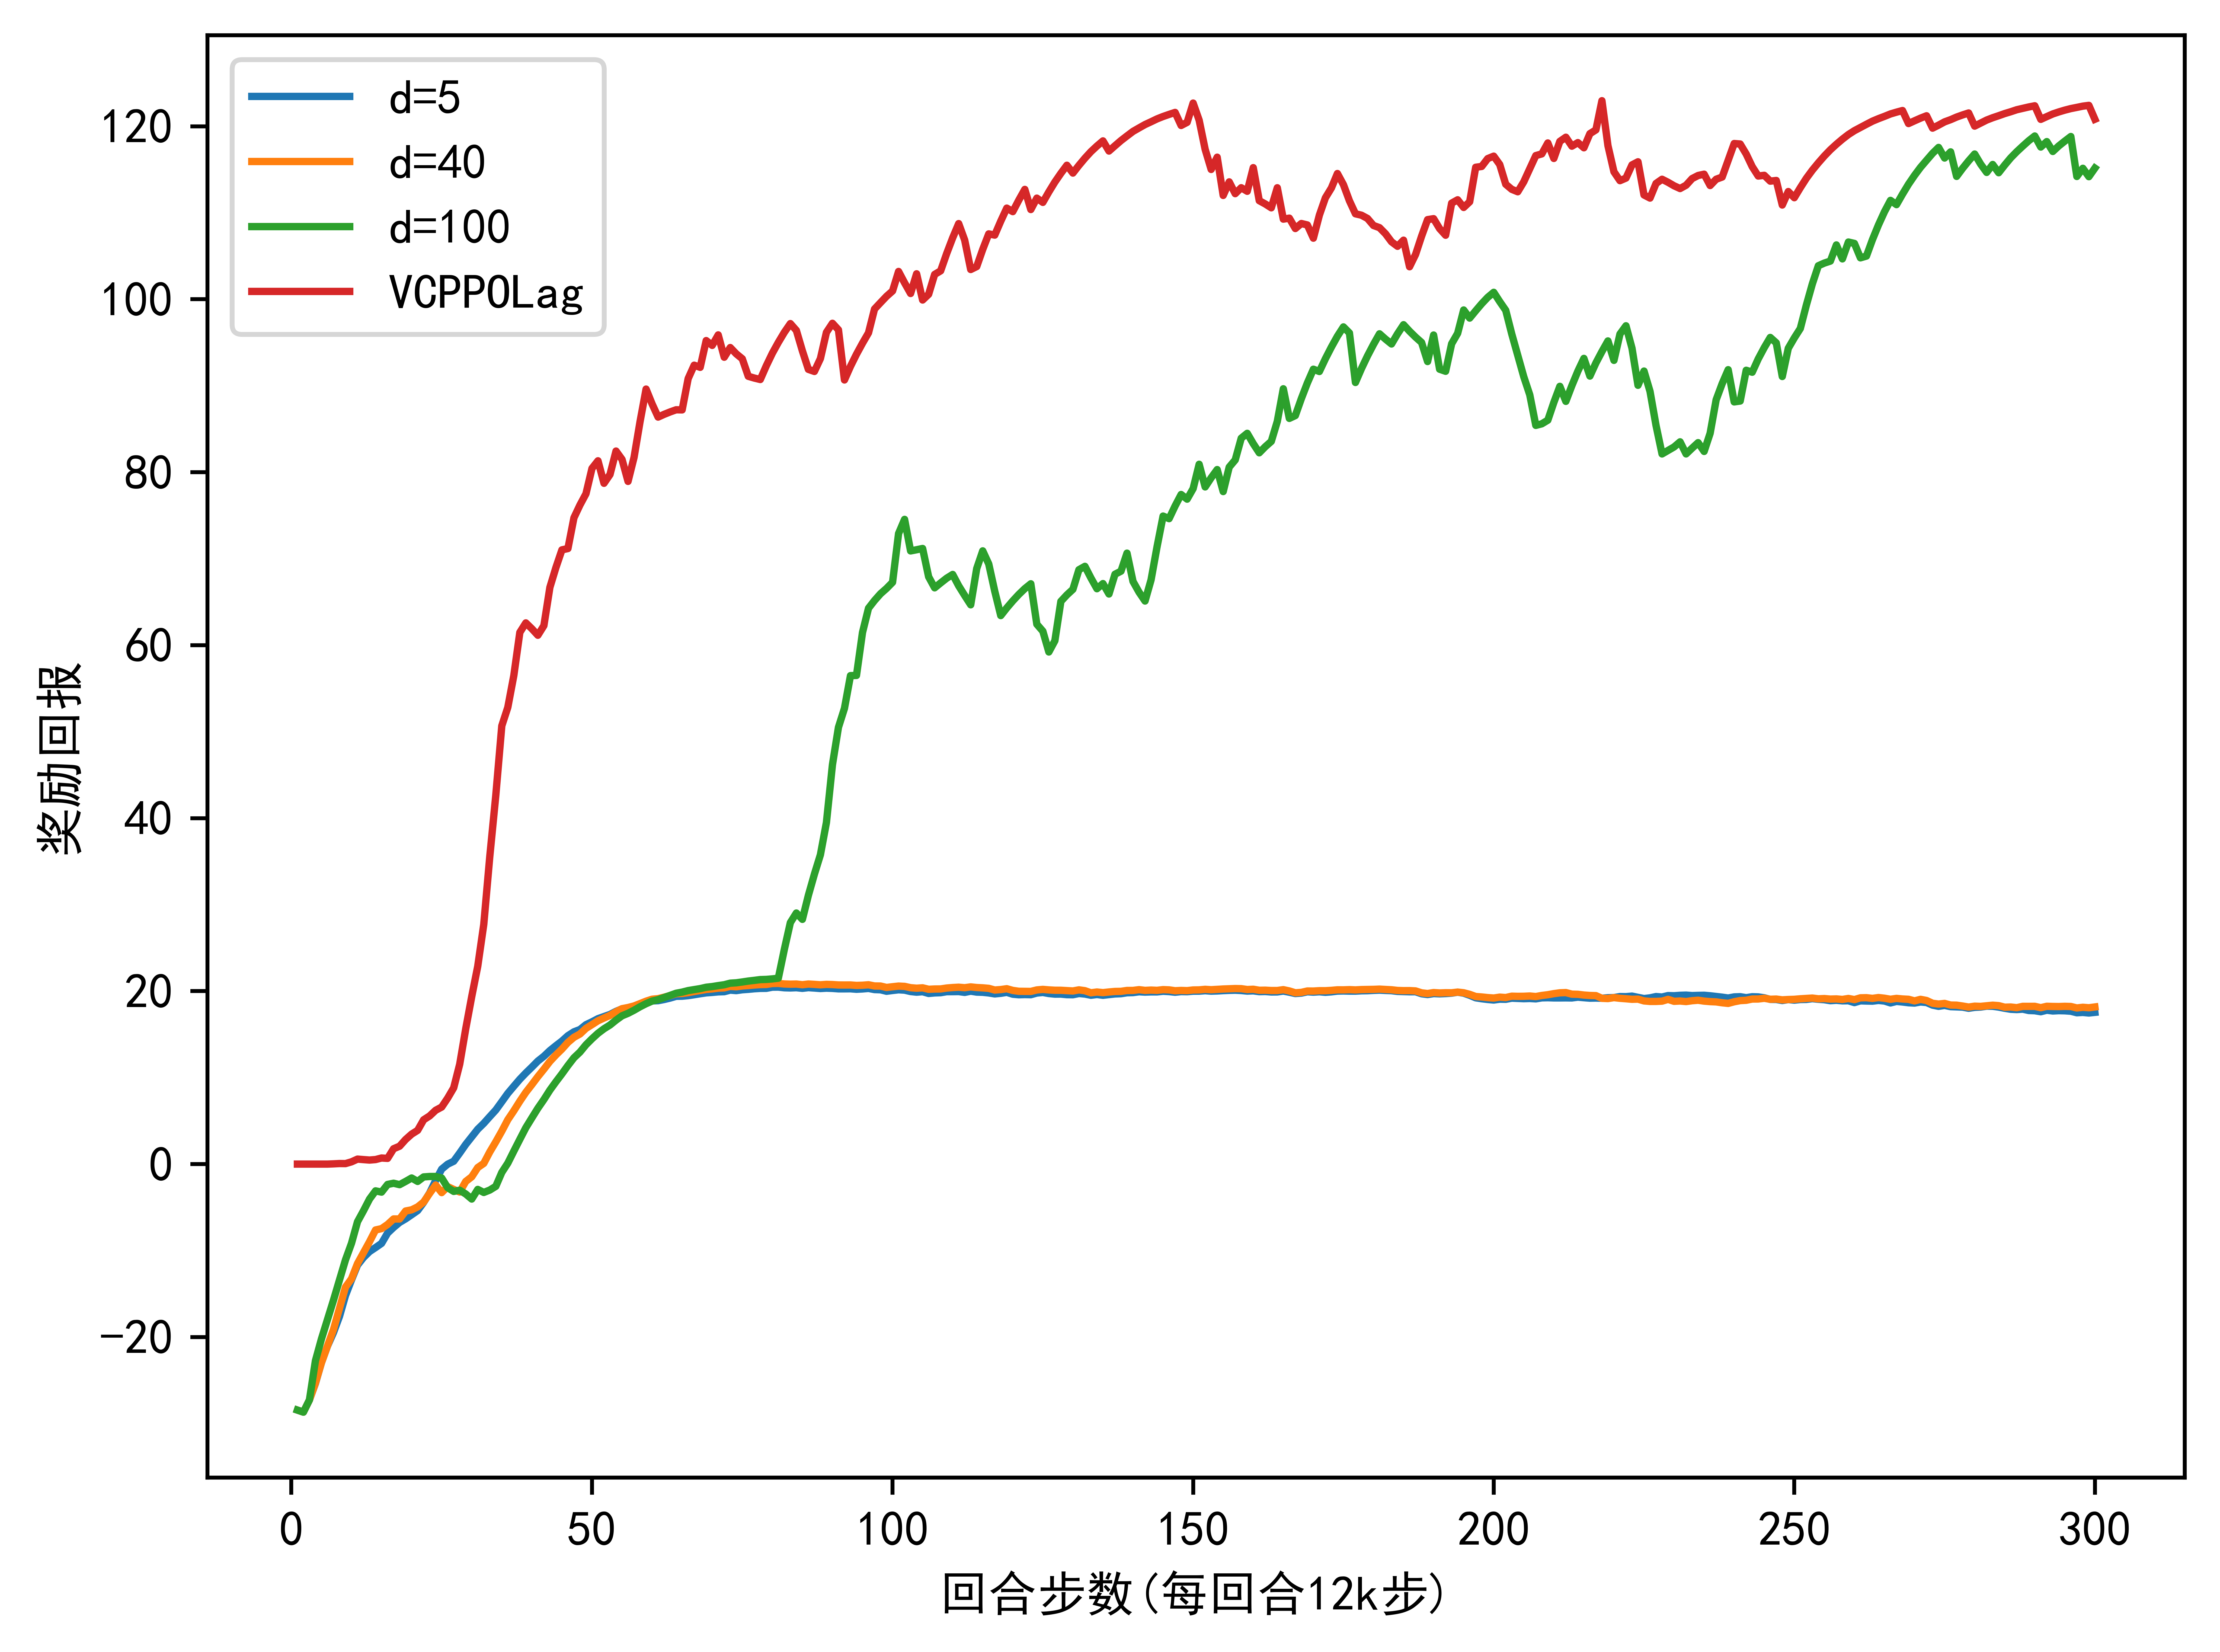
\includegraphics[width=0.9\linewidth]{chapter4/vccmpreward.png}
        \caption{Reward comparison}
        \label{fig:reward}
    \end{subfigure}%

    \begin{subfigure}{.5\textwidth}
        \centering
        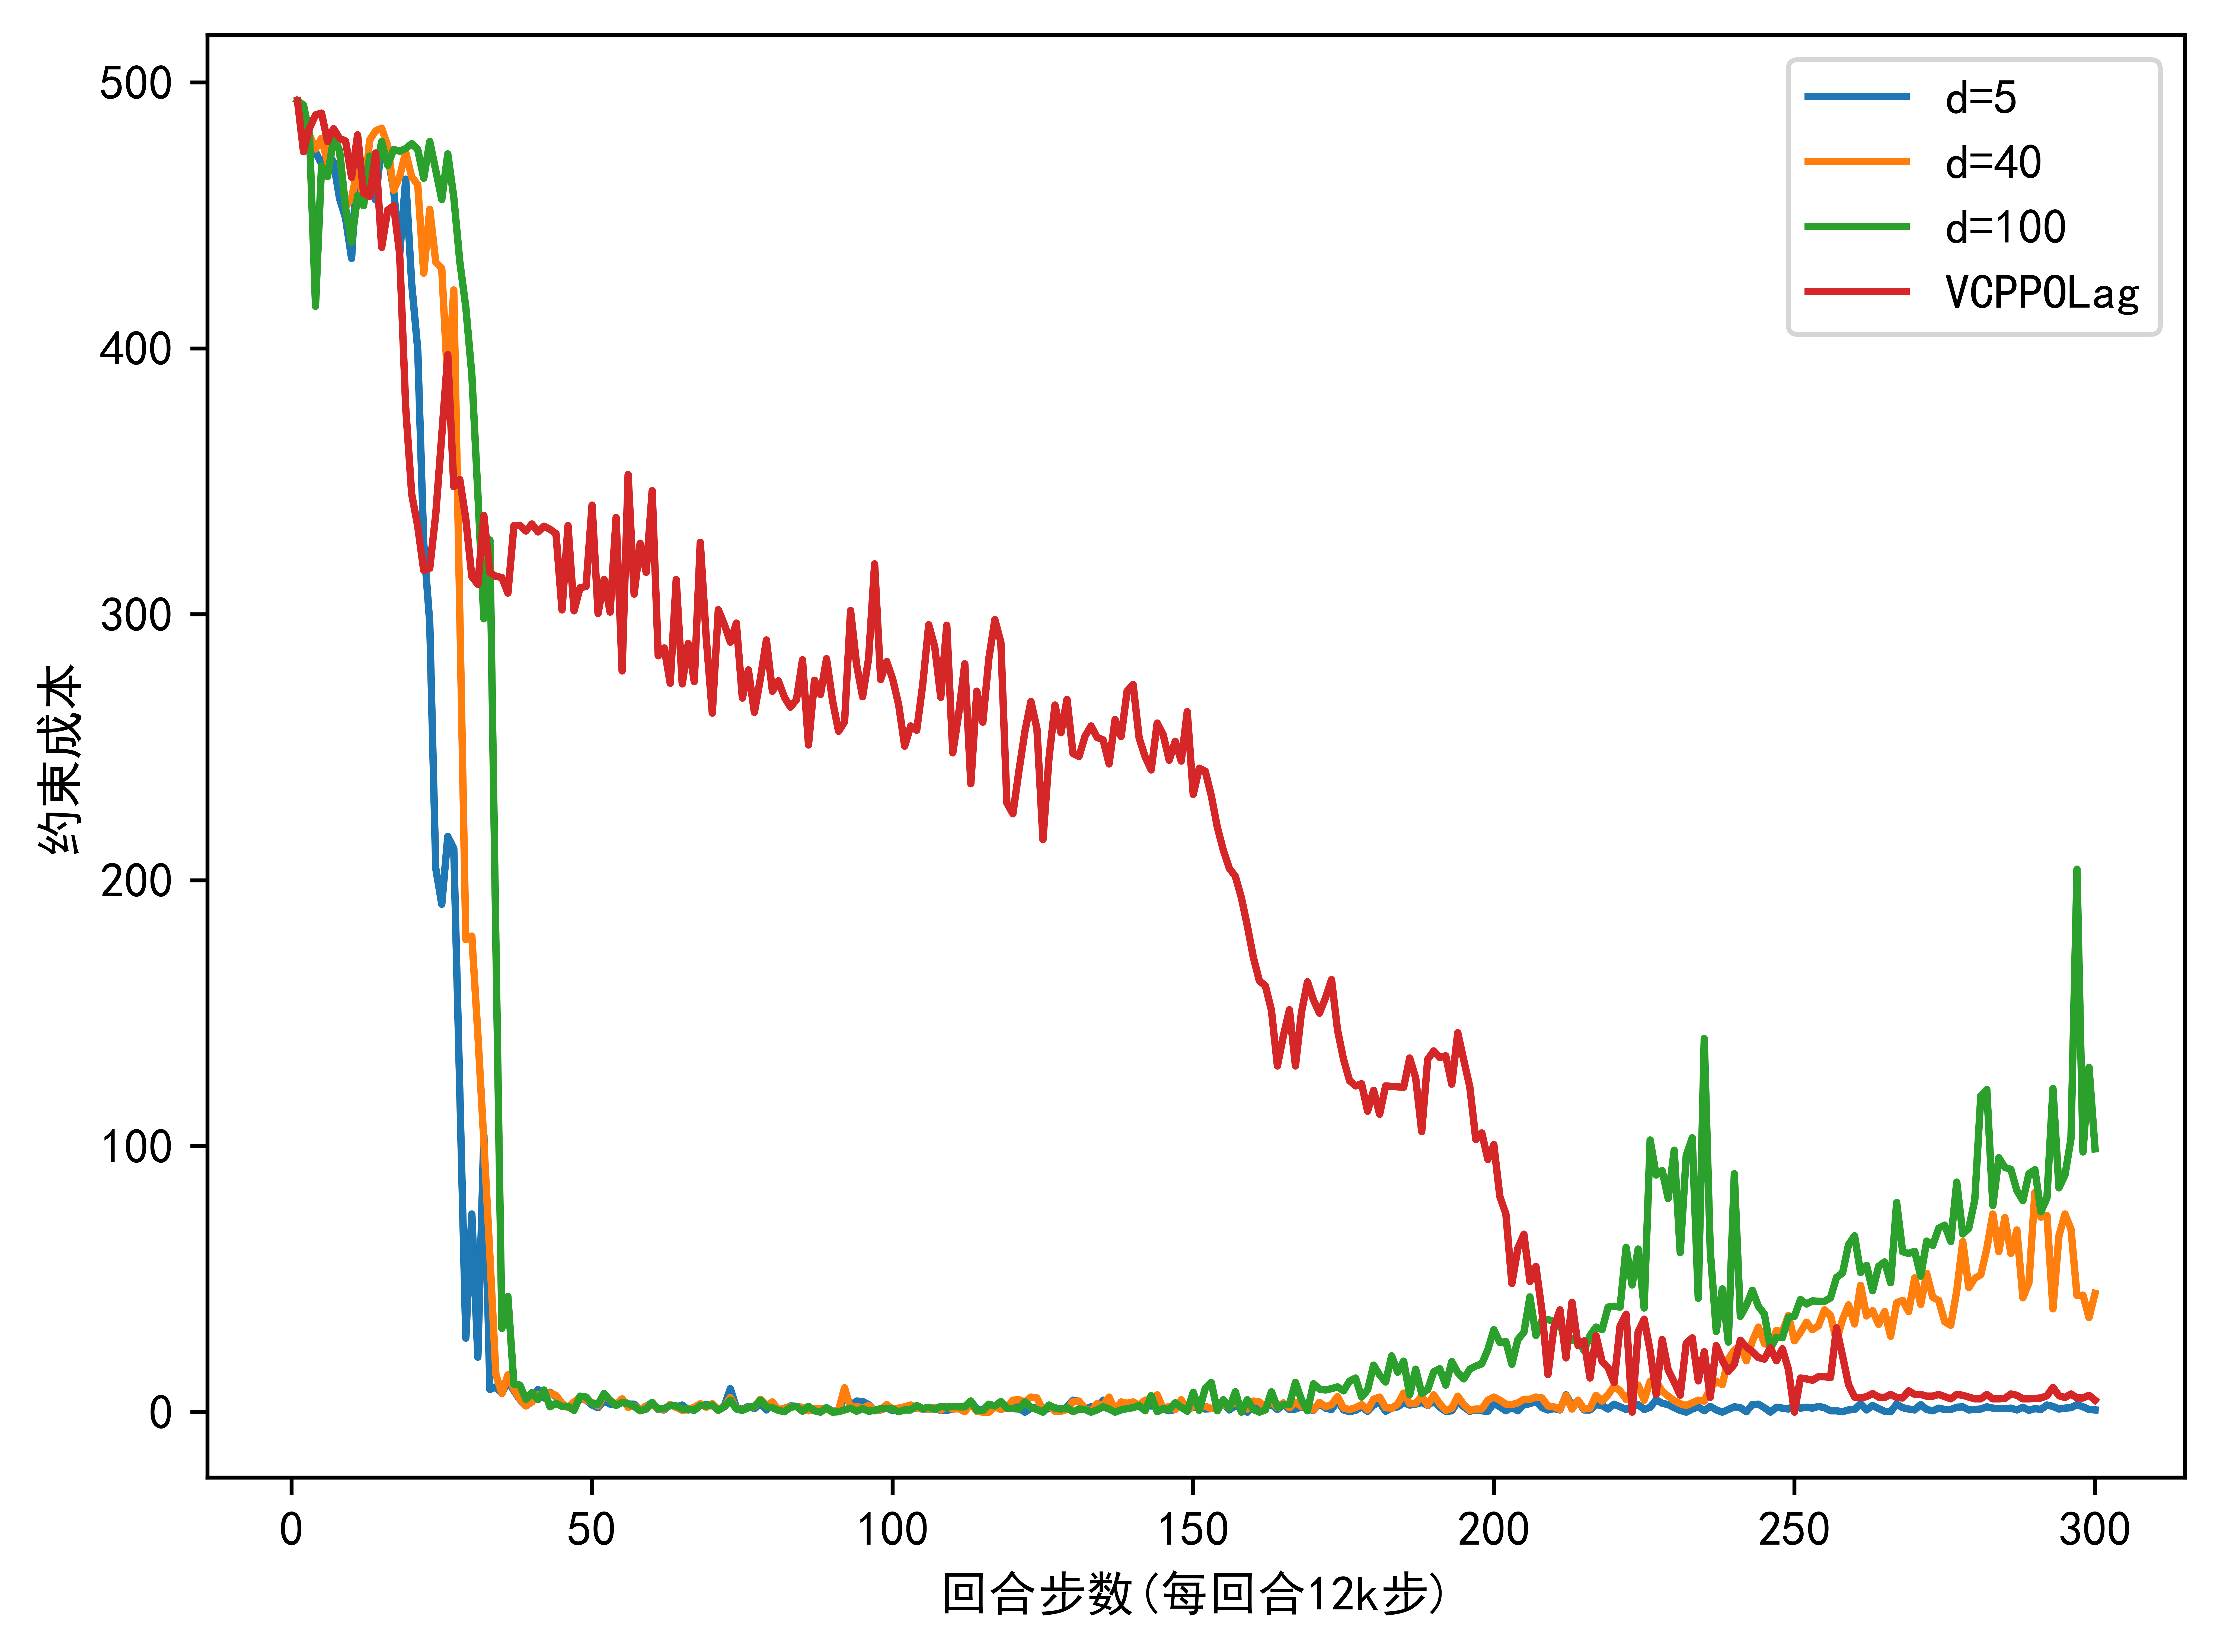
\includegraphics[width=0.9\linewidth]{chapter4/vccmpcost.png}
        \caption{Cost comparison}
        \label{fig:cost}
    \end{subfigure}

    \begin{subfigure}{.5\textwidth}
        \centering
        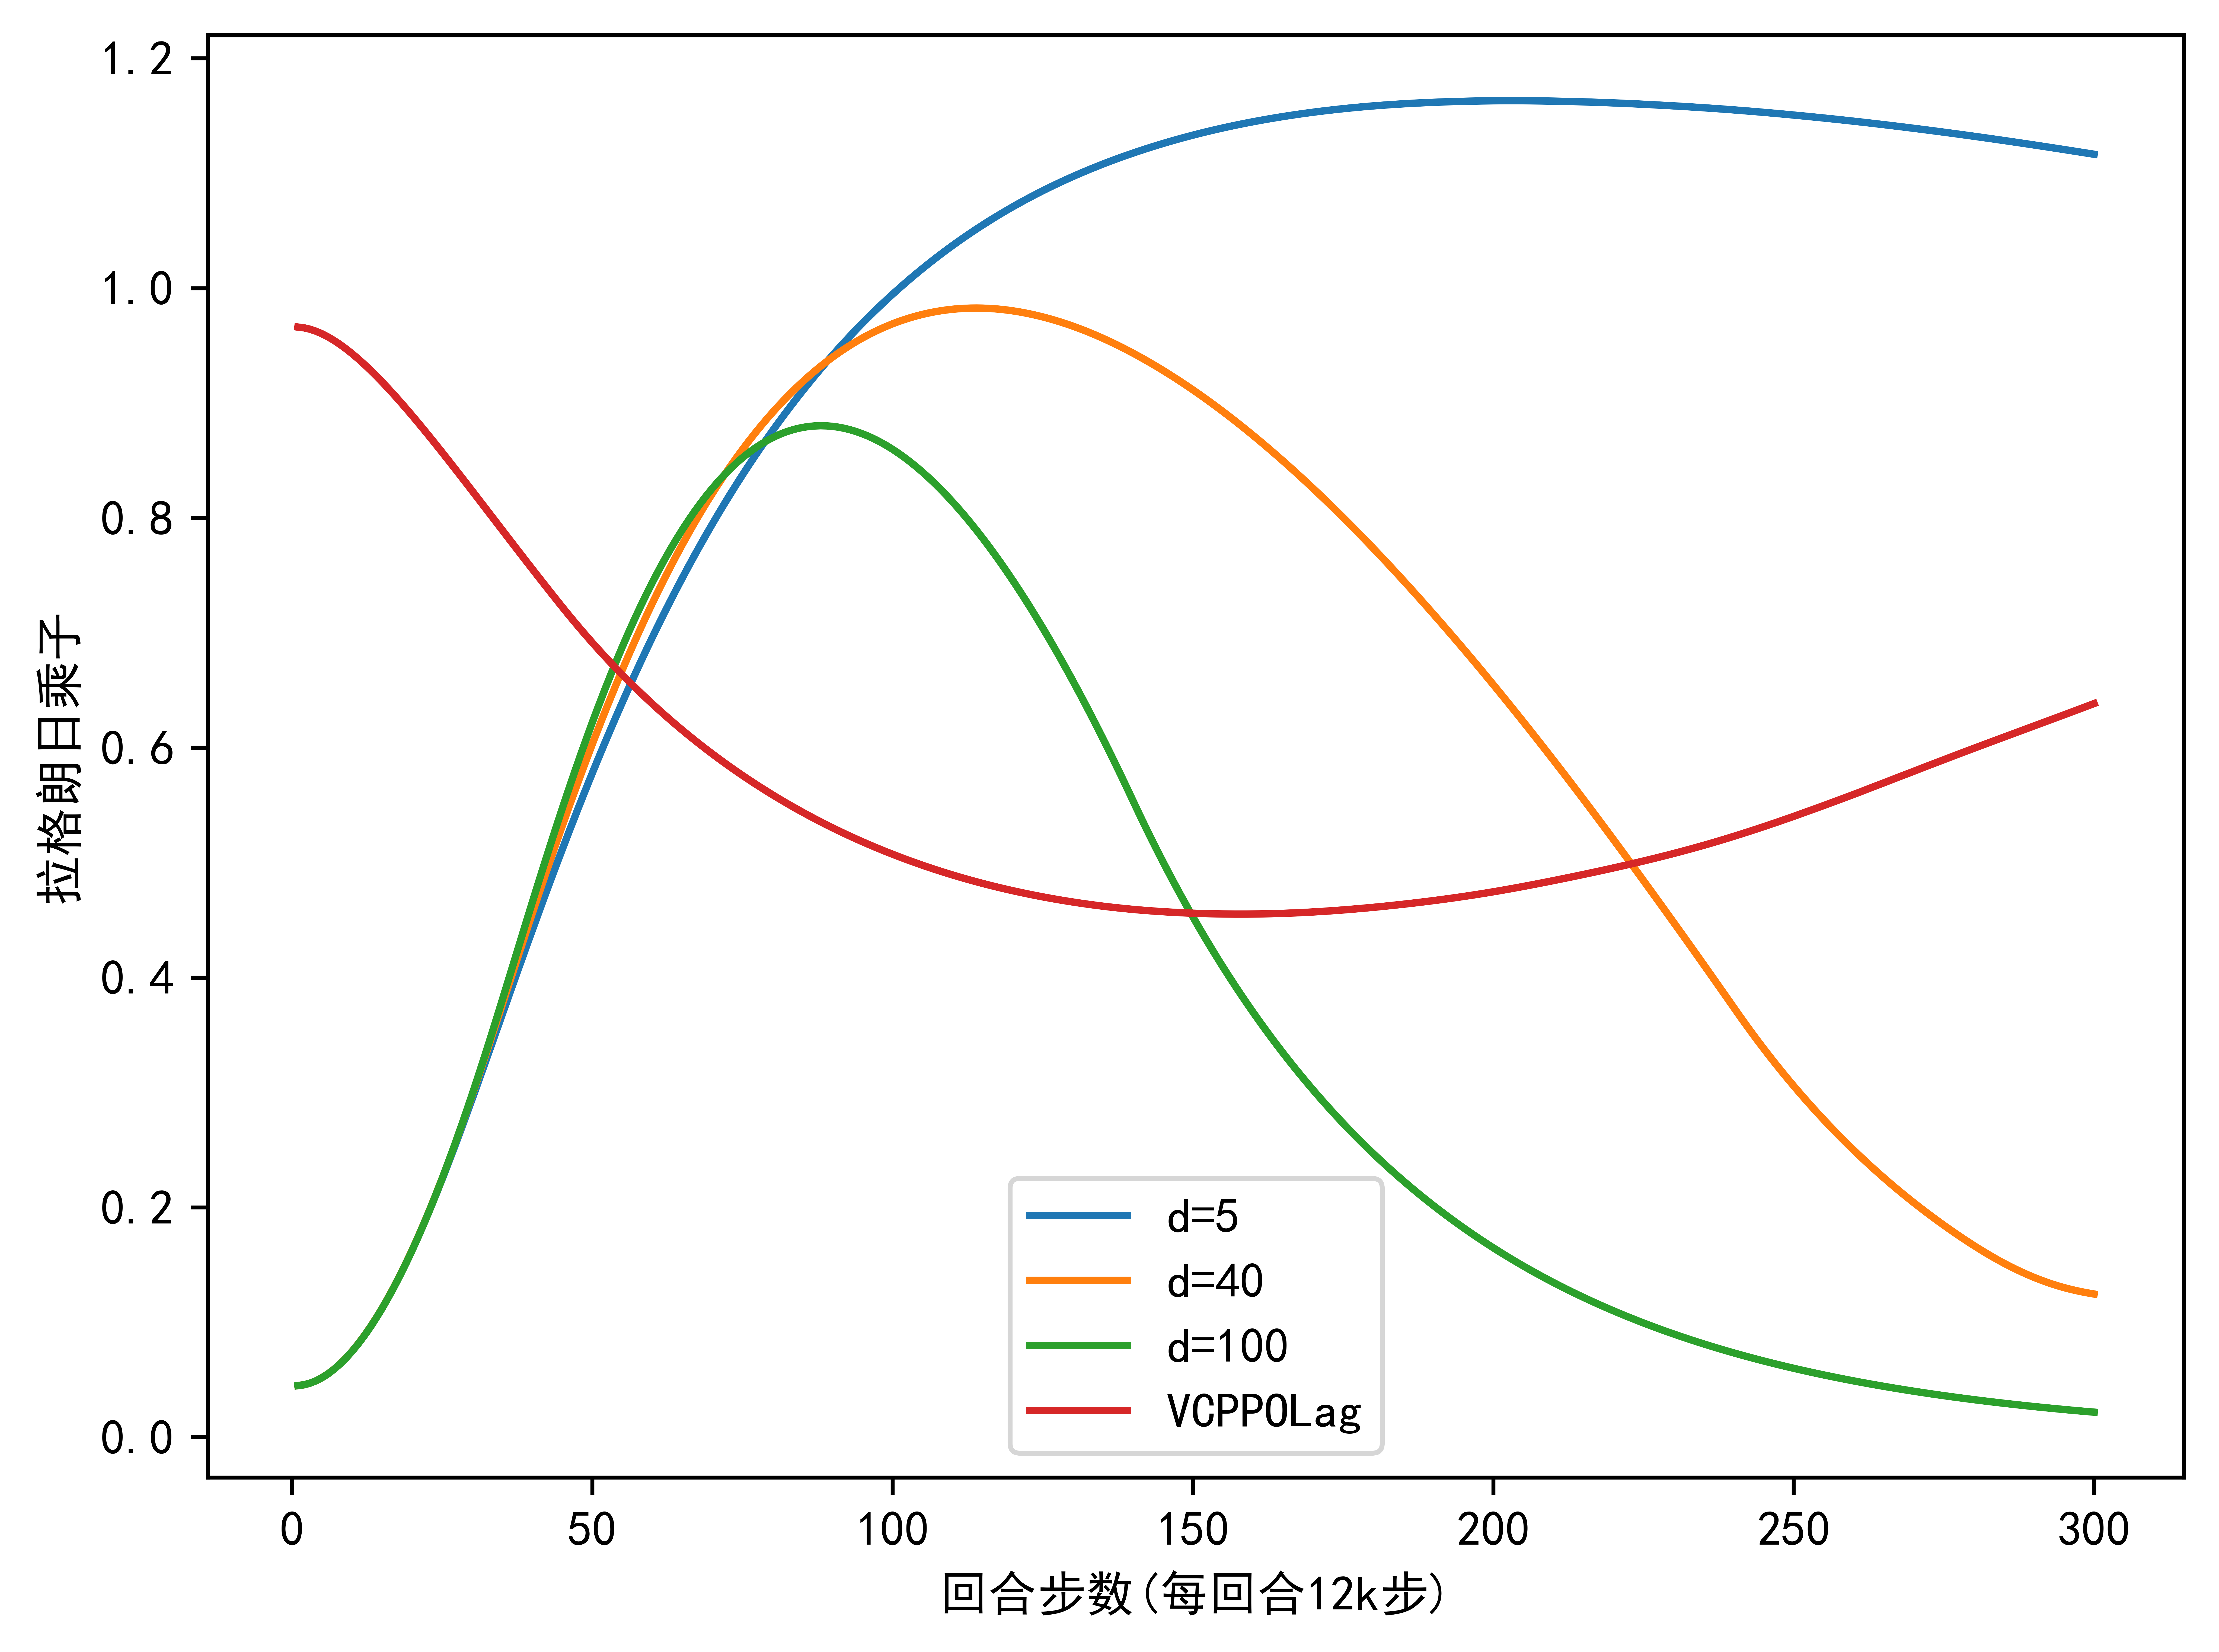
\includegraphics[width=0.9\linewidth]{chapter4/vccmpLag.png}
        \caption{Lag comparison}
        \label{fig:lag}
    \end{subfigure}
    % 添加整体标题和标签
    \caption{VCPPOLag实验结果比较(奖励函数滑动平均0.90)}
    \label{fig:vcppolag}
\end{figure}
实验结果表明,PPOLag算法受制于不恰当的成本阈值设置,展现出了一种先降后升的成本反弹现象。
具体来说,当成本阈值设置为40和100时,观察到随着拉格朗日乘子的调整(如\autoref{fig:lag}所示),
成本呈现出不同程度的上升趋势,进而导致约束满足性的降低。
相反,在成本阈值设为5和40的情况下,智能体的策略在初始阶段变得过分保守,使其在稀疏奖励的环境下难以探索并获得完成过渡任务的终端奖励。

对于PPOLag算法而言,训练初期,由于智能体行为频繁违反垂直速度约束(前100回合),导致成本价值函数网络迅速收敛,使得智能体能够迅速学习到不违反约束的策略。
在此阶段,理应观察到拉格朗日乘子的下降,以辅助智能体探索最优策略,类似于成本阈值设定为100的PPOLag算法。然而,当$d=100$时,尽管智能体探索出了过渡策略,
训练后期却因拉格朗日乘子过小而缺乏足够的约束惩罚,导致约束成本上升。;当$d=40$时,智能体本应进行适量的探索,但由于拉格朗日乘子的更新步长取决于
$d_{i}-J_{C_{i}}(\pi)$控制,乘子下降过缓,削弱了探索效果,使策略趋向于保守解;当$d=5$时,拉格朗日乘子几乎一直处于上升状态。
无法获得有效的探索进行训练。
% 在第三章中,对PPOLag算法在无风条件下的表现进行了探讨。结果表明,该算法在无干扰的确定性环境中能够表现出色,主要因为训练数据不受噪声影响,
% 使得值函数和策略函数训练的方差较低\autoref{fig:loss_cmp}。
% 然而,一旦环境中引入干扰,从监督学习的视角出发,我们发现数据标签会出现波动,这降低了提供给智能体的有效信息量,继而可能导致训练过程的失败。
% \begin{figure}[htbp]
%     \centering
%     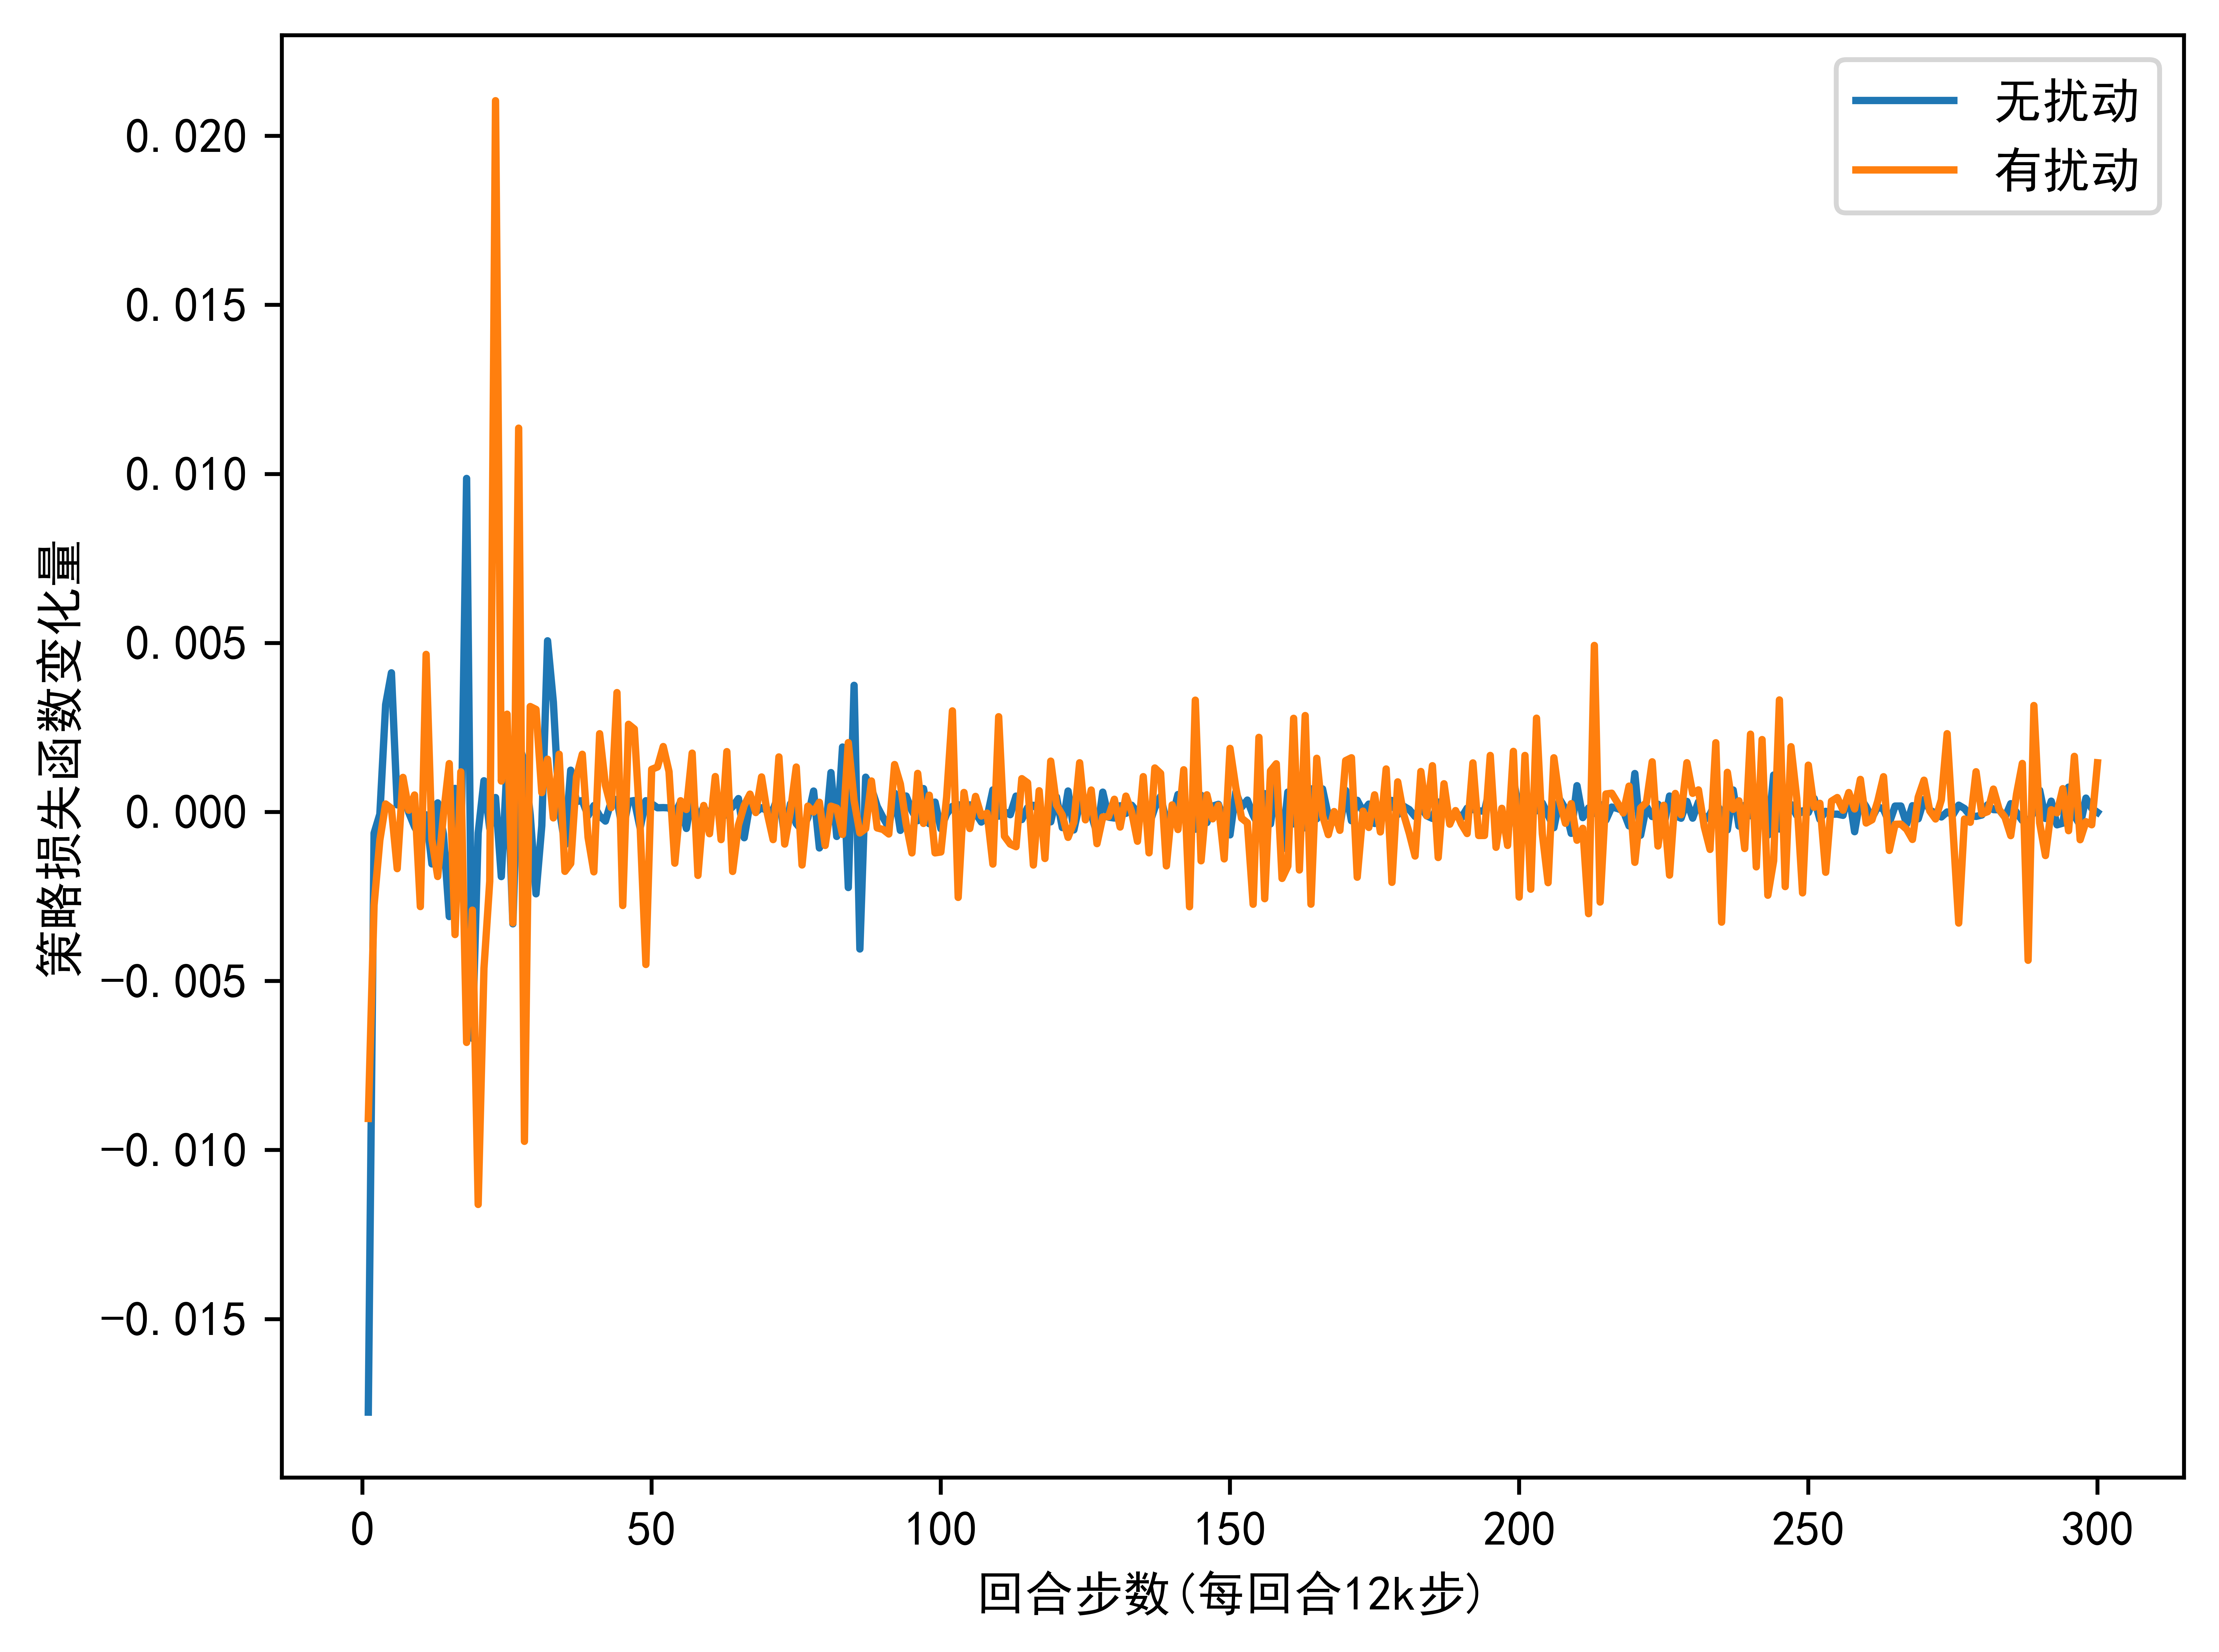
\includegraphics[width=0.75\textwidth]{chapter4/loss.png}
%     \caption{\label{fig:loss_cmp}策略方差对比}
% \end{figure}

而VCPPOLag则令拉格朗日乘子先下降保证不影响到智能体的探索同时学习约束成本价值函数,在探索到过渡策略后再令拉格朗日乘子上升保证不违反约束(150-300回合)。
同时VCPPOLag并不受环境噪声的影响,因为拉格朗日乘子会一直下降直到无人机完成过渡任务。同时可以观察到VCPPOLag算法在训练初期虽然成本函数较高,但伴随着
拉格朗日乘子的上升,智能体可以很快的学会如何满足约束,因为此时约束成本值函数已经接近稳定。在本文这种奖励函数主要由终端奖励构成的设定下,VCPPOLag相比于PPOLag
具备更好的性能,同时对参数的鲁棒性更好,但对于持续性任务,例如,四足机器人奔跑任务中,VCPPOLag的适用性就会变差,因为此时我们需要对每个状态定义一个价值的下届,
这增加了问题的求解难度。

为了更进一步说明VCPPOLag对过渡任务的有效性,我们全部采用300回合内性能最佳的模型以相同的初始状态与环境对算法进行逆过渡飞行实验仿真:
\begin{figure}[H]
    \centering
    % 第一行
    \begin{subfigure}{.5\textwidth}
        \centering
        \includegraphics[width=1.1\linewidth]{chapter4/Vx.png}
        \caption{水平速度}
        \label{fig:vxcmp}
    \end{subfigure}%
    \hfill % 在子图之间添加一些空间
    \begin{subfigure}{.5\textwidth}
        \centering
        \includegraphics[width=1.1\linewidth]{chapter4/Vz.png}
        \caption{垂向速度}
        \label{fig:vzcmp}
    \end{subfigure}
    % 换行,开始第二行
    \\
    % 第二行
    \begin{subfigure}{.5\textwidth}
        \centering
        \includegraphics[width=1.1\linewidth]{chapter4/Theta.png}
        \caption{俯仰角}
        \label{fig:vxcmp}
    \end{subfigure}%
    \hfill % 在子图之间添加一些空间
    \begin{subfigure}{.5\textwidth}
        \centering
        \includegraphics[width=1.1\linewidth]{chapter4/q.png}
        \caption{俯仰角速率}
        \label{fig:vzcmp}
    \end{subfigure}
    % 添加整体标题和标签
    \caption{过渡轨迹对比}
    \label{fig:backtransitioncmp}
\end{figure}

从\autoref{fig:backtransitioncmp}的分析中得知,当成本阈值$d=5$时,智能体已经拥有了可以接受的逆过渡策略,可以达到较低的速度和接近90$\circ$的状态。
然而,智能体未能进一步优化其策略以满足终端约束,这一局限性源自于较高的拉格朗日乘子,该乘子在一定程度上抑制了智能体的进一步探索。
对于$d=40$的情况,观察到智能体的俯仰角和速度持续波动,这表明智能体仍在探索阶段。当$d=100$时,智能体以更高的约束成本完成了过渡任务,
VCPPOLag算法却表现出更低的约束违反次数,成功完成了任务。此结果说明了VCPPOLag在优化约束满足性方面的先进性,相较于将拉格朗日乘子作用在约束成本上,
它能够在保持任务完成的同时,显著减少约束违反的发生。
\subsubsection{鲁棒对抗性能验证}
在本小节中,我们旨在验证算法的鲁棒性能与泛化性能,并首先确立了抗干扰性能的评估标准。无人机的抗干扰性能通过三个主要维度进行评估:确定性环境、训练分布和测试分布。
其中,确定性环境指无扰动条件下的场景,已在第三章进行了详细讨论;训练分布是根据\autoref{tab:paramdisturbance}所定义的环境分布,其代表了智能体的鲁棒性;
测试分布则指超出训练分布范围的环境分布,通常来说它表征了无人机的泛化性能。此项定义基于一个事实:在实际应用中,对环境分布进行精确的先验假设通常是不可行的。
因此,评估算法在面对未曾见过的测试分布下的性能成为抗干扰性能的重要标准,测试分布如\autoref{tab:paramunseendisturbance}。
\begin{table}
    \centering
    \caption{模型测试分布}
    \label{tab:paramunseendisturbance}
    \begin{tabular*}{0.8\textwidth}{@{\extracolsep{\fill}}lll}
        \toprule
        扰动类型 & 噪声分布 & 参数变化范围 \\
        \midrule
        质量扰动\( \left [ kg \right ]  \) & 均匀分布 &  \( [0.8,0.95]\cup[1.05,1.2] \)\\
        转动惯量扰动\( \left [ kg \cdot m^{2} \right ]  \) & 均匀分布 & \(  [0.8,0.95]\cup[1.05,1.2]  \) \\
        升力系数\(C_{L}\) & 均匀分布 & \( [0.6,0.8]\cup[1.2,1.4]  \) \\
        阻力系数\(C_{D}\) & 均匀分布 & \( [0.6,0.8]\cup[1.2,1.4]  \) \\
        俯仰力矩系数\(C_{m} \) & 均匀分布 & \( [0.6,0.8]\cup[1.2,1.4]  \) \\
        传感器信号时滞\( \left [ s \right ]  \) & 指数分布 & \(\lambda\in  \text{Uniform}[ 125,250] \) \\
        俯仰角传感器误差\( \left [ rad \right ]  \) & 高斯分布 & \(\mu = 0.0 ,\sigma =  6.325 \cdot 10^{-3}\) \\
        角速率传感器误差\( \left [ rad/s \right ]  \) & 高斯分布 & \( \mu = 0.0 ,\sigma = 6.325 \cdot 10^{-3}\) \\
        速度传感器误差\( \left [ m/s \right ]  \) & 高斯分布 & \( \mu = 0.0 ,\sigma = 0.029 + 0.2 \) \\
        常值风扰动\( \left [ m/s \right ]  \) & 均匀分布 & \( [-6,-4]\cup[4,6] \)  \\
        阵风扰动开始时间\( \left [ s \right ]\) &均匀分布 & [0,10]\\
        \bottomrule
    \end{tabular*}
\end{table}

结合鲁棒对抗的VCPPOLag与并未结合鲁棒对抗的训练过程示意图如下:
\begin{figure}[htbp]
    \centering
    \includegraphics[width=0.75\textwidth]{chapter4/ra.png}
    \caption{\label{fig:ra}鲁棒对抗训练对比(滑动平均0.94)}
\end{figure}

实验结果表明,伴随着训练回合的增加,对手策略不断优化,鲁棒对抗正逐渐发挥作用,对训练性能产生影响,而在智能体训练初期,
由于对手策略网络尚未学习到如何合理对抗,因此奖励回报会高于无鲁棒对抗。

下面对鲁棒对抗的鲁棒性进行验证,针对\autoref{tab:paramdisturbance}中的干扰,使用不同的种子进行100次蒙特卡洛仿真,成功率为96.67$\%$,其中成功逆过渡飞行状态轨迹如\autoref{fig:transitionstate}:
\begin{figure}[H]
    \centering
    \begin{subfigure}{.55\textwidth}
        \centering
        \includegraphics[width=\linewidth]{chapter4/winddisturbance/x.png}
        \label{fig:sub1-1}
    \end{subfigure}% 
    \begin{subfigure}{.55\textwidth}
        \centering
        \includegraphics[width=\linewidth]{chapter4/winddisturbance/height.png}
        \label{fig:sub2-1}
    \end{subfigure}
    \caption{干扰下逆过渡状态示意图(上)}
    \label{fig:transitionstate-up}
\end{figure}
\begin{figure}[H]
    \centering
    % 第二行
    \begin{subfigure}{.55\textwidth}
        \centering
        \includegraphics[width=\linewidth]{chapter4/winddisturbance/Vx.png}
        \label{fig:sub3-2}
    \end{subfigure}
    \begin{subfigure}{.55\textwidth}
        \centering
        \includegraphics[width=\linewidth]{chapter4/winddisturbance/Vz.png}
        \label{fig:sub4-2}
    \end{subfigure}
    % 第三行
    \begin{subfigure}{.55\textwidth}
        \centering
        \includegraphics[width=\linewidth]{chapter4/winddisturbance/Theta.png}
        \label{fig:sub5-2}
    \end{subfigure}
    \begin{subfigure}{.55\textwidth}
        \centering
        \includegraphics[width=\linewidth]{chapter4/winddisturbance/q.png}
        \label{fig:sub6-2}
    \end{subfigure}
    \caption{干扰下逆过渡状态示意图(下)}
    \label{fig:transitionstate-down}
\end{figure}


如图,可以看出图中展示了在遭受干扰的情况下,智能体能够在较短的时间内,且只需较小的高度调整,就顺
利完成逆过渡任务。

下面对鲁棒对抗下的泛化性能进行验证,针对\autoref{tab:paramunseendisturbance}中未见过的干扰,使用不同的种子进行30次蒙特卡洛仿真,
成功率为63$\%$,失败的无人机飞行状态如\autoref{fig:failed}所示:
\begin{figure}[H]
    \centering
    % 第一行
    \begin{subfigure}{.55\textwidth}
        \centering
        \includegraphics[width=\linewidth]{chapter4/winddisturbance/windfailed/Vx.png}
        \label{fig:sub1}
        \end{subfigure}% <-- 注意这里的百分号
        \begin{subfigure}{.55\textwidth}
        \centering
        \includegraphics[width=\linewidth]{chapter4/winddisturbance/windfailed/Vz.png}
        \label{fig:sub2}
        \end{subfigure}
    % 第二行
    \begin{subfigure}{.55\textwidth}
        \centering
        \includegraphics[width=\linewidth]{chapter4/winddisturbance/windfailed/Theta.png}
        \label{fig:sub3}
    \end{subfigure}% <-- 注意这里的百分号
    \begin{subfigure}{.55\textwidth}
        \centering
        \includegraphics[width=\linewidth]{chapter4/winddisturbance/windfailed/q.png}
        \label{fig:sub4}
    \end{subfigure}
\caption{逆过渡失败飞行状态}
\label{fig:failed}
\end{figure}
如图可以看出,无人机在面对未见过的测试分布时,过渡性能表现不佳,其过渡终端角度误差过大。
其主要原因是悬停状态在训练数据中占据比重较低,导致无人机在悬停状态下的抗干扰能力较差,在实际应用中,
可以考虑扩大悬停控制器的容许控制范围进行补偿。

鲁棒对抗下与无鲁棒对抗下的过渡性能表现如\autoref{tab:ra}和\autoref{tab:nora}所示,在面对测试分布时,
无鲁棒对抗的智能体性能大幅度下降,尤其是终端角度误差,在失败时最大可接近$20^{\circ}$的误差,而对于鲁棒对抗下的智能体,
虽然其过渡成功率仅有53.3\%,但其过渡失败下的性能表现处于可接受状态,误差最大为$10^{\circ}$
\begin{table}[h]
    \centering
    \caption{鲁棒对抗性能验证}
    \label{tab:ra}
    \small % 减小字体大小
    \begin{tabular*}{0.85\textwidth}{@{\extracolsep{\fill}}lccccccc}
        \toprule
        性能表现(均值/方差) & 确定环境 & 训练分布 & 测试分布 \\
        \midrule
        成功率 & 100\% & 96.67\% & 53.3\% \\
        奖励回报 & \(121.1\pm1.6\) & \(110.6\pm18.1\) & \(71.13\pm56.75\) \\
        约束成本 & \(6.8\pm11.0\) & \(2.0\pm2.25\) & \(35.93\pm59.17\) \\
        平均过渡时间 & \(3.5\pm0.2\) & \(2.93\pm1.44\) & \(5.54\pm4.16\) \\
        平均高度最大变化 & \(0.48\pm0.22\) & \(0.09\pm0.07\) & \(1.17\pm4.99\) \\
        终端角度误差(成功/失败) & \(1.0\pm0.2 \setminus - \) & \(1.19\pm2.3 \setminus 5.7\pm0 \) & \(4.87\pm1.14 \setminus 8.67\pm 0.18\) \\
        终端速度误差(成功/失败) & \(0.31\pm0.01 \setminus - \) & \(0.38\pm0.14 \setminus 0.6\pm0 \) & \(0.34\pm0.09 \setminus 0.85\pm0.60 \) \\
        \bottomrule
    \end{tabular*}
\end{table}

\begin{table}[h]
    \centering
    \caption{无对抗性能验证}
    \label{tab:nora}
    \small % 减小字体大小
    \begin{tabular*}{0.85\textwidth}{@{\extracolsep{\fill}}lccccccc}
        \toprule
        性能表现(均值/方差) & 确定环境 & 训练分布 & 测试分布 \\
        \midrule
        成功率 & 100\% & 100\% & 30.0\% \\
        奖励回报 & \(125.2\pm1.27\) & \(123.4\pm10.6\) & \(47.1\pm49.9\) \\
        约束成本 & \(4.4\pm6.65\) & \(0.5\pm1.52\) & \(50.2\pm54.2\) \\
        平均过渡时间 & \(2.52\pm0.01\) & \(2.7\pm0.48\) & \(7.7\pm3.6\) \\
        平均高度最大变化 & \(0.09\pm0.07\) & \(0.30\pm0.23\) & \(1.6\pm1.1\) \\
        终端角度误差(成功/失败) & \(3.7\pm0.11 \setminus - \) & \(0.5\pm1.1 \setminus - \) & \(1.8\pm1.7 \setminus 5.7\pm 20.6\) \\
        终端速度误差(成功/失败) & \(0.4\pm0.01 \setminus - \) & \(0.4\pm0.1 \setminus - \) & \(0.5\pm0.1 \setminus 0.9\pm3.6 \) \\
        \bottomrule
    \end{tabular*}
\end{table}

综上所示,鲁棒对抗能以确定环境和训练分布下逆过渡飞行性能表现的微小下降获得较好的测试分布下的泛化性能表现。在‘对手’风扰的攻击下,即使无人机并未达到指定的终端状态误差范围,但其仍然具备
接近终端状态的能力,而仅适用领域随机化进行训练的无人机在面对测试分布时性能表现较差,其终端角度误差与终端速度误差方差较大,不利于真实世界的迁移。

\section{考虑执行器约束的策略改进}
在上述快速定高逆过渡实验中,强化学习算法虽然表现出较短的过渡时间与较低的高度变化,却也存在潜在的安全威胁,例如:在逆过渡任务的开始阶段,强化学习算法
要求控制量快速上升达到峰值,然而由于真实世界执行器存在速率限制,这不仅在难以实现,同时还会给执行器带来损伤。
针对上述问题,要求在优化无人机快速定高过渡时,不仅应该关注其过渡过程中的性能表现,还应考虑对控制量进行优化,保证真实世界的可执行,因此,本节将针对执行器约束,提出相应的强化学习解决方案,并对无人机进行仿真性能验证,
更进一步完善无人机快速定高转换过渡策略。
\subsection{考虑执行器约束的快速定高转换逆过渡问题建模}
根据\autoref{eq:dynamics}以及无人机纵向模型进行水平飞行状态以及悬停状态的工作特点进行控制量配平,结果如\autoref{fig:trim}
\begin{figure}[htbp]
    \centering
    \begin{minipage}{0.5\linewidth}
        \centering
        \includegraphics[width=\linewidth]{chapteren/trimspeed.png} % 宽度调整为minipage的100%
        \caption{螺旋桨转速归一化}
        \label{fig:reward_cmp3}
    \end{minipage}%
    \hfill % 选择性地填充两个minipage之间的空间,也可以省略以紧挨着放置
    \begin{minipage}{0.5\linewidth}
        \centering
        \includegraphics[width=\linewidth]{chapteren/trimele.png} % 宽度调整为minipage的100%
        \caption{舵机偏转归一化}
        \label{fig:cost_cmp3}
    \end{minipage}
    \caption{配平控制量示意图}
    \label{fig:trim}
\end{figure}


可以发现,过渡过程的初始控制量距离水平飞行的配平控制量差异较大,特别是舵机偏转角度要求从0$\circ$瞬间变换至$90\circ$,这在实践中几乎无法满足。
产生这一现象的原因正是因为对于时间最优的性能指标,控制量具备‘Bang-Bang’的控制量特点,总是在最大值与最小值之间进行切换,如\autoref{fig:gpops}中
的GPOPS-II控制量。而对于强化学习而言,固定的终端高奖励结合折扣因子也同样会将奖励最大化问题近似成时间最小化问题,即:
\begin{align}
    \min  \underset{\tau \sim \pi }{\mathrm{E}}\left[\sum_{t=0}^{\infty} \gamma^{t}\kappa\right]=\min t_{f}
\end{align}
为了解决上述问题,我们必须重新形式化无人机逆过渡任务中的性能指标,考虑控制量的变化,以保证无人机在完成逆过渡任务的同时具有可以容许的控制量变化。
因此,考虑最小化控制器速率,其性能指标定义为:
\begin{align}
    J & = \int_{t_{0}}^{t_{f}}\left[1+\alpha (\left |\dot \delta_{y} \right |+\left |\dot \omega_{p} \right |)\right] d t
\end{align}
其中,$\alpha$作为超参数,控制着时间和执行器控制速率的权衡。

由于强化学习和最优控制通常考虑从初始状态开始进行优化,因此控制速率约束通常限制的是初始时刻控制量的右导数而忽略了左导数,所以上述性能指标仍无法解决逆过渡初始控制量与配平状态控制量的误差。
为此,考虑如下初始控制量约束:
\begin{align}
    \omega_{p}(t_{0}) = \omega_{p,trim} \\
    \delta_{y}(t_{0}) = \delta_{y,trim}
\end{align}

综上,考虑执行器约束的涵道无人机快速定高过渡问题的定义如下:

涵道无人机满足如\autoref{eq:dynamics}所示的运动学与动力学方程,初始飞行状态如由初始俯仰角根据水平模态力学特性配平求得,在过渡过渡中满足
\autoref{eq:constraints1}中的角速度和控制量约束,以及\autoref{eq:constraints2}中的垂向速度约束,并过渡至如\autoref{eq:initial_final_state}所示的指定末端状态,
且使\autoref{eq:optimization}代价函数最小。
\begin{align}
    \label{eq:optimization}
    J = \int_{t_{0}}^{t_{f}}\left [ 1+\alpha (\left|\dot{u}\right| ) \right ]dt +\Phi (u(t_{0}))\\
\textbf{其中,} \Phi (u(t_{0}))=\left \| u(t_{0})-u_{trim} \right \|_{2}^{2} 
\end{align}
式中,$\alpha$与为超参数。

综上所述,我们重新定义了考虑执行器速率约束的无人机逆过渡问题。
\subsection{利普希茨网络与动作正则化}
常见的强化学习算法在处理执行器速率问题时,通常采取将上一时刻的动作增广到状态空间中,并在奖励函数中对前后动作的二范数进行惩罚\cite{kaufmann2023champion}。
然而,实际上这种惩罚的大小在真实中往往难以确定,过小的惩罚会令智能体忽略动作的影响,过大的惩罚有可能会导致探索受限。
为此,我们结合\parencite{song2023lipsnet}中提出的利普希茨网络并结合动作正则化技术对执行器速率约束问题进行改进,利普希茨网络的结构如\autoref{fig:lips}所示。
\begin{figure}[htbp]
    \centering
    \includegraphics[width=0.75\textwidth]{chapteren/lipts.png}
    \caption{\label{fig:lips}利普希茨网络结构}
\end{figure}

利普希茨网络的输出具有以下特点:
\begin{align}
    \label{eq:lipsproof}
    \left\|\nabla_{x} f(x)\right\|=K \cdot\left\|\nabla \frac{f}{\|\nabla f\|+\epsilon}\right\| \\
    =K \cdot\left\|\frac{\nabla f(\|\nabla f\|+\epsilon)-f(\nabla(\|\nabla f\|+\epsilon))^{\top}}{(\|\nabla f\|+\epsilon)^{2}}\right\|=K \cdot\left\|\frac{\nabla f}{\|\nabla f\|+\epsilon}\right\| \leq K
\end{align}
由\autoref{eq:lipsproof}可以发现,利普希茨网络可以保证网络具备局部利普希茨连续的特点,并保证其局部利普希茨常数不超过$K$,其中$K$由网络学习并通过softplus激活函数控制保证不超过1。
因此,利普希茨网络可以通过控制网络的利普希茨常数(Lipschitz constant),从而保证网络输出对于输入的微小变化不会有过大的波动。

在实际实验中,利普希茨网络同样会面临探索与利用的困境。因为初始利普希茨常数往往很难确定,同时,由于该网络仅能保证网络具有小于$K$的局部利普希茨连续性。
因此为了更好地对动作加以限制,我们采用了前后状态的策略分布JS散度和初始状态下的策略输出的均方误差对动作进行正则化。

首先,执行器速率约束问题可以定义为以下优化问题:
\begin{align}
    \arg \min _{\pi_{\theta}}&\mathcal{D}_{\mathrm{J}}\left(\pi_{\theta}(\cdot \mid s_{t}) \| \pi_{\theta}(\cdot \mid s_{t+1})\right)\\
\end{align}
其中,$\pi_{\theta}(\cdot \mid s_{t})$表示智能体在状态$s_{t}$下的高斯动作分布,因此我们可以借助Jeffreys散度来
衡量智能体在当前状态动作分布与其后续状态的动作分布之间的差异,Jeffreys散度由于能够克服KL散度的非对称性缺陷而被选用,其定义为:其定义为:$J(P|Q) = KL(P|Q)+KL(Q|P)$。

所以我们可以对策略网络进行如下更新:
\begin{align}
    \theta &\leftarrow \theta-\eta \nabla L^{Action}(\theta)\\
    L^{Action}(\theta)&={D}_{\mathrm{JS}}\left(\pi_{\theta}(\cdot \mid s_{t}) \| \pi_{\theta}(\cdot \mid s_{t+1})\right)+MSE(u_{\theta}(s_{0})-u_{trim})
\end{align}
其中,Jeffreys散度由于能够克服KL散度的非对称性缺陷而被选用,其定义为:其定义为:$J(P|Q) = KL(P|Q)+KL(Q|P)$,初始状态下的策略输出由于是一个分布无法对其求出梯度,因此采用重采样方法使其可以进行梯度运算
\subsection{实验仿真与验证}
在本小节中,我们将针对利普希茨网络结合动作正则化进行了有无干扰下的实验对比。为了更好地说明动作光滑,我们使用了平均动作变化率来进行动作光滑的评估:
\begin{align}
    \xi(\pi)  = \mathbb{E}_{\tau \sim \rho_{\pi}}\left[\frac{1}{T} \sum_{t = 1}^{T}\left\|a_{t}-a_{t-1}\right\|\right]
    \end{align}
无干扰下,结合动作正则化的利普希茨后的逆过渡飞行实验如下:
\begin{figure}[H]
    \centering
    \begin{subfigure}{.46\textwidth}
        \centering
        \includegraphics[width=\linewidth]{chapteren/X.png}
        \caption{横向位移}
        \label{fig:actionsub1}
    \end{subfigure}% <-- 注意这里的百分号
    \begin{subfigure}{.46\textwidth}
        \centering
        \includegraphics[width=\linewidth]{chapteren/Z.png}
        \caption{垂直位移}
        \label{fig:actionsub2}
    \end{subfigure}
    \begin{subfigure}{.46\textwidth}
        \centering
        \includegraphics[width=\linewidth]{chapteren/Vx.png}
        \caption{横向速度}
        \label{fig:actionsub3}
    \end{subfigure}% <-- 注意这里的百分号
    \begin{subfigure}{.46\textwidth}
        \centering
        \includegraphics[width=\linewidth]{chapteren/Vz.png}
        \caption{垂直速度}
        \label{fig:actionsub4}
    \end{subfigure}
    \begin{subfigure}{.46\textwidth}
        \centering
        \includegraphics[width=\linewidth]{chapteren/Theta.png}
        \caption{俯仰角}
        \label{fig:actionsub5}
    \end{subfigure}% <-- 注意这里的百分号
    \begin{subfigure}{.46\textwidth}
        \centering
        \includegraphics[width=\linewidth]{chapteren/q.png}
        \caption{俯仰角速率}
        \label{fig:actionsub6}
    \end{subfigure}
    \begin{subfigure}{.46\textwidth}
        \centering
        \includegraphics[width=\linewidth]{chapteren/ele.png}
        \caption{升降舵偏转}
        \label{fig:actionsub7}
    \end{subfigure}% <-- 注意这里的百分号
    \begin{subfigure}{.46\textwidth}
        \centering
        \includegraphics[width=\linewidth]{chapteren/speed.png}
        \caption{螺旋桨转速}
        \label{fig:actionsub8}
    \end{subfigure}
    \caption{动作优化对比示意图}
    \label{fig:action_smooth}
\end{figure}
我们可以看出,动作正则化和利普希茨网络以过渡时间为代价成功地令原本Bang-Bang的控制量曲线光滑。
其中,
\begin{table}[h]
    \centering
    \caption{平均动作变化率}
    \label{tab:nora}
    \small % 减小字体大小
    \begin{tabular*}{0.85\textwidth}{@{\extracolsep{\fill}}lccccccc}
        \toprule
        平均动作变化率 & 螺旋桨转速 & 舵机偏转 \\
        \midrule
        Lips+JS & 0.3546 & 0.3786\\
        Vanilla & 1.1318 & 2.2807 \\
        \bottomrule
    \end{tabular*}
\end{table}

下面对考虑干扰下的利普希茨网络结合动作正则化进行验证,选用训练分布\autoref{tab:paramdisturbance},进行30次逆过渡飞行仿真验证:
\begin{figure}[H]
    \centering
    \begin{subfigure}{.46\textwidth}
        \centering
        \includegraphics[width=\linewidth]{chapteren/action/Vx.png}
        \caption{水平速度}
        \label{fig:sub1}
    \end{subfigure}% <-- 注意这里的百分号
    \begin{subfigure}{.46\textwidth}
        \centering
        \includegraphics[width=\linewidth]{chapteren/action/Vz.png}
        \caption{垂向速度}
        \label{fig:sub2}
    \end{subfigure}
    \begin{subfigure}{.46\textwidth}
        \centering
        \includegraphics[width=\linewidth]{chapteren/action/Theta.png}
        \caption{横俯仰角}
        \label{fig:sub3}
    \end{subfigure}% <-- 注意这里的百分号
    \begin{subfigure}{.46\textwidth}
        \centering
        \includegraphics[width=\linewidth]{chapteren/action/q.png}
        \caption{俯仰角速率}
        \label{fig:sub4}
    \end{subfigure}
    \begin{subfigure}{.46\textwidth}
        \centering
        \includegraphics[width=\linewidth]{chapteren/action/speed.png}
        \caption{螺旋桨转速}
        \label{fig:sub5}
    \end{subfigure}% <-- 注意这里的百分号
    \begin{subfigure}{.46\textwidth}
        \centering
        \includegraphics[width=\linewidth]{chapteren/action/ele.png}
        \caption{舵机偏转}
        \label{fig:sub6}
    \end{subfigure}
    \caption{动作优化飞行示意图}
    \label{fig:action_smooth1}
\end{figure}
由\autoref{fig:action_smooth1}可以看出,结合动作正则化的利普希茨网络并不会影响到策略网络的抗干扰能力,并且
可以在牺牲过渡时间和约束违反次数的条件下,降低平均动作变化率,验证了利普希茨网络结合动作化方法的有效性。
\section{本章总结}
在本章中,我们考虑了现实世界中不可避免的不确定性干扰与执行器速率约束,并对第三章提出的算法进行了精细化改进。
首先我们建立了环境中可能的潜在干扰分布,并针对PPOLag算法在干扰下难以确定成本阈值的缺陷,提出了一种基于值函数约束的改进方法,
并验证了基于值函数约束方法的有效性,其次,我们结合鲁棒对抗框架对逆过渡方法进行改进,表明了鲁棒对抗可以优化无人机在未知分布下的
逆过渡性能表现,最后我们使用利普希茨网络结合动作正则化技术,对无人机在逆过渡过程中的平均动作变化率进行优化,说明了结合正则化的利普希茨网络
能够在不降低系统鲁棒性的同时有效解决无人机逆过渡飞行中的控制量’Bang-Bang‘问题。

\chapter{总结与展望}
\section{工作总结}
涵道风扇尾座式无人机是一种正在发展的新型固定翼垂直起降飞行器,其介于垂直悬停和水平飞行状态之间的过渡过程动力学特性复杂,
控制难度大。传统过渡控制方法往往选择牺牲过渡性能从而保证过渡控制的稳定性,而基于轨迹优化的方法往往因其运算量使得难以在
嵌入式上在线运行只能离线优化,因此本文聚焦于最小化过渡时间和高度变化的‘快速定高逆过渡’问题,
提出了一种轨迹优化与过渡控制相结合的强化学习控制方案,保证了实时性并提升了过渡性能,本文的主要工作如下:

(1) 本研究构建了涵道风扇式尾座垂直起降无人机的数学模型,这一模型适用于过渡阶段高攻角飞行模态的分析。在探讨无人机
过渡阶段的时间和高度变化这两个关键性能指标时,我们将垂直速度作为一个约束条件,以最小化过渡时间为目标,提出了一种‘快速定高过渡’方式,
给出了其数学问题描述,并在此基础上建立了一个用于强化学习的仿真环境。

(2)针对‘快速定高过渡’的问题,本文将无人机的横向和纵向动作解耦,并以无人机的纵向运动模型为基础,提出了一个结合课程学习的PPOLag训练
方案。通过这一训练方案优化得到的过渡轨迹,在性能上可以与采用伪谱法的GPOPS-II优化轨迹相媲美。通过与总能量控制系统进行对比实验,进一
步验证了我们方案在过渡轨迹优化方面的优势。此外,与传统强化学习算法相比,引入约束的重要性得到了强调。最后,结合横向和纵向的仿真实验,
我们验证了在过渡问题中解耦的可行性。

(3)针对无人机逆过渡过程中外部风干扰和内部模型参数失配的挑战,本文采用了领域随机化技术进行模型训练。面对不确定性环境中常规约束强化学习
算法难以设定准确成本阈值的问题,我们提出了一种基于价值受限的PPOLag(VCPPOLag)算法。该算法通过实验与传统PPOLag算法进行了比较,突显
了在初始状态价值函数上施加约束的重要性。此外,通过蒙特卡洛仿真的方法,我们证实了该策略对抗干扰的有效性,表明了其在处理无人机逆过渡过程
中的风干扰和模型不匹配情况下的鲁棒性。
    
    \section{未来展望}
    
    本文通过强化学习算法对尾座式垂直起降无人机的逆过渡问题进行了深入探究,展现了强化学习在无人机过渡控制乃至整体飞行控制领域的应用潜力。为了在这一领域取得更多突破,作者提出以下研究展望,以期开拓未来的研究路径:
    
    (1) 元学习:考虑到现实世界条件下的复杂性,当前的研究尽管涉及了特定分布下的模型扰动与环境干扰,但对未知环境的适应性仍有限。未来研究可以采用元学习策略,在仿真环境中培养出能快速适应真实世界变化的算法,
    通过在真实世界中收集少量数据进行微调,从而提高策略的泛化能力和应变速度。
    
    (2) 多任务学习研究:本文专注于逆过渡飞行阶段,然而不同的飞行模式背后共享相同的动力学法则。在未来的工作中,计划将悬停、水平飞行等其他飞行模式纳入辅助任务,通过多任务学习框架来促进过渡飞行任务的快速
    学习。此举旨在探索如何设计一个能够应对包括正过渡、悬停、水平飞行在内的多样化任务的综合飞行控制器。
    
    (3) 过渡策略多样性研究:真实世界任务的多样性要求过渡策略的多样化。例如,无人机着陆过程中的逐渐下降策略虽具有相当的控制难度但却十分高效,
    而在正过渡过程中,面对强风干扰,采用侧向飞行可能会减少阻力并提升效率。因此,未来研究中如何巧妙设计奖励函数来诱导无人机在不同环境条件下
    发现最优过渡方法,将是一个研究重点,同时也具有重要的应用价值。



